\documentclass[ALICE,manyauthors]{cernphprep}
%DIF LATEXDIFF DIFFERENCE FILE
%DIF DEL ../version03/main.tex   Fri Oct  4 00:41:11 2019
%DIF ADD main.tex                Fri Oct  4 00:46:29 2019
\usepackage[comma,square,numbers,sort&compress]{natbib}
\usepackage{hyperref}
\usepackage{lineno}
\usepackage{xspace}

\usepackage[T1]{fontenc} % if needed
\usepackage{setspace}
\usepackage{capt-of}
\usepackage{epstopdf}
\usepackage{color}
\usepackage{multirow}
\usepackage{tabu}
 \usepackage[draft]{todonotes}
 \usepackage{float}

\usepackage{tabularx}
\usepackage{changepage}     
\usepackage[figuresright]{rotating}
\usepackage{graphicx} 

%\usepackage{pstricks}
%\usepackage{pst-tree}
%\usepackage[crop=off, runs=2]{auto-pst-pdf}
%\usepackage{pst-pdf}
%\usepackage{ifplatform}
%\usepackage{psfrag}

\newcolumntype{?}{!{\vrule width 2pt}}
\newcolumntype{@}{!{\vrule width 1.5pt}}


\linenumbers
%DIF PREAMBLE EXTENSION ADDED BY LATEXDIFF
%DIF UNDERLINE PREAMBLE %DIF PREAMBLE
\RequirePackage[normalem]{ulem} %DIF PREAMBLE
\RequirePackage{color}\definecolor{RED}{rgb}{1,0,0}\definecolor{BLUE}{rgb}{0,0,1} %DIF PREAMBLE
\providecommand{\DIFaddtex}[1]{{\protect\color{blue}\uwave{#1}}} %DIF PREAMBLE
\providecommand{\DIFdeltex}[1]{{\protect\color{red}\sout{#1}}}                      %DIF PREAMBLE
%DIF SAFE PREAMBLE %DIF PREAMBLE
\providecommand{\DIFaddbegin}{} %DIF PREAMBLE
\providecommand{\DIFaddend}{} %DIF PREAMBLE
\providecommand{\DIFdelbegin}{} %DIF PREAMBLE
\providecommand{\DIFdelend}{} %DIF PREAMBLE
%DIF FLOATSAFE PREAMBLE %DIF PREAMBLE
\providecommand{\DIFaddFL}[1]{\DIFadd{#1}} %DIF PREAMBLE
\providecommand{\DIFdelFL}[1]{\DIFdel{#1}} %DIF PREAMBLE
\providecommand{\DIFaddbeginFL}{} %DIF PREAMBLE
\providecommand{\DIFaddendFL}{} %DIF PREAMBLE
\providecommand{\DIFdelbeginFL}{} %DIF PREAMBLE
\providecommand{\DIFdelendFL}{} %DIF PREAMBLE
%DIF HYPERREF PREAMBLE %DIF PREAMBLE
\providecommand{\DIFadd}[1]{\texorpdfstring{\DIFaddtex{#1}}{#1}} %DIF PREAMBLE
\providecommand{\DIFdel}[1]{\texorpdfstring{\DIFdeltex{#1}}{}} %DIF PREAMBLE
\newcommand{\DIFscaledelfig}{0.5}
%DIF HIGHLIGHTGRAPHICS PREAMBLE %DIF PREAMBLE
\RequirePackage{settobox} %DIF PREAMBLE
\RequirePackage{letltxmacro} %DIF PREAMBLE
\newsavebox{\DIFdelgraphicsbox} %DIF PREAMBLE
\newlength{\DIFdelgraphicswidth} %DIF PREAMBLE
\newlength{\DIFdelgraphicsheight} %DIF PREAMBLE
% store original definition of \includegraphics %DIF PREAMBLE
\LetLtxMacro{\DIFOincludegraphics}{\includegraphics} %DIF PREAMBLE
\newcommand{\DIFaddincludegraphics}[2][]{{\color{blue}\fbox{\DIFOincludegraphics[#1]{#2}}}} %DIF PREAMBLE
\newcommand{\DIFdelincludegraphics}[2][]{% %DIF PREAMBLE
\sbox{\DIFdelgraphicsbox}{\DIFOincludegraphics[#1]{#2}}% %DIF PREAMBLE
\settoboxwidth{\DIFdelgraphicswidth}{\DIFdelgraphicsbox} %DIF PREAMBLE
\settoboxtotalheight{\DIFdelgraphicsheight}{\DIFdelgraphicsbox} %DIF PREAMBLE
\scalebox{\DIFscaledelfig}{% %DIF PREAMBLE
\parbox[b]{\DIFdelgraphicswidth}{\usebox{\DIFdelgraphicsbox}\\[-\baselineskip] \rule{\DIFdelgraphicswidth}{0em}}\llap{\resizebox{\DIFdelgraphicswidth}{\DIFdelgraphicsheight}{% %DIF PREAMBLE
\setlength{\unitlength}{\DIFdelgraphicswidth}% %DIF PREAMBLE
\begin{picture}(1,1)% %DIF PREAMBLE
\thicklines\linethickness{2pt} %DIF PREAMBLE
{\color[rgb]{1,0,0}\put(0,0){\framebox(1,1){}}}% %DIF PREAMBLE
{\color[rgb]{1,0,0}\put(0,0){\line( 1,1){1}}}% %DIF PREAMBLE
{\color[rgb]{1,0,0}\put(0,1){\line(1,-1){1}}}% %DIF PREAMBLE
\end{picture}% %DIF PREAMBLE
}\hspace*{3pt}}} %DIF PREAMBLE
} %DIF PREAMBLE
\LetLtxMacro{\DIFOaddbegin}{\DIFaddbegin} %DIF PREAMBLE
\LetLtxMacro{\DIFOaddend}{\DIFaddend} %DIF PREAMBLE
\LetLtxMacro{\DIFOdelbegin}{\DIFdelbegin} %DIF PREAMBLE
\LetLtxMacro{\DIFOdelend}{\DIFdelend} %DIF PREAMBLE
\DeclareRobustCommand{\DIFaddbegin}{\DIFOaddbegin \let\includegraphics\DIFaddincludegraphics} %DIF PREAMBLE
\DeclareRobustCommand{\DIFaddend}{\DIFOaddend \let\includegraphics\DIFOincludegraphics} %DIF PREAMBLE
\DeclareRobustCommand{\DIFdelbegin}{\DIFOdelbegin \let\includegraphics\DIFdelincludegraphics} %DIF PREAMBLE
\DeclareRobustCommand{\DIFdelend}{\DIFOaddend \let\includegraphics\DIFOincludegraphics} %DIF PREAMBLE
\LetLtxMacro{\DIFOaddbeginFL}{\DIFaddbeginFL} %DIF PREAMBLE
\LetLtxMacro{\DIFOaddendFL}{\DIFaddendFL} %DIF PREAMBLE
\LetLtxMacro{\DIFOdelbeginFL}{\DIFdelbeginFL} %DIF PREAMBLE
\LetLtxMacro{\DIFOdelendFL}{\DIFdelendFL} %DIF PREAMBLE
\DeclareRobustCommand{\DIFaddbeginFL}{\DIFOaddbeginFL \let\includegraphics\DIFaddincludegraphics} %DIF PREAMBLE
\DeclareRobustCommand{\DIFaddendFL}{\DIFOaddendFL \let\includegraphics\DIFOincludegraphics} %DIF PREAMBLE
\DeclareRobustCommand{\DIFdelbeginFL}{\DIFOdelbeginFL \let\includegraphics\DIFdelincludegraphics} %DIF PREAMBLE
\DeclareRobustCommand{\DIFdelendFL}{\DIFOaddendFL \let\includegraphics\DIFOincludegraphics} %DIF PREAMBLE
%DIF END PREAMBLE EXTENSION ADDED BY LATEXDIFF

\begin{document}
%%%%%%%%%%%%%%%%%%%%%%%%%%%%%%%%%%%%%%%%%%%%%%%%%%
% These are some new commands that may be useful 
% for paper writing in general. If other newcommands
% are needed for your specific paper, please feel 
% free to add here. 
%
% The currently available commands are organized in: 
% 1) Systems
% 2) Quantities
% 3) Energies and units
% 4) Detectors
% 5) particle species 
%%%%%%%%%%%%%%%%%%%%%%%%%%%%%%%%%%%%%%%%%%%%%%%%%%

% 1) SYSTEMS 
\newcommand{\pp}           {pp\xspace}
\newcommand{\ppbar}        {\mbox{$\mathrm {p\overline{p}}$}\xspace}
\newcommand{\XeXe}         {\mbox{Xe--Xe}\xspace}
\newcommand{\PbPb}         {\mbox{Pb--Pb}\xspace}
\newcommand{\pA}           {\mbox{pA}\xspace}
\newcommand{\pPb}          {\mbox{p--Pb}\xspace}
\newcommand{\AuAu}         {\mbox{Au--Au}\xspace}
\newcommand{\dAu}          {\mbox{d--Au}\xspace}

% 2) QUANTITIES 
\newcommand{\s}            {\ensuremath{\sqrt{s}}\xspace}
\newcommand{\snn}          {\ensuremath{\sqrt{s_{\mathrm{NN}}}}\xspace}
\newcommand{\pt}           {\ensuremath{p_{\rm T}}\xspace}
\newcommand{\meanpt}       {$\langle p_{\mathrm{T}}\rangle$\xspace}
\newcommand{\ycms}         {\ensuremath{y_{\rm CMS}}\xspace}
\newcommand{\ylab}         {\ensuremath{y_{\rm lab}}\xspace}
\newcommand{\etarange}[1]  {\mbox{$\left | \eta \right |~<~#1$}}
\newcommand{\yrange}[1]    {\mbox{$\left | y \right |~<~#1$}}
\newcommand{\dndy}         {\ensuremath{\mathrm{d}N_\mathrm{ch}/\mathrm{d}y}\xspace}
\newcommand{\dndeta}       {\ensuremath{\mathrm{d}N_\mathrm{ch}/\mathrm{d}\eta}\xspace}
\newcommand{\avdndeta}     {\ensuremath{\langle\dndeta\rangle}\xspace}
\newcommand{\dNdy}         {\ensuremath{\mathrm{d}N_\mathrm{ch}/\mathrm{d}y}\xspace}
\newcommand{\Npart}        {\ensuremath{N_\mathrm{part}}\xspace}
\newcommand{\Ncoll}        {\ensuremath{N_\mathrm{coll}}\xspace}
\newcommand{\dEdx}         {\ensuremath{\textrm{d}E/\textrm{d}x}\xspace}
\newcommand{\RpPb}         {\ensuremath{R_{\rm pPb}}\xspace}

% 3) ENERGIES, UNITS
\newcommand{\nineH}        {$\sqrt{s}~=~0.9$~Te\kern-.1emV\xspace}
\newcommand{\seven}        {$\sqrt{s}~=~7$~Te\kern-.1emV\xspace}
\newcommand{\twoH}         {$\sqrt{s}~=~0.2$~Te\kern-.1emV\xspace}
\newcommand{\twosevensix}  {$\sqrt{s}~=~2.76$~Te\kern-.1emV\xspace}
\newcommand{\five}         {$\sqrt{s}~=~5.02$~Te\kern-.1emV\xspace}
\newcommand{\twosevensixnn}{$\sqrt{s_{\mathrm{NN}}}~=~2.76$~Te\kern-.1emV\xspace}
\newcommand{\fivenn}       {$\sqrt{s_{\mathrm{NN}}}~=~5.02$~Te\kern-.1emV\xspace}
\newcommand{\LT}           {L{\'e}vy-Tsallis\xspace}
\newcommand{\GeVc}         {Ge\kern-.1emV/$c$\xspace}
\newcommand{\MeVc}         {Me\kern-.1emV/$c$\xspace}
\newcommand{\TeV}          {Te\kern-.1emV\xspace}
%\newcommand{\GeV}          {Ge\kern-.1emV\xspace}
\newcommand{\MeV}          {Me\kern-.1emV\xspace}
\newcommand{\GeVmass}      {Ge\kern-.2emV/$c^2$\xspace}
\newcommand{\MeVmass}      {Me\kern-.2emV/$c^2$\xspace}
\newcommand{\lumi}         {\ensuremath{\mathcal{L}}\xspace}

% 4) DETECTORS 
\newcommand{\ITS}          {\rm{ITS}\xspace}
\newcommand{\TOF}          {\rm{TOF}\xspace}
\newcommand{\ZDC}          {\rm{ZDC}\xspace}
\newcommand{\ZDCs}         {\rm{ZDCs}\xspace}
\newcommand{\ZNA}          {\rm{ZNA}\xspace}
\newcommand{\ZNC}          {\rm{ZNC}\xspace}
\newcommand{\SPD}          {\rm{SPD}\xspace}
\newcommand{\SDD}          {\rm{SDD}\xspace}
\newcommand{\SSD}          {\rm{SSD}\xspace}
\newcommand{\TPC}          {\rm{TPC}\xspace}
\newcommand{\TRD}          {\rm{TRD}\xspace}
\newcommand{\VZERO}        {\rm{V0}\xspace}
\newcommand{\VZEROA}       {\rm{V0A}\xspace}
\newcommand{\VZEROC}       {\rm{V0C}\xspace}
\newcommand{\Vdecay} 	   {\ensuremath{V^{0}}\xspace}

% 4) PARTICLE SPECIES 
\newcommand{\ee}           {\ensuremath{e^{+}e^{-}}} 
\newcommand{\pip}          {\ensuremath{\pi^{+}}\xspace}
\newcommand{\pim}          {\ensuremath{\pi^{-}}\xspace}
\newcommand{\kap}          {\ensuremath{\rm{K}^{+}}\xspace}
\newcommand{\kam}          {\ensuremath{\rm{K}^{-}}\xspace}
\newcommand{\pbar}         {\ensuremath{\rm\overline{p}}\xspace}
\newcommand{\kzero}        {\ensuremath{{\rm K}^{0}_{\rm{S}}}\xspace}
\newcommand{\lmb}          {\ensuremath{\Lambda}\xspace}
\newcommand{\almb}         {\ensuremath{\overline{\Lambda}}\xspace}
\newcommand{\Om}           {\ensuremath{\Omega^-}\xspace}
\newcommand{\Mo}           {\ensuremath{\overline{\Omega}^+}\xspace}
\newcommand{\X}            {\ensuremath{\Xi^-}\xspace}
\newcommand{\Ix}           {\ensuremath{\overline{\Xi}^+}\xspace}
\newcommand{\Xis}          {\ensuremath{\Xi^{\pm}}\xspace}
\newcommand{\Oms}          {\ensuremath{\Omega^{\pm}}\xspace}
\newcommand{\degree}       {\ensuremath{^{\rm o}}\xspace}

\newcommand{\vo}{$\rm{V^{0}}$}

\newcommand{\pT}{$p_{\mathrm{T}}$}

\newcommand{\pTnq}{$p_{\mathrm{T}}/n_{q}$}
\newcommand{\pTmT}{$(m_{\mathrm{T}}-m_{0})/n_{q}$}

\newcommand{\vtwo}{$v_{2}$}
\newcommand{\vthree}{$v_{3}$}
\newcommand{\vfour}{$v_{4}$}
\newcommand{\vfive}{$v_{5}$}
\newcommand{\vn}{$v_{n}$}

\newcommand{\etagap}{$|\Delta\eta|>0$}

\newcommand{\pion}{$\pi^{\pm}$}
\newcommand{\kaon}{$\rm{K}^{\pm}$}
\DIFdelbegin %DIFDELCMD < \newcommand{\proton}{$\rm{p+\bar{p}}$}
%DIFDELCMD < %%%
\DIFdelend \DIFaddbegin \newcommand{\proton}{$\rm{p+\overline{p}}$}
\DIFaddend \newcommand{\Ks}{$\rm{K^{0}_{S}}$}
\DIFdelbegin %DIFDELCMD < \newcommand{\lambdas}{$\Lambda+\bar{\Lambda}$}
%DIFDELCMD < %%%
\DIFdelend \DIFaddbegin \newcommand{\lambdas}{$\Lambda+\overline{\Lambda}$}
\DIFaddend 

\newcommand{\GeV}{$\rm{GeV}/c$}
\newcommand{\sNN}{$\sqrt{s_{\mathrm{NN}}}=5.02$ TeV}

\newcommand{\red}[1]{{\color{red}{#1}}}

\newcommand{\minv}{${\it M}_{\rm{inv}}$}

%%%%%%%%%%%%%%%  Title page %%%%%%%%%%%%%%%%%%%%%%%%
\begin{titlepage}
% the dates below correspond to CERN approval
% please don't touch: EB chairs will take care
\PHyear{XXXX}       % required, will be obtained from CERN
\PHnumber{XXX}      % required, will be obtained from CERN
\PHdate{Day Month}  % required, will be obtained from CERN
%%%%%%%%%%%%%%%%%%%%%%%%%%%%%%%%%%%%%%%%%%%%%%%%%%%%

%%% Put your own title + short title here:
\title{Non-linear flow modes of identified particles in Pb--Pb collisions at \sNN}
\ShortTitle{Non-linear flow modes of identified particles in Pb--Pb collisions}   % appears on left page headers

%%% Do not change the next lines
\Collaboration{ALICE Collaboration\thanks{See Appendix~\ref{app:collab} for the list of collaboration members}}
\ShortAuthor{ALICE Collaboration} % appears on right page headers, do not change

\begin{abstract}
\noindent The $p_{\mathrm{T}}$-differential non-linear flow modes, $v_{4,22}$, $v_{5,32}$, $v_{6,33}$ and $v_{6,222}$ for \pion, \kaon, \Ks, \proton, \lambdas~and $\phi$-meson have been measured for the first time in Pb--Pb collisions at \sNN~with the ALICE detector at the Large Hadron Collider. The results were obtained with a multi-particle technique, correlating the identified hadrons with reference charged particles from a different pseudorapidity region. %The second and third order anisotropic flow coefficients are mostly related to their corresponding initial spatial anisotropy. It has been shown that higher harmonics ($n > 3$) have significant contribution from lower order flow harmonics giving rise to non-linear flow modes in the higher flow harmonics. Thus, 
These non-linear observables probe the contribution from the second and third order initial spatial anisotropy coefficients to higher flow harmonics. All the characteristic features observed in previous $p_{\mathrm{T}}$-differential anisotropic flow measurements for various particle species are also present in the non-linear flow modes, i.e. increase of magnitude with increasing centrality percentile, mass ordering at low $p_{\mathrm{T}}$ and particle type grouping in the intermediate $p_{\mathrm{T}}$ range. Hydrodynamical calculations (iEBE-VISHNU) that use different initial conditions and values of shear and bulk viscosity to entropy density ratios are confronted with the data at low transverse momenta. \DIFdelbegin \DIFdel{Previous comparisons between the anisotropic flow coefficients, $v_{2}$, $v_{3}$ and $v_{4}$, and these calculations present }\DIFdelend \DIFaddbegin \DIFadd{These calculations exhibit }\DIFaddend a better agreement with \DIFdelbegin \DIFdel{respect to the comparisons for }\DIFdelend \DIFaddbegin \DIFadd{the anisotropic flow coefficients than the }\DIFaddend non-linear flow modes. These observations indicate that non-linear flow modes can provide additional discriminatory power in the study of initial conditions as well as new stringent constraints to hydrodynamical calculations.


%This comparison provides additional discriminatory power in the study of initial conditions as well as new stringent constraints to hydrodynamical calculations.

%The results for \pT~$< 3$ \GeV~are confronted with hydrodynamical model (iEBE-VISHNU) that uses two different initial conditions, one generated by A Multi-Phase Transport model (AMPT) which describes the expansion of the fire using a specific shear viscosity ($\eta/s$) of 0.08 and specific bulk viscosity ($\zeta/s$) of zero, coupled to a hadronic cascade model (UrQMD) and the other generated by TRENTo (Reduced Thickness Event-by-event Nuclear Topology) which uses a temperature dependent specific shear and bulk viscosity. 


\end{abstract}
\end{titlepage}

\setcounter{page}{2} %please do not remove this line
\tableofcontents
\newpage
\setcounter{page}{3}
%%%%%%%%%%%%%%%%%%%%%%%%%%%%%%%%
% begin main text
%%%%%%%%%%%%%%%%%%%%%%%%%%%%%%%%
\section{Introduction}
\label{Sec:Introduction}

Lattice quantum chromodynamics (QCD) calculations \cite{Borsanyi:2010cj,Bhattacharya:2014ara} suggest that at extremely high temperature and energy density a state of matter is produced in which quarks and gluons are no longer confined into hadrons. This state of matter is called the quark-gluon plasma (QGP) \cite{Shuryak:1984nq, Cleymans:1985wb, Bass:1998vz}. The main goal of heavy-ion collision experiments is to study the properties of the QGP, such as the speed of the sound, the equation of state and its shear and bulk viscosities.

One of the observables sensitive to these properties is the azimuthal angular distribution of particles emitted in the plane perpendicular to the beam axis. In a heavy ion collision, the overlap region of the colliding nuclei exhibits an irregular shape \cite{Miller:2003kd,Bhalerao:2006tp, Alver:2008zza, Alver:2010gr, Alver:2010dn, Manly:2005zy, Voloshin:2006gz}. This spatial irregularity is a superposition of the geometry, i.e. centrality of the collision reflected in the value of the impact parameter, and the initial energy density in the transverse plane which fluctuates from event to event. Through interactions between partons and at later stages between the produced particles, this spatial irregularity is transferred into an anisotropy in momentum space. The latter is usually expressed by a Fourier expansion of the azimuthal particle distribution \cite{Voloshin:1994mz} according to

\begin{equation}
\frac{\mathrm{d}N}{d\varphi} \propto 1+2\sum_{n=1}^{\infty} v_n(p_{\mathrm{T}}) \cos[n(\varphi - \Psi_n)],
\label{Eq:Fourier}
\end{equation}


%\begin{equation}
%E\frac{\mathrm{d}^3N}{\mathrm{d}p^3} = \frac{1}{2\pi}\frac{\mathrm{d}^2N}{p_{\mathrm{T}}\mathrm{d}p_{\mathrm{T}}\mathrm{d}\eta} \Big\{1 + 2\sum_{n=1}^{\infty} v_n(p_{\mathrm{T}},\eta) \cos[n(\varphi - \Psi_n)]\Big\},
%\label{Eq:Fourier}
%\end{equation}

\noindent where $N$, $p_{\mathrm{T}}$ and $\varphi$ are the particle yield, transverse momentum and azimuthal angle of particles, respectively, and $\Psi_n$ is the azimuthal angle of the $n^{\mathrm{th}}$-order symmetry plane~\cite{Voloshin:2006gz,Bhalerao:2006tp,Alver:2008zza,Alver:2010gr,Alver:2010dn}. The coefficient $v_{n}$ is the magnitude of the $n^{\mathrm{th}}$-order complex flow vector $V_n$, defined as $V_{n} = v_{n}e^{in\Psi_n}$, and can be calculated according to 

%\noindent where $E$, $N$, $p$, $p_{\mathrm{T}}$, $\varphi$ and $\eta$ are the energy, particle yield, total momentum, transverse momentum, azimuthal angle and pseudorapidity of particles, respectively, and $\Psi_n$ is the azimuthal angle of the symmetry plane of the $n^{\mathrm{th}}$-order coefficient~\cite{Bhalerao:2006tp,Alver:2008zza,Alver:2010gr,Alver:2010dn}. The parameter $v_{n}$ is the magnitude of the $n^{\mathrm{th}}$-order complex flow coefficient $V_n$, defined as $V_{n} = v_{n}e^{in\Psi_n}$, and can be calculated according to 

\begin{equation}
v_{n} = \langle{\cos[n(\varphi - \Psi_n)]}\rangle,
\label{Eq:vn}
\end{equation}

where the brackets denote an average over all particles in all events. Since the symmetry planes are not accessible experimentally, the flow coefficients are estimated solely from the azimuthal angles of the particles emitted in the transverse plane. Measurements of different anisotropic flow coefficients at both RHIC \cite{Adams:2003am,Abelev:2007qg,Adler:2003kt,Adare:2006ti,Alver:2007qw,Adcox:2002ms,Adamczyk:2013gw,Adler:2004cj,Afanasiev:2009wq,Adare:2011tg,Ackermann:2000tr,Adler:2001nb,Adler:2002ct,Adler:2002pu,Adams:2003zg,Adams:2004wz,Adams:2004bi} and the LHC \cite{Aamodt:2010pa, ALICE:2011ab, Abelev:2012di, Chatrchyan:2012xq, Chatrchyan:2012ta, ATLAS:2011ah, ATLAS:2012at,Abelev:2014pua,Adam:2016nfo,Adam:2016izf, Acharya:2018zuq,
Chatrchyan:2013kba, Adam:2015eta, Acharya:2018lmh,Acharya:2018ihu} have not only confirmed the production of a strongly coupled quark gluon plasma (sQGP) but have also contributed in constraining the value of its shear viscosity over entropy density ($\eta/s$) which is very close to the lower limit of $1/4\pi$ conjectured by AdS/CFT \cite{Kovtun:2004de}. In addition, the comparison between experimental data \cite{Adam:2016izf} and viscous hydrodynamical calculations \cite{Niemi:2015voa} showed that higher order flow coefficients and more importantly their transverse momentum dependence are more sensitive probes than lower order coefficients, i.e. \vtwo~and \vthree, to the initial spatial irregularity and its fluctuations \cite{Alver:2010dn}.\\ % since higher order flow coefficients, originating from fluctuations of the initial state, probe smaller spatial scales.
%The non-vanishing higher order flow coefficients, $v_n (n>2)$, are believed to originate mainly from the fluctuations in the initial energy density profile of the colliding nucleons \cite{}. Thus, higher order flow coefficients are better probes to to understand the initial density profile of the 
This initial state spatial irregularity is usually quantified with the standard (moment-defined) anisotropy coefficients, $\epsilon_{n}$. In the Monte-Carlo Glauber model, $\epsilon_{n}$ and its corresponding initial symmetry plane, $\Phi_n$ can be calculated from the transverse positions of the nucleons participating in a collision according to \cite{Teaney:2010vd, Alver:2010gr}

\begin{equation}
\epsilon_{n}e^{in\Phi_n} = \frac{\langle{r^{n}e^{in\phi}}\rangle}{\langle r^n\rangle}  (\rm{for}~n>1),
\label{Eq:epsilonn}
\end{equation}

where the brackets denote an average over the transverse position of all participating nucleons that have an azimuthal angle $\phi$ and a polar distance from the centre $r$. Model calculations show that $v_2$ and to a large extent, $v_3$ are for a wide range of impact parameters linearly proportional to their corresponding initial spatial anisotropy coefficients, $\epsilon_{2}$ and $\epsilon_{3}$, respectively \cite{Alver:2010gr} while for larger values of $n$, $v_{n}$ scales with \DIFaddbegin \DIFadd{a }\DIFaddend cumulant-based definition of initial anisotropic coefficients. \DIFdelbegin \DIFdel{This definition suggests additional terms for $\epsilon_{n}$ in higher order flow coefficients ($n>3$). }\DIFdelend %DIF > This definition suggests additional terms for $\epsilon_{n}$ in higher order flow coefficients ($n>3$). 
As an example, the fourth order spatial anisotropy is given by 

%nonlinearities are observed , i.e. $v_{n} \not\propto \epsilon_{n}$ \cite{Alver:2010dn}.
%Alver:2010gr,Alver:2010dn} 
%A cumulant-based definition of initial anisotropic coefficients suggests additional terms in the definition of $\epsilon_{n}$ for higher order flow coefficients ($n>3$). As an example, the fourth order spatial anisotropy is given by 

\begin{equation}
\epsilon_{4}'e^{i4\Phi'_4} = \epsilon_{4}e^{i4\Phi_4}  + \frac{3\langle{r^{2}}\rangle^{2}}{\langle r^4\rangle}\epsilon_{2}^{2}e^{i4\Phi_2},
\label{Eq:epsilonnprime}
\end{equation}

where $\epsilon_{4}'$ is the cumulant-based spatial anisotropy coefficient \cite{Teaney:2013dta,Qian:2017ier}, \DIFdelbegin \DIFdel{where }\DIFdelend \DIFaddbegin \DIFadd{and }\DIFaddend the second term \DIFaddbegin \DIFadd{in the right hand side }\DIFaddend reveals a non-linear dependence of \DIFdelbegin \DIFdel{$\epsilon_{4}$ }\DIFdelend \DIFaddbegin \DIFadd{$\epsilon_{4}'$ }\DIFaddend on the lower order $\epsilon_{2}$. This \DIFdelbegin \DIFdel{observation }\DIFdelend further supports the earlier ideas that the higher order flow coefficients, $V_n~(n > 3)$ obtain contributions not only from the linear response of the system to $\epsilon_{n}$, but also a non-linear response proportional to the product of lower order initial spatial anisotropies \cite{Bhalerao:2014xra,Yan:2015jma}. 

In particular, for a single event, $V_n$ with $n=4,5,6$ can be decomposed to the linear ($V_{n}^{\mathrm{L}} $) and non-linear ($ V_{n}^{\mathrm{NL}}$) modes according to%in \cite{Acharya:2017zfg}

\vspace{-0.55cm}
\begin{align}
V_{4} &= V_{4}^{\mathrm{L}} + V_{4}^{\mathrm{NL}} = V_{4}^{\mathrm{L}} + \chi_{4,22}(V_{2})^2, \nonumber \\
V_{5} &= V_{5}^{\mathrm{L}} + V_{5}^{\mathrm{NL}} = V_{5}^{\mathrm{L}} + \chi_{5,32}V_{3}V_{2}, \nonumber \\
V_{6} &= V_{6}^{\mathrm{L}} + V_{6}^{\mathrm{NL}} = V_{6}^{\mathrm{L}} + \chi_{6,222}(V_{2})^3 + \chi_{6,33}(V_{3})^2 + \chi_{6,42}V_{2}V_{4}^{\mathrm{L}},
\label{Eq:V4V5V6}
\end{align}
\vspace{-0.55cm}

where $\chi_{n,mk}$, known as non-linear flow mode coefficients, quantify the contributions of the non-linear modes to the total $V_{n}$ \cite{Yan:2015jma, Acharya:2017zfg}. \DIFaddbegin \DIFadd{For simplicity the magnitude of the total $V_{n}$ will be referred to as anisotropic flow coefficient ($v_{n}$) in the rest of this article. 
}\DIFaddend The magnitude of the $p_{\rm{T}}$-differential non-linear modes for higher order flow coefficients, $v_{n}^{\rm{NL}}$, can be written as: 

\begin{align}
v_{4,22}(p_{\rm{T}})&= \frac{\langle v_{4}(p_{\rm{T}})v_{2}^{2}\cos(4\Psi_{4}-4\Psi_{2})\rangle}{\sqrt{\langle v_{2}^{4}\rangle}} \approx \langle v_{4}(p_{\rm{T}})\cos(4\Psi_{4}-4\Psi_{2})\rangle, \label{Eq:V422}\\
v_{5,32}(p_{\rm{T}})&= \frac{\langle v_{5}(p_{\rm{T}})v_{3}v_{2}\cos(5\Psi_{5}-3\Psi_{3}-2\Psi_{2})\rangle}{\sqrt{\langle v_{3}^{2}v_{2}^{2}\rangle}} \approx \langle v_{5}(p_{\rm{T}})\cos(5\Psi_{5}-3\Psi_{3}-2\Psi_{2})\rangle, \label{Eq:V532}\\
v_{6,33}(p_{\rm{T}}) &= \frac{\langle v_{6}(p_{\rm{T}})v_{3}^{2}\cos(6\Psi_{6}-6\Psi_{3})\rangle}{\sqrt{\langle v_{3}^{4}\rangle}} \approx \langle v_{6}(p_{\rm{T}})\cos(6\Psi_{6}-6\Psi_{3})\rangle , \label{Eq:V633}\\
v_{6,222}(p_{\rm{T}}) &= \frac{\langle v_{6}(p_{\rm{T}})v_{2}^{3}\cos(6\Psi_{6}-6\Psi_{2})\rangle}{\sqrt{\langle v_{2}^{6}\rangle}} \approx \langle v_{6}(p_{\rm{T}})\cos(6\Psi_{6}-6\Psi_{2})\rangle,
\label{Eq:V6222}
\end{align}

\noindent where brackets denote an average over all events. The approximation is valid assuming a weak correlation between the lower ($n=2,3$) and higher ($n>3$) order flow coefficients \cite{Acharya:2017gsw, Bhalerao:2014xra}.

Various measurements of the \pT-differential anisotropic flow, $v_{n}$(\pT), of charged particles \cite{Voloshin:2008dg, ALICE:2011ab, ATLAS:2012at, Chatrchyan:2013kba, Acharya:2018lmh,Acharya:2018ihu} have provided a testing ground for \DIFdelbegin \DIFdel{hydrodynamical }\DIFdelend \DIFaddbegin \DIFadd{model }\DIFaddend calculations that attempt to describe the dynamical evolution of the system created in heavy-ion collisions. Early predictions showed that the \pT-differential anisotropic flow for different particle species can reveal more information about the equation of state, the \DIFaddbegin \DIFadd{role of the }\DIFaddend highly dissipative hadronic rescattering phase \DIFdelbegin \DIFdel{\mbox{%DIFAUXCMD
\cite{Voloshin:1996nv,Huovinen:2001cy} }%DIFAUXCMD
}\DIFdelend as well as probing particle production mechanisms \DIFaddbegin \DIFadd{\mbox{%DIFAUXCMD
\cite{Voloshin:1996nv,Huovinen:2001cy}}%DIFAUXCMD
}\DIFaddend . In order to test these predictions, $v_{n}$(\pT) have been measured for different particle species at RHIC \cite{Adams:2003am,Abelev:2007qg,Adler:2003kt,Adare:2006ti} and at the LHC \cite{Abelev:2014pua,Adam:2015eta,Adam:2016nfo,Acharya:2018zuq}. These measurements \DIFdelbegin \DIFdel{have revealed that an interplay between radial and anisotropic flow leads to }\DIFdelend \DIFaddbegin \DIFadd{reveal }\DIFaddend a characteristic mass dependence \DIFaddbegin \DIFadd{of $v_{n}$(}\pT\DIFadd{) }\DIFaddend in the low transverse momentum region ($p_{\rm{T}} < 3~{\rm GeV}/c$)\DIFdelbegin \DIFdel{. For higher values of $p_{\rm{T}}$ (up to $6~{\rm GeV}/c$) results }\DIFdelend \DIFaddbegin \DIFadd{, a results of an interplay between radial and anisotropic flow, and mass dependent thermal velocities \mbox{%DIFAUXCMD
\cite{Voloshin:1996nv,Huovinen:2001cy}}%DIFAUXCMD
. 
%DIF > These measurements have revealed that an interplay between radial and anisotropic flow leads to a characteristic mass dependence in the low transverse momentum region ($p_{\rm{T}} < 3~{\rm GeV}/c$). 
In the intermediate }\pT\DIFadd{~region (}\pT\DIFadd{~$\sim$~3 }\GeV\DIFadd{) the measurements }\DIFaddend indicate a particle type grouping where baryons have a larger $v_{n}$ than the one of mesons. This feature was explained in a dynamical model where flow develops at the partonic level followed by quark coalescence into hadrons \cite{Voloshin:2002wa,Molnar:2003ff}. \DIFdelbegin \DIFdel{This model assumes that }\DIFdelend \DIFaddbegin \DIFadd{In this picture }\DIFaddend the invariant spectrum of produced particles is proportional to the product of the spectra of their constituents and, in turn, the flow \DIFdelbegin \DIFdel{coefficients }\DIFdelend \DIFaddbegin \DIFadd{coefficient }\DIFaddend of produced particles is the sum of the $v_{n}$ values of their constituents. \DIFdelbegin \DIFdel{Measurements of lower order anisotropic flow coefficients exhibit what is usually referred to as }\DIFdelend \DIFaddbegin \DIFadd{This leads to the so-called }\DIFaddend number of constituent quarks (NCQ) scaling\DIFdelbegin \DIFdel{at RHIC \mbox{%DIFAUXCMD
\cite{Adare:2012vq} }%DIFAUXCMD
and the LHC \mbox{%DIFAUXCMD
\cite{Abelev:2014pua,Adam:2016nfo} }%DIFAUXCMD
at }\DIFdelend \DIFaddbegin \DIFadd{, observed to hold at }\DIFaddend an approximate level of $\pm20$\% for $p_{\rm{T}} > 3$ \GeV\DIFdelbegin \DIFdel{.
}\DIFdelend \DIFaddbegin \DIFadd{~\mbox{%DIFAUXCMD
\cite{Adare:2006ti,Abelev:2014pua,Adam:2016nfo}}%DIFAUXCMD
.
%DIF > Measurements of lower order anisotropic flow coefficients exhibit what is usually referred to as number of constituent quarks (NCQ) scaling at RHIC \cite{Adare:2012vq} and the LHC \cite{Abelev:2014pua,Adam:2016nfo} at an approximate level of $\pm20$\% for $p_{\rm{T}} > 3$ \GeV.
}\DIFaddend 

The measurements of non-linear flow modes in different collision centralities could pose a challenge to hydrodynamic models and have the potential to further constrain both the initial conditions of the collision system and its transport properties, i.e. $\eta/s$ and $\zeta/s$ \cite{Zhu:2016puf, Acharya:2017zfg}. The \pT-dependent non-linear flow modes of identified particles, in particular, allow to test the effect of late-stage interactions in the hadronic rescattering phase, as well as the effect of particle production via the coalescence mechanism to the development of the mass ordering at low \pT~and particle type grouping in the intermediate \pT~region, respectively \cite{ALICE:2011ab,Acharya:2018zuq}.


%The \pT-dependent non-linear flow modes of identified particles put a stringent constraint on the initial conditions of the collision system and its transport properties. In addition, they allow to test the effect of late-stage interactions in the hadronic rescattering phase, as well as the effect of particle production via the coalescence mechanism to the development of the mass ordering and particle type grouping, respectively \cite{ALICE:2011ab,Acharya:2018zuq}.

In this article, we report the first results of the $p_{\rm{T}}$-differential non-linear flow modes, i.e. $v_{4,22}$, $v_{5,32}$, $v_{6,33}$ and $v_{6,222}$ for \pion, \kaon, \Ks, \proton, \lambdas~and $\varphi$ measured in Pb--Pb collisions at a centre of mass energy per nucleon pair \sNN, recorded by the ALICE experiment \cite{Aamodt:2008zz} at the LHC. The detectors and the selection criteria used in  this analysis are described in Sec. \ref{Sec:ExpSetup} and \ref{Sec:EventTrackIdentification}, respectively. %The charged particles are identified using signals from both the Time Projection Chamber (TPC) and the Time Of Flight (TOF) detectors described in Section \ref{Sec:ExpSetup} with the procedures in Section \ref{SubSec:Identification} and neutral particles on a statistical basis using an invariant mass technique, also described in Section \ref{SubSec:Identification}. 
The analysis methodology and technique are presented in Section \ref{Sec:Analysis method}. In this article, the identified hadron under study and the charged reference particles are obtained from different, non-overlapping pseudorapidity regions. The azimuthal correlations not related to the common symmetry plane (known as non-flow), including the effects arising from jets, resonance decays and quantum statistics correlations, are suppressed by using multi-particle correlations as explained in Section \ref{Sec:Analysis method} and the residual effect has been taken into account in the systematic uncertainty, described in Section \ref{Sec:Systematics}. All coefficients for charged particles were measured separately for particles and anti-particles and were found to be compatible within statistical uncertainties. The measurements reported in Section \ref{Sec:Results} are therefore an average of the results for both charges. The results are reported within the pseudorapidity range $|\eta|<0.8$ at different collision centralities between 0--60\% range of Pb--Pb collisions. 








\section{Experimental setup}
\label{Sec:ExpSetup}
ALICE~\cite{Aamodt:2008zz,Abelev:2014ffa} is one of the four large experiments at the LHC, particularly designed to cope with the large charged-particle densities present in central Pb--Pb collisions~\cite{Aamodt:2010pb}. By convention, the $z$-axis is parallel to the beam direction, the $x$-axis is horizontal and points towards the centre of the LHC, and the $y$-axis is vertical and points upwards. The apparatus consists of a set of detectors located in the central barrel, positioned inside a solenoidal magnet which generates a $0.5$~T field parallel to the beam direction, and a set of forward detectors. 

The Inner Tracking System (\ITS)~\cite{Aamodt:2008zz} and the Time Projection Chamber \TPC~\cite{Alme:2010ke} are the main tracking detectors of the central barrel. The \ITS~consists of six layers of silicon detectors employing three different technologies. The two innermost layers, positioned at $r = 3.9$~cm and 7.6~cm,  are Silicon Pixel Detectors (\SPD), followed by two layers of Silicon Drift Detectors (\SDD) ($r = 15$~cm and 23.9~cm). Finally, the two outermost layers are double-sided Silicon Strip Detectors (\SSD) at $r = 38$~cm and 43~cm. The \TPC~has a cylindrical shape with an inner radius of about 85 cm, an outer radius of about 250 cm, and a length of 500 cm and it is positioned around the \ITS. It provides full azimuthal coverage in the pseudorapidity range $|\eta| < 0.9$. 

Charged particles were identified using the information from the \TPC~and the \TOF~detectors~\cite{Aamodt:2008zz}. The \TPC~allows for a simultaneous measurement of the momentum of a particle and its specific energy loss $\langle \mathrm{d}E/\mathrm{d}x \rangle$ in the gas. The detector provides a separation more than 2 standard deviations for different hadron species at $p_{\mathrm{T}} < 0.7$~GeV/$c$ and the possibility to identify particles on a statistical basis in the relativistic rise region of $\mathrm{d}E/\mathrm{d}x$ (i.e.~$2 < p_{\rm{T}} < 20$~GeV/$c$)~\cite{Abelev:2014ffa}. The $\mathrm{d}E/\mathrm{d}x$ resolution for the 5$\%$ most central Pb--Pb collisions is 6.5$\%$ and improves for more peripheral collisions. The \TOF~detector is situated at a radial distance of 3.7 m from the beam axis, around the \TPC~and provides a $3\sigma$ separation between $\pi$--K and K--$\rm{p}$ up to $p_{\mathrm{T}} = $ 2.5~GeV/$c$ and $p_{\mathrm{T}} = 4$~GeV/$c$, respectively~\cite{Abelev:2014ffa}. This is done by measuring the flight time of particles from the collision point with a resolution of about $80$~ps. The start time for the \TOF~measurement is provided by the T0 detectors, two arrays of Cherenkov counters positioned at opposite sides of the interaction points covering $4.6 < \eta < 4.9$ (T0A) and $-3.3 < \eta < -3.0$ (T0C). The start time is also determined using a combinatorial algorithm that compares the timestamps of particle hits measured by the TOF to the expected times of the tracks, assuming a common event time $t_{ev}$ \cite{Abelev:2014ffa}. Both methods of estimating the start time are fully efficient for Pb--Pb collisions up to 80\% centrality interval.

A set of forward detectors, the \VZERO~scintillator arrays~\cite{Abbas:2013taa}, were used in the trigger logic and for the determination of the collision centrality. The \VZERO~consists of two detectors, the \VZEROA~and the \VZEROC, positioned on each side of the interaction point, covering the pseudorapidity ranges of $2.8 < \eta < 5.1$ and $-3.7 < \eta < -1.7$, respectively. 

For more details on the ALICE apparatus and the performance of the detectors, see Refs.~\cite{Aamodt:2008zz,Abelev:2014ffa}.

\newpage
\section{Event sample, track selection and particle identification}
\label{Sec:EventTrackIdentification}
\subsection{Trigger selection and data sample}
\label{SubSec:Event}
The analysis is performed on minimum bias Pb--Pb collision data at \sNN~collected by ALICE in 2015. These events were triggered by the coincidence between signals from both V0A and V0C detectors. An offline event selection, exploiting the signal arrival time in V0A and V0C, measured with a 1 ns resolution, was used to discriminate beam induced-background (e.g. beam gas events) from collision events. This led to a reduction of background events in the analysed samples to a negligible fraction (< 0.1\%) \cite{Abelev:2014ffa}. Events with multiple reconstructed vertices were rejected by comparing multiplicity estimates from the V0 detector to tracking detectors at mid-rapidity, exploiting the difference in readout times between the systems. The fraction of pileup events left after applying the dedicated pileup removal criteria is negligible. All events selected for the analysis had a reconstructed primary vertex position along the beam axis ($z_{vtx}$) within 10 cm from the nominal interaction point. After all the selection criteria, a filtered data sample of approximately 40 million Pb--Pb events in 0-60\% centrality interval was analysed to produce the results presented in this article.

Events were classified according to fractions of the inelastic hadronic cross-section. The 0-5\% interval represents the most central interactions (i.e. smallest impact parameter) and is referred to as most central collisions. On the other hand, the 50-60\% centrality interval corresponds to the most peripheral (i.e. largest impact parameter) collisions in the analysed sample. The centrality of the collision was estimated using the signal magnitude measured in the V0 detectors which is related to the number of particles crossing their sensitive areas. Details about the centrality determination can be found in Ref. \cite{Abelev:2013qoq}.

%total nucleus-nucleus cross section. 

%\subsection{Track selection}

\subsection{Selection of primary \pion, \kaon~and \proton}
\label{SubSec:Track}
In this analysis, tracks are reconstructed using the information from the TPC and the ITS detectors. The tracking algorithm, based on the Kalman filter \cite{Billoir:1983mz,Billoir:1985nq}, starts from a collection of space points (referred to as clusters) inside the TPC, and provides the quality of the fit by calculating its $\chi^{2}$ value. Each space point is reconstructed at one of the TPC padrows, where the deposited ionisation energy is also measured. The specific ionisation energy loss $\langle{\rm{dE}/dx}\rangle$ is estimated using a truncated mean, excluding the 40\% highest-charge clusters associated to the track. The obtained $\langle{\rm{dE}/dx}\rangle$ has a resolution, which we later refer to as $\sigma_{\rm{TPC}}$. The tracks are propagated to the outer layer of the ITS, and the tracking algorithm attempts to identify space points in each one of the consecutive layers, reaching the innermost ones (i.e. SPD). The track parameters are then updated using the combined information from both the TPC and the ITS detectors. 

Primary charged pions, kaons and (anti-)protons were required to have at least 70 reconstructed space points out of the maximum of 159 in the TPC. The average of the track fit per TPC space point per degree of freedom (see \cite{Abelev:2014ffa} for details) was required to be below 4. These selections reduce the contribution from short tracks, which are unlikely to originate from the primary vertex. To \DIFdelbegin \DIFdel{further }\DIFdelend reduce the contamination by secondary tracks from weak decays or from the interaction with the material, only particles within a maximum distance of closest approach (DCA) between the tracks and the primary vertex in both the transverse plane (${\rm{DCA}}_{xy} < 0.0105 + 0.0350(p_{\rm{T}}~c/{\rm{GeV}})^{-1.1}$ cm) and the longitudinal direction ($\rm{DCA}_{z} < 2$ cm) were analysed. Moreover, the tracks were required to have at least two associated ITS clusters in addition to having a hit in either of the two SPD layers. This selection leads to an efficiency of about 80\% for primary tracks at \pT\DIFdelbegin \DIFdel{$ < \sim 0.6$ }\DIFdelend \DIFaddbegin \DIFadd{~$\sim0.6$ }\DIFaddend \GeV~and a contamination from secondaries of about 5\% at \pT\DIFdelbegin \DIFdel{$= 1$ }\DIFdelend \DIFaddbegin \DIFadd{~$=1$ }\DIFaddend \GeV~\cite{Abelev:2013vea}. These values depend on particle species and transverse momentum \cite{Abelev:2013vea}. \DIFdelbegin \DIFdel{These selection criteria are described in Sec. \ref{Sec:Systematics}. Relevant selection criteria for tracks used for the reconstruction of }%DIFDELCMD < \Ks%%%
\DIFdel{, }%DIFDELCMD < \lambdas%%%
\DIFdel{~and $\phi$-meson are given in Sec. \ref{SubSec:K0sLambdaPhiRec}.
}\DIFdelend %DIF > These selection criteria are described in Sec. \ref{Sec:Systematics}. Relevant selection criteria for tracks used for the reconstruction of \Ks, \lambdas~and $\phi$-meson are given in Sec. \ref{SubSec:K0sLambdaPhiRec}.

%\subsection{Identification of \pion, \kaon~$\rm{and}$ \proton}
%\label{SubSec:Identification}

The particle identification (PID) for pions (\pion), kaons (\kaon) and protons (\proton) used in this analysis relies on the two-dimensional correlation between the number of standard deviations in units of the resolution from the expected signals of the TPC and the TOF detectors similar to what was reported in \cite{Abelev:2014pua,Adam:2016nfo,Acharya:2018zuq}. In this approach particles were selected by requiring their standard deviations from the $\langle d{\it E}/d{\it x}\rangle$ and $t_{\rm TOF}$ values to be less than a $p_{\rm T}$-dependent value, maintaining a minimum purity of 90\% for \pion~and \DIFaddbegin \DIFadd{75\% for }\kaon\DIFadd{~and }\DIFaddend 80\% for \proton. \DIFdelbegin \DIFdel{For }%DIFDELCMD < \kaon%%%
\DIFdel{, the minimum purity of 75\% was used, however, the results were extrapolated to 100\% purity and used in the systematics. }\DIFdelend In order to further reduce the contamination from other species, the standard deviation of a given track was required to be the minimum among other candidate species. %DIF > For \kaon, the minimum purity of 75\% was used, however, the results were extrapolated to 100\% purity.

%The particle identification (PID) for pions (\pion), kaons (\kaon) and protons (\proton) used in this analysis relies on the two-dimensional correlation between the number of standard deviations in units of the resolution from the expected signals of the TPC and the TOF detectors similar to what was reported in \cite{Abelev:2014pua,Adam:2016nfo,Acharya:2018zuq}. In this approach particles were selected by requiring their standard deviations from the $\langle d{\it E}/d{\it x}\rangle$ and $t_{\rm TOF}$ values to be less than a $p_{\rm T}$-dependent value, maintaining a minimum purity of 90\% for \pion, 75\% for \kaon~and 80\% for \proton. In order to further reduce the contamination from other species, the standard deviation of a given track was required to be the minimum among other candidate species. 

%their signal to lie within a $p_{\rm T}$-dependent maximum standard deviations from the $\langle d{\it E}/d{\it x}\rangle$ and $t_{\rm TOF}$ values expected for a given particle species and transverse momentum maintaining a minimum purity of 90\% for \pion, 75\% for \kaon~and 80\% for \proton. 

In addition, for the systematics (see section \ref{Sec:Systematics}) the minimum purity was varied to more strict values, a condition that becomes essential with increasing transverse momentum where the relevant detector response for different particle species starts to overlap. \DIFaddbegin \DIFadd{The results for all three particle species were extrapolated to 100\% purity and the uncertainty from the extrapolation was also considered in the estimation of the total systematic uncertainty.
}\DIFaddend 

\subsection{Reconstruction of \Ks, \lambdas~and $\phi$ meson}
\label{SubSec:K0sLambdaPhiRec}

%The \Ks~and \lambdas~are electrically neutral particles which undergo a weak decay into a pair of the daughter products with opposite charges: \Ks $\rightarrow \pi^{+} + \pi^{-}$ or \lambdas $\rightarrow p(\bar{p})+\pi^{-}(\pi^{+})$ with branching ratios of 69.2\% \cite{Olive_2016} and 63.9\% \cite{Olive_2016}, respectively. These particles are reconstructed by identifying secondary vertices from which two oppositely-charged particles originate, namely \vo s. These candidates are obtained during the data processing based on the tracks geometry. 

%This pre-selected sample contains both true \vo~candidates and combinatorial background. The combinatorial background is suppressed by applying further criteria on characteristic "V"-shaped decay topology and reconstruction requirements on both daughters to eliminate \vo~candidates with low tracking quality.

In this analysis, the \Ks~and \lambdas~are reconstructed via the following fully hadronic decay channels: \Ks $\rightarrow \pi^{+} + \pi^{-}$ and  $\Lambda(\bar{\Lambda})\rightarrow p(\bar{p})+\pi^{-}(\pi^{+})$ with branching ratios of 69.2\% and 63.9\% \cite{Olive_2016}, respectively. The reconstruction is performed by identifying the candidates of secondary vertices, denoted as \vo s, from which two oppositely-charged decay products originate. Such candidates are obtained during data processing by looking for characteristic V-shaped decay topology among pairs of reconstructed tracks.

The daughter tracks were reconstructed within $|\eta|<0.8$, while the criteria on the number of TPC space points, the number of crossed TPC padrows, and the percentage of the expected TPC space points used to reconstruct a track are identical to those applied for primary particles. In addition, the minimum DCA of daughter tracks to the primary vertex is 0.1 cm. Furthermore, the maximum DCA of daughter tracks to the secondary vertex is 0.5 cm to ensure that they are products of the same decay. To suppress the combinatorial background, PID is applied for the daughter particles in the whole \pT~region by requiring the particle to be within 3$\sigma_{\rm TPC}$ for a given species hypothesis.

To reject secondary vertices arising from decays into more than two particles, the cosine of the pointing angle, $\theta_{p}$, is required to be larger than 0.998. This angle is defined as the angle between the momentum vector of the \vo~candidate assessed at its decay vertex and the line connecting the \vo~decay vertex to the primary vertex and has to be close to 1 as a result of momentum conservation. In addition, only the candidates reconstructed between 5 and 100 cm from the nominal primary vertex in radial direction are accepted. The lower value is chosen to avoid any bias from the efficiency loss when secondary tracks are being wrongly matched to clusters in the first layer of the ITS, where the occupancy is the largest. To assess the systematic uncertainty related to the contamination from \lambdas~and electron-positron pairs coming from $\gamma$-conversions to the \Ks~sample, a selection in the Armenteros-Podolanski variables \cite{doi:10.1080/14786440108520416} is applied for the \Ks~candidates, rejecting ones with $q\le 0.2|\alpha|$. Here $q$ is the momentum projection of the positively charged daughter track in the plane perpendicular to the \vo~momentum and $\alpha = (p_{\rm{L}}^{+} - p_{\rm{L}}^{-})/(p_{\rm{L}}^{+} + p_{\rm{L}}^{-})$ with $p_{\rm{L}}^{\pm}$ the projection of the positive or negative daughter tracks' momentum onto the momentum of the
\vo.

%\subsection{Reconstruction of $\phi$ meson}
%\label{SubSec:PhiRec}

The reconstruction of $\phi$ meson candidates is done via the hadronic decay channel: $\varphi \rightarrow {\rm K}^{+} + {\rm K}^{-}$ with a branching ratio of 48.9\% \cite{Olive_2016}. The $\phi$ meson candidates were reconstructed from the charged tracks passing all criteria for charged kaons. These kaon daughters are identified by utilising the Bayesian PID approach \cite{Adam:2016acv} with a minimum probability threshold of $85\%$ using the TPC and TOF detectors. Additionally, to reduce combinatorial background, a track is identified as kaon if it has the highest probability among all considered species ($e$,\DIFaddbegin \DIFadd{~}\DIFaddend $\mu$,\DIFaddbegin \DIFadd{~}\DIFaddend \pion,\DIFaddbegin \DIFadd{~}\DIFaddend \kaon\DIFdelbegin \DIFdel{,}\DIFdelend \DIFaddbegin \DIFadd{~and }\DIFaddend \proton). The vector sum of all possible pairs of charged kaons are called $\phi$~candidates. The invariant mass distribution (\DIFdelbegin \DIFdel{${\it M}_{inv}^{\rm K^{+}K^{-}}$}\DIFdelend \DIFaddbegin \DIFadd{${\it M}_{\rm inv}^{\rm K^{+}K^{-}}$}\DIFaddend ) of $\phi$~candidates is then obtained in various \pT~intervals by subtracting a combinatorial background yield from the candidate yield. This combinatorial background yield is estimated from like-sign kaon pairs (unphysical $\phi$ state with total charge of $\pm2$) normalised to the candidate yield. 


%one for unlike-sign and the other for like-sign pairs. The like-sign kaon pairs represents purely the combinatorial background (unphysical $\phi$ state with total charge of $\pm2$). The unlike-sign pairs consist of two components: the decay of true $\phi$ mesons (representing the signal); and additional combinatorial background as well.


\section{Analysis method}
\label{Sec:Analysis method}
In this article the \pT-differential non-linear flow modes are calculated according to Eqs. \ref{Eq:VA422}-\ref{Eq:VA6222}. Each event is divided into two subevents ``$\rm{A}$'' and ``$\rm{B}$'', covering the ranges $-0.8< \eta < 0.0$ and $0.0 <\eta< 0.8$, respectively. Thus $v_{n,mk}(p_{\rm{T}})$ is a weighted average of $v_{n,mk}^{\rm{A}}(p_{\rm{T}})$ and $v_{n,mk}^{\rm{B}}(p_{\rm{T}})$. The measured $v_{n,mk}^{\rm{A(B)}}(p_{\rm{T}})$ coefficients are calculated using $d_{n,mk}(p_{\rm{T}})$ and $c_{mk,mk}$ multi-particle correlators given by

\begin{equation}
d_{n,mk}(p_{\rm{T}}) = \langle v_{n}(p_{\rm{T}})v_{m}v_{k}\cos(n\Psi_{n}-m\Psi_{m}-k\Psi_{k}) \rangle,
\label{Eq:dnmki}
\end{equation}


\begin{equation}
c_{mk,mk} = \langle v_{m}^{2}v_{k}^{2}\rangle.
\label{Eq:cmkimki}
\end{equation}

 
These correlators are obtained using the Generic Framework with sub-event method originally used in \cite{Acharya:2017zfg}, which allows precise non-uniform acceptance and efficiency corrections. In this analysis, $d_{n,mk}(p_{\rm{T}})$ is measured by correlating the azimuthal angle of particle of interest ($\varphi_{1}(p_{\rm T})$) from subevent ``$\rm{A}$''(``$\rm{B}$'') with that of reference particles from subevent ``$\rm{B}$''(``$\rm{A}$'') and $c_{mk,mk}$ by selecting half of the reference particles from subevent ``$\rm{A}$'' and the other half from ``$\rm{B}$''. Thus, Eqs.\ref{Eq:V422} to \ref{Eq:V6222} for $v_{n,mk}^{\rm{A}}(p_{\rm{T}})$ translate to

\begin{align}
v_{4,22}^{\rm{A}}(p_{\rm{T}}) &= \frac{d_{4,22}^{\rm{A}}(p_{\rm{T}})}{\sqrt{c_{22,22}}} =  \frac{\langle\langle \cos(4\varphi^{\rm{A}}_{1}(p_{\rm{T}})-2\varphi^{\rm{B}}_{2}-2\varphi^{\rm{B}}_{3})\rangle\rangle}{\sqrt{\langle\langle \cos(2\varphi^{\rm{A}}_{1}+2\varphi^{\rm{A}}_{2}-2\varphi^{\rm{B}}_{3}-2\varphi^{\rm{B}}_{4}) \rangle\rangle}}, \label{Eq:VA422} \\
v_{5,32}^{\rm{A}}(p_{\rm{T}}) &= \frac{d_{5,32}^{\rm{A}}(p_{\rm{T}})}{\sqrt{c_{32,32}}} = \frac{\langle\langle \cos(5\phi^{\rm{A}}_{1}(p_{\rm{T}})-3\varphi^{\rm{B}}_{3}-2\varphi^{\rm{B}}_{2})\rangle\rangle}{\sqrt{\langle\langle \cos(3\varphi^{\rm{A}}_{1}+2\varphi^{\rm{A}}_{2}-3\varphi^{\rm{B}}_{3}-2\varphi^{\rm{B}}_{4}) \rangle\rangle}}, \label{Eq:VA532}\\
v_{6,33}^{\rm{A}}(p_{\rm{T}}) &= \frac{d_{6,33}^{\rm{A}}(p_{\rm{T}})}{\sqrt{c_{33,33}}} =\frac{\langle\langle \cos(6\varphi^{A}_{1}(p_{\rm{T}})-3\varphi^{\rm{B}}_{2}-3\varphi^{\rm{B}}_{3})\rangle\rangle}{\sqrt{\langle\langle \cos(3\varphi^{\rm{A}}_{1}+3\varphi^{\rm{A}}_{2}-3\varphi^{\rm{B}}_{3}-3\varphi^{\rm{B}}_{4}) \rangle\rangle}}, \label{Eq:VA633}\\
v_{6,222}^{\rm{A}}(p_{\rm{T}}) &= \frac{d_{6,222}^{\rm{A}}(p_{\rm{T}})}{\sqrt{c_{222,222}}} =\frac{\langle\langle \cos(6\varphi^{\rm{A}}_{1}(p_{\rm{T}})-2\varphi^{\rm{B}}_{2}-2\varphi^{\rm{B}}_{3}-2\varphi^{\rm{B}}_{4})\rangle\rangle}{\sqrt{\langle\langle \cos(2\varphi^{\rm{A}}_{1}+2\varphi^{\rm{A}}_{2}+2\varphi^{\rm{A}}_{3}-2\varphi^{\rm{B}}_{4}-2\varphi^{\rm{B}}_{5}-2\varphi^{\rm{B}}_{6}) \rangle\rangle}},
\label{Eq:VA6222}
\end{align}

%where $d^{\rm{A}}_{n,-m,-k}(p_{\rm{T}})$ and $c_{m,k,-m,-k}$ are each multi-particle correlations calculated with 2 subevent method generic framework. Details of this technique can be found in \cite{Bilandzic:2013kga}. 
where $\langle\langle\rangle\rangle$ denotes an average over all particles and events.
%The final measured $v_{n,mk}$ coefficients are calculated as a weighted average of $v_{n,mk}^{\rm{A}}$ and $v_{n,mk}^{\rm{B}}$ with the inverse of the square of the statistical uncertainty being the weight.

%The $v_{n,mk}(p_{\rm{T}})$ of the \Ks, \lambdas~and $\phi$ meson cannot directly be measured using Eq. \ref{Eq:VA422}-\ref{Eq:VA6222} as they cannot be identified on a particle-by-particle basis.
This multi-particle correlation technique by construction removes a significant part of non-flow correlations. In order to further reduce residual non-flow contributions, a pseudorapidity gap was applied between the two pseudorapidity regions ($|\Delta\eta|>0.4$). In addition, particles with like-sign charges were correlated. These two variations did not affect the results significantly but any variation was included in the final systematics in Tab. \ref{SystematicsValues:PID}.

For charged hadrons, i.e. \pion, \kaon~and \proton, the $d_{n,mk}$ correlators are calculated on a track-by-track basis as a function of \pT~for each centrality percentile. For particle species reconstructed on a statistical basis from decay products, i.e. \Ks, \lambdas~and $\phi$ meson, the selected sample contains both signal and the background. Therefore, the $d_{n,mk}$ correlators are measured as a function of invariant mass (${\it M}_{\rm inv}$)~and \pT~for each centrality percentile. The $d_{n,mk}$ vs. \minv~method is based on the additivity of correlations and is a weighted sum of the $d_{n,mk}^{\rm{sig}}$ and $d_{n,mk}^{\rm{bkg}}$ according to

\begin{equation}
d_{n,mk}^{\rm total}({\it M}_{\rm inv}, p_{\rm T}) = \frac{N^{\rm sig}}{N^{\rm sig}+N^{\rm bkg}}({\it M}_{\rm inv}, p_{\rm T})\,d_{n,mk}^{\rm sig}(p_{\rm T})+\frac{N^{\rm bkg}}{N^{{\rm sig}}+N^{{\rm bkg}}}({\it M}_{\rm inv}, p_{\rm T})\,d_{n,mk}^{\rm bkg}({\it M}_{\rm inv}, p_{\rm T}),
\label{Eq:dnmk}
\end{equation}

where $N^{\rm{sig}}$ and $N^{\rm{bkg}}$ are signal and background yields obtained for each \pT~interval and centrality percentile from fits to \Ks, \lambdas~and $\phi$ meson invariant mass distributions. To obtain the \pT-differential yield of \Ks~and \lambdas, invariant mass distributions at various \pT~intervals are parametrised as a sum of two Gaussian distribution and a third-order polynomial function. The latter is introduced to account for residual contamination (background yield) that are present in the \Ks~and \lambdas~signals after the topological and daughter track selections. The \Ks~and \lambdas~yields are extracted by integration of the Gaussian distribution. %The v_{n,mk}(\pT) results are reported for 1 < \pT < 6 GeV/c for \Ks and 1 < \pT < 6 GeV/c for \lambdas.
Similarly, to obtain the \pT-differential yield of $\phi$-mesons, the invariant mass distributions of the candidate yield is parametrized as a sum of a Breit-Wigner distribution and a third-order polynomial function, the latter introduced to account for residual contamination.

To extract $d_{n,mk}^{\rm{sig}}$ in a given \pT~range, $d_{n,mk}^{\rm total}({\it M}_{\rm inv})$ is fitted together with the fit values from the invariant mass distribution and parametrising $d_{n,mk}^{\rm{bkg}}({\it M}_{\rm inv})$ with a first order polynomial function. Figure \ref{d422_phi_meson} illustrates this procedure for the $\phi$-meson, with the invariant mass distribution in the upper panel and the measurement of $d_{4,22}^{\rm total}({\it M}_{\rm inv})$ in the lower panel. 

\begin{figure}[!htb]
\begin{center}
\includegraphics[scale=0.45]{figures/analysisMethod/flowmass_Phi.pdf}
\end{center}
\caption{Reconstruction and $d_{4,22}$ measurement of $\phi$-meson. Upper panel: extraction of $N^{\rm{sig}}$ and $N^{\rm{bkg}}$ by fitting the invariant mass (${\it M}_{\rm{inv}}$) distribution for $\phi$-meson candidates from pair of kaons with opposite charges for $3<p_{\rm{T}}<4.5~{\rm GeV}/c$ at 10-20\% centrality interval, lower panel: extraction of $d_{4,22}^{sig}$ by fitting Eq. \ref{Eq:dnmk} to the invariant mass dependence of $d_{4,22}^{\rm total}$.}
\label{d422_phi_meson}
\end{figure}


%To estimate the signal and background yields, the invariant mass distributions of selected candidates are fitted with sum of the signal and background yields. 
\section{Systematic uncertainties}
\label{Sec:Systematics}
%The systematic uncertainties are estimated by varying the selection criteria for all particle species as well as topological reconstruction requirements for \Ks, \lambdas~and $\phi$.

The systematic uncertainties are estimated by varying the selection criteria for all particle species as well as the topological reconstruction requirements for \Ks, \lambdas~and $\phi$. The contributions from different sources are extracted from the relative ratio of the \pT-differential $v_{n,mk}$ between the default selection criteria described in Section~\ref{Sec:EventTrackIdentification} and their variations summarised in this section. Sources with statistically significant contribution (where significance is evaluated as recommended in \cite{Barlow:2002yb}) were added in quadrature to form the final value of the systematic uncertainties on the non-linear flow modes. 
%Each source with a statistically significant contribution, i.e. $|x_1 - x_2| / \sqrt(|\sigma_{1}^{2} \pm \sigma_{2}^{2}|)  > 1$ (known as Barlow check \cite{Barlow:2002yb}) was fitted to create a smooth change along \pT~and then the value of these fits were added in quadrature to form the final value of the systematic uncertainties on the non-linear flow modes. 
An overview of the magnitude of the relative systematic uncertainties per particle species is given in Tab. \ref{SystematicsValues:PID} for \pion, \kaon~and \proton~and Tab. \ref{SystematicsValues:V0} for \Ks, \lambdas~and $\phi$-meson. Systematic uncertainties are grouped into five categories, i.e. event selection, tracking, particle identification, topological cuts and non-flow contribution and are described below.


%\begin{table}
%\centering
 %\resizebox{0.75\textwidth}{!}{\begin{tabular}[!b]{|l|c|c|}
%\hline
%Selection requirement & Default & Variations\\
%\hline
%\hline
%Primary $vtx_{z}$ & $\pm$10cm & $\pm$6cm, $\pm$8cm\\ 
%Centrality estimator  & V0 amplitude & SPD clusters\\ 
%Magnetic field polarity & both fields & ++, - - \\
%pile-up rejection & strict & loose \\ \hline
%Tracking mode & global & hybrid\\
%Number of \TPC~space-points &>70& >60, >80, >90\\
%$\chi^2$ per \TPC~space-point & <4 & <3 \\
%$\rm{DCA}_{xy}$ cm&$p_{\rm{T}}$ dependent& <0.2, <0.15~cm\\
%$\rm{DCA}_{z}$ cm&<2~cm& <0.2, <0.3~cm\\\hline
%PID method & \pT-dependent &  tight \pT-dependent, Bayesian prob. >80\% \\ \hline
%POI vs. RFP charges & All & ++, - - \\
%$\eta$ gap & 0.0 & 0.4 \\ 
%\hline
%\end{tabular}}
%\caption{List of the selection criteria and the corresponding variations used for the estimation of the systematic uncertainties of \pion, \kaon~and \proton}\label{SysVar}
%\end{table}

%\begin{table}
 % \centering
 % \resizebox{0.75\textwidth}{!}{\begin{tabular}[!b]{|l|c|c|}
%  \hline
 % Selection requirements & Default & Variations\\
 % \hline
 % \hline
 % Reconstruction method (\vo~finder) & offline & online \\
 % Decay vertex (radial position) & (5,100) cm & (10,100) cm \\
%  Cosine of pointing angle & > 0.998 & > 0.99 \\
 % Number of crossed TPC clusters & > 70 & > 90 \\
 % Number of TPC clusters used for PID & > 70 & > 90 \\
 % Number of findable TPC clusters & > 1 & -- \\
 % Ratio of crossed to findable TPC clusters & > 0.8 & > 1.0\\
 % DCA decay products to primary vertex & > 0.1 cm  & > 0.3 cm\\
 % DCA among daughters & < 0.5 cm & < 0.3 cm\\
 % Daughter \pT~acceptance & -- & > 0.2 \GeV\\
 % TPC PID on daugthers &  < 3$\sigma$ & -- \\
%  Armenteros-Podolanski (\Ks) & $q > 0.2 |\alpha|$ & --\\
 % Daughter $\eta$ acceptance & $|\eta|$ < 0.8 & --\\
%  Mother $\eta$ acceptance & $|\eta|$ < 0.8 & --\\
%  Competing inv. mass rejection (\Ks) & < 5~\MeV$^2$ & --\\
 % Competing inv. mass rejection (\lambdas) & < 10~\MeV$^2$ & --\\
  %\hline 
 % \end{tabular}}
% \caption{List of topological reconstruction requirements and cuts applied on \vo~candidates including variations for systematical uncertainty study where applicable.} \label{tab:V0scuts}
%\end{table}

The effects of event selection criteria on the measurements are studied by:  (i) varying the primary vertex position along the beam axis ($z_{vtx}$) from a nominal $\pm$10 cm to $\pm$8 cm and $\pm$6 cm; (ii) changing the centrality estimator from the signal amplitudes in the V0 scintillator detectors to the number of clusters in the first or second layer of SPD, (iii) analysing events recorded for different magnetic field polarities independently; (iv) not rejecting all events with tracks caused by pileup. 

Systematic uncertainties induced by the selection criteria imposed at the track level were investigated by: (i) changing the tracking from global mode where combined track information from both TPC and ITS detectors are used to what is referred to as hybrid mode in which track parameters from TPC are used if the algorithm is unable to match the track reconstructed in the TPC with associated ITS clusters; (ii) increasing the number of TPC space points from 60 up to 90 and (iii) decreasing the value of the $\chi^{2}$ per TPC space point per degree of freedom from 4 to 3; (iv) varying the selection criteria on both the transverse and longitudinal components of the DCA to estimate the impact of secondary particles from a strict \pT-dependent cut to 0.15 cm and 2 cm to 0.2 cm, respectively.

%requiring the third layer of the ITS to be part of the track reconstruction rather than the first two layers only; (ii) using only tracks that have at least three hits per track in theI TS, complemented by tracks without hits in the first two layers of the ITS (in which case the primary interaction vertex is used as an additional constraint for the momentum determination);


Systematic uncertainties associated with the particle identification procedure were studied by varying the PID method from a \pT-dependent one described in \ref{SubSec:Track} to even stricter version where the purity increases to higher than 95\% (\pion), 80\% (\kaon) and 80\% (\proton) across the entire \pT~range of study. The second approach used relied on the Bayesian method with a probability of at least 80\% which gives an increase in purity to at least 97\% (\pion), 87\% (\kaon) and 90\% (\proton) across the entire \pT~range of study. To further check the effect of contamination the purity of \DIFdelbegin %DIFDELCMD < \kaon%%%
\DIFdel{~sample was }\DIFdelend \DIFaddbegin \DIFadd{these species were }\DIFaddend extrapolated to 100\%. 

The topological cuts were also varied to account for the \vo~and $\phi$-meson reconstruction. These selection criteria are varied by 
(i) changing the reconstruction method for  \vo~particles to an alternate technique that uses raw tracking information during the Kalman filtering stage \DIFaddbegin \DIFadd{(referred to as online V0 finder)}\DIFaddend ; (ii) varying the minimum radial distance from the primary vertex at which the \vo~can be produced from 5 cm to 10 cm; (iii) changing the minimum value of cosine of pointing angle from 0.998 to 0.99; (iv) varying the minimum number of TPC space points crossed by the \vo~daughter tracks from 70 to 90; (v) changing the requirement on the minimum number of TPC space points that are used in the reconstruction of the \vo~daughter tracks form 70 to 90; (vi) requesting a minimum ratio of crossed to findable TPC clusters from 0.8 to 1.0; (vii) changing the minimum DCA of the \vo~daughter tracks to the primary vertex from 0.1 cm to 0.3 cm; (viii) changing the maximum DCA of the \vo~daughter tracks to the secondary vertex from 0.5 cm to 0.3 cm; (ix) requiring a minimum \pT~of the \vo~daughter tracks of 0.2 \GeV. 

In addition, the non-flow contribution is studied by (i) selecting like sign pairs of particles of interest and reference particles to decrease the effect from decay of resonance particles; (ii) applying pseudorapidity gaps between the two subevents from $|\Delta\eta|>0.0$ to $|\Delta\eta|>0.4$.

%The contributions from each source with significant systematic uncertainty were added in quadrature to form the total systematic uncertainties. %This will be represented in all plots of this article as a box around each data point while the statistical uncertainty will be shown by the error bars.

Tables \ref{SystematicsValues:PID} and \ref{SystematicsValues:V0} summarise the maximum relative systematic uncertainties for each individual systematic source described above over all transverse momenta. The systematics are expressed for each non-linear mode and particle species in a range to account for all centrality intervals in this article. 

 %Selection criteria are grouped into different categories, i.e. event selection, tracking, particle identification, non-flow contribution and topological cuts.


%This change resulted in a minimum and maximum contribution of 0-2\% (\pion), 1-3\% (\kaon), 0-3\% (proton), 0\% (\Ks), 0-2\% (\lambdas) and 1\% ($\phi$-meson) for $v_{4,22}$ across the entire transverse momenta of interest and centrality intervals. Similar effect is observed for $v_{5,32}$ with a minimum and maximum contribution of 0-3\% (\pion), 1-3\% (\kaon), 1-4\% (proton), 0\% (\Ks) and 0-3\% (\lambdas). The variations resulted in larger systematic uncertainties for the sixth order non-linear modes with a minimum and maximum contribution of 3-5\% (\pion), 2-5\% (\kaon), 3-5\% (proton), 0\% (\Ks) and 1-3\% (\lambdas) for $v_{6,33}$ and 2-7\% (\pion), 2-7\% (\kaon) and 4-7\% (proton) for $v_{6,222}$.




\begin{table}[!ht]
\resizebox{\textwidth}{!}{\begin{tabular}{ |p{4.5cm} |l|c|c|c|c|c|c|c|c|c|c|c|c|}
\hline
\multicolumn{1}{| c |}{} & \multicolumn{3}{| c |}{ $v_{4,22}$ } & \multicolumn{3}{| c |}{ $v_{5,32}$} & \multicolumn{3}{| c |}{ $v_{6,33}$} & \multicolumn{3}{| c |}{ $v_{6,222}$} \\
\hline
Error source  & \pion &  \kaon & \proton &  \pion & \kaon & \proton &  \pion &  \kaon & \proton &  \pion &  \kaon & \proton \\ \hline  \hline
Primary $z_{vtx}$  & 0-2\% & 1-3\% & 0-3\% & 0-3\% & 1-3\% & 1-4\% & 3-5\% & 2-5\% & 3-5\% & 2-7\% & 2-7\% & 4-7\%\\
Centrality estimator  & 0-4\% & 1-4\% & 1-5\% & 0-4\% & 1-3\% & 2-4\% & 4-10\% & 4-10\% & 5-10\% & 3-10\% & 5-10\% & 4-10\%\\
Magnetic field polarity & 0-2\% & 0-3\% & 0-3\% & 0-4\% & 0-5\% & 0-5\% & 0-10\% & 0-10\% & 0-10\% & 0-10\% & 0-10\% & 0-10\% \\
Pileup rejection & 0-4\% & 0-3\% & 0-4\% & 0-5\% & 1-5\% & 0-5\% & 5-7\% & 5-10\% & 5-8\% & 4-10\% & 4-10\% & 2-10\%\\\hline
Tracking mode  & 1-4\% & 1-5\% & 1-4\% & 2-6\% & 3-5\% & 2-8\% & 0-8\% & 0-7\% & 3-8\% & 1-10\% & 4-10\% & 2-10\% \\
Number of \TPC~space-points &  1-2\% & 0-2\% & 0-2\% & 0-3\% & 1-3\% & 1-3\% & 4-8\% & 3-8\% & 3-8\% & 2-8\% & 4-8\% & 4-8\% \\
$\chi^2$ per \TPC~space-point & 0-2\% & 1-2\% & 1-3\% & 1-3\% & 1-3\% & 2-4\% & 3-5\% & 3-6\% & 3-6\% & 2-6\% & 4-7\% & 4-7\%\\
DCAxy & 0-2\% & 0-2\% & 1-3\% & 0-3\% & 1-3\% & 1-3\% & 2-7\% & 2-8\% & 4-8\% & 2-8\% & 4-8\% & 3-8\%\\
DCAz & 0-3\% & 0-2\% & 1-2\% & 1-2\% & 1-3\% & 2-3\% & 3-7\% & 3-7\% & 5-7\% & 2-7\% & 4-8\% & 2-8\%\\\hline
Particle identification & 1-5\% & 1-5\% & 1-3\% & 1-5\% & 2-5\% & 1-5\% & 5-10\% & 5-10\% & 6-12\% & 4-12\% & 6-15\% & 4-15\%\\\hline
POI vs. RFP charges & 0-2\% & 0-3\% & 2-3\% & 0-4\% & 0-4\% & 2-4\% & 0-4\% & 0-6\% & 0-6\% & 0\% & 0\% & 0\% \\ 
$\eta$ gap & 1-3\% & 1-4\% & 1-2\% & 1-4\% & 1-4\% & 1-5\% & 0-5\% & 0-5\% & 0-5\% & 0\% & 0\% & 0\%  \\\hline 
%\hline
\end{tabular}}
\caption{List of the maximum relative systematic uncertainties from each individual source for $v_{n,mk}$ of \pion, \kaon~and \proton. The uncertainties depend on the transverse momenta. \DIFdelbeginFL \DIFdelFL{The systematics }\DIFdelendFL \DIFaddbeginFL \DIFaddFL{Percentage ranges }\DIFaddendFL are \DIFdelbeginFL \DIFdelFL{listed in a range in percentages }\DIFdelendFL \DIFaddbeginFL \DIFaddFL{given }\DIFaddendFL to account for all centrality intervals.}\label{SystematicsValues:PID}
\end{table}

\begin{table}[!ht]
\centering
\resizebox{0.75\textwidth}{!}{\begin{tabular}{ |p{6.7cm} |l|c|c|c|c|c|c|c|}
\hline
\multicolumn{1}{| c |}{} & \multicolumn{3}{| c |}{ $v_{4,22}$ } & \multicolumn{2}{| c |}{ $v_{5,32}$} & \multicolumn{2}{| c |}{ $v_{6,33}$} \\
\hline
Error source  & \Ks &  \lambdas & $\phi$ &  \Ks &  \lambdas & \Ks &  \lambdas   \\ \hline  \hline
Primary $z_{vtx}$  & 0\% & 0-2\% & 1\% & 0\% & 0-3\% & 0\% & 1-3\%\\ \hline
Tracking mode  & - & - & 2\% & - & - & - & - \\
Number of \TPC~space-points & 0-3\% & 1-2\% & 2\% & 0\% & 2\% & 0\% & 2\%  \\ \hline
Particle identification & - & - & 4-6\% & - & - & - & -\\\hline
Reconstruction method (\vo~finder) & 3-5\% & 2-3\% & N/A & 5\% & 1\% & 5\% & 1\%   \\
Decay radius & 3-5\% & 1-3\% & N/A & 5-6\% & 0-2\% & 5\% & 2\%\\
Ratio of crossed to findable TPC clusters & 0-2\% & 0-3\% & N/A & 0\%  & 1-2\% & 0\% & 3\%  \\
DCA decay products to primary vertex & 2-5\% & 2-4\% & N/A & 4-5\% & 2-3\% & 5\% & 2-3\%  \\
DCA between decay products & 0-3\% & 1-2\% & N/A & 0-4\% & 0-4\% & 0\% & 0-4\% \\
Pointing angle $\cos(\theta_{\rm p})$ & 3-4\% & 0-2\% & N/A & 3-4\% & 0-3\% & 3\% & 1\%  \\
Minimum \pT~of daughter tracks & 1-3\% & 0-1\% & N/A & 2-3\% & 2-3\% & 0\% & 0-3\%  \\ \hline
%$\eta$ gap & - & - & - & - & - & - & -  \\\hline 
%\hline
\end{tabular}}
\caption{List of the maximum relative systematic uncertainties from each individual source for $v_{n,mk}$ of \Ks, \lambdas~and $\phi$-meson. The uncertainties depend on the transverse momenta and centrality interval. \DIFdelbeginFL \DIFdelFL{The systematics }\DIFdelendFL \DIFaddbeginFL \DIFaddFL{Percentage ranges }\DIFaddendFL are \DIFdelbeginFL \DIFdelFL{listed in a range in percentages }\DIFdelendFL \DIFaddbeginFL \DIFaddFL{given }\DIFaddendFL to account for all centrality intervals. "N/A" indicates that a certain check was not applicable to the given particle of interest. If a source was checked and proved to be of negligible effect, the field is marked with "-".}\label{SystematicsValues:V0}
\end{table}


%\begin{table}[!htb]
%\centering
%\begin{tabular}{ |p{7cm} |l|c|c|c|c|c|}
%\hline
%Error source  & \pion &  \kaon & \proton &  \Ks & \lambdas & $\phi$ \\ \hline  \hline
%Primary $z_{vtx}$  & 0-2\% & 1-3\% & 0-3\% & 0\% & 0-2\% & 1\%  \\
%Centrality estimator  & 0-4\% & 1-4\% & 1-5\% & - & - & -  \\
%Magnetic field polarity & 0-2\% & 0-3\% & 0-3\% & - & - & -  \\
%Pileup rejection & 0-4\% & 0-4\% & 0-4\% & - & - & -  \\\hline
%Tracking mode  & 1-4\% & 1-5\% & 1-4\% & - & - & 2\%  \\
%Number of \TPC~space-points & 1-2\% & 0-2\% & 0-2\% & 0-3\% & 1-2\% & 2\%  \\
%$\chi^2$ per \TPC~space-point & 0-2\% & 1-2\% & 1-3\% & - & - & -  \\
%DCAxy & 0-2\% & 0-2\% & 1-3\% & - & - & -  \\
%DCAz & 0-3\% & 0-2\% & 1-2\% & - & - & -  \\ \hline
%Particle identification & 1-5\% & 1-5\% & 1-3\% & - & - & 4-6\% \\\hline
%Reconstruction method (\vo~finder) & N/A & N/A & N/A & 3-5\% & 2-3\% & N/A  \\
%Decay radius & N/A & N/A & N/A & 3-5\% & 1-3\% & N/A  \\
%Ratio of crossed to findable TPC clusters & N/A & N/A & N/A & 0-2\% & 0-3\% & N/A  \\
%DCA decay products to primary vertex & N/A & N/A & N/A & 2-5\% & 2-4\% & N/A  \\
%DCA between decay products & N/A & N/A & N/A & 0-3\% & 1-2\% & N/A  \\
%Pointing angle $\cos(\theta_{\rm p})$ & N/A & N/A & N/A & 3-4\% & 0-2\% & N/A  \\
%Minimum \pT~of daughter tracks & N/A & N/A & N/A & 1-3\% & 0-1\% & N/A  \\ \hline
%POI vs. RFP charges & 0-2\% & 0-3\% & 2-3\% & - & - & - \\
%$\eta$ gap & 1-3\% & 1-4\% & 1-2\% & - & - & - \\
%\hline 
%\end{tabular}
%\caption{List of the maximum systematic uncertainties from each individual source for $v_{4,22}$ of \pion, \kaon, \proton, \Ks, \lambdas~and $\phi$-meson. The uncertainties depend on the transverse momenta and centrality interval. Hence here maximum and minimum values are listed. "N/A" indicated that a certain check was not applicable to the given particle of interest. If a source was checked and proved to be of negligible effect, the field is marked with "-".}\label{SystematicsValues:v422}
%\end{table}


%\begin{table}[!htb]
%\centering
%\begin{tabular}{ |p{7cm} |l|c|c|c|c|c|}
%\hline
%Error source  & \pion &  \kaon & \proton &  \Ks & \lambdas  \\ \hline  \hline
%Primary $z_{vtx}$  & 0-3\% & 1-3\% & 1-4\% & 0\% & 0-3\%   \\
%Centrality estimator  & 0-4\% & 1-3\% & 2-4\% & - & -   \\
%Magnetic field polarity & 0-4\% & 0-5\% & 0-5\% & - & -    \\
%Pileup rejection & 0-5\% & 1-5\% & 0-5\% & - & - \\\hline
%Tracking mode  & 2-6\% & 3-5\% & 2-8\% & - & -   \\
%Number of \TPC~space-points & 0-3\% & 1-3\% & 1-3\% & 0\% & 2\%   \\
%$\chi^2$ per \TPC~space-point & 1-3\% & 1-3\% & 2-4\% & - & -   \\
%DCAxy & 0-3\% & 1-3\% & 1-3\% & - & -  \\
%DCAz & 1-2\% & 1-3\% & 2-3\% & - & -   \\ \hline
%Particle identification & 1-5\% & 2-5\% & 1-5\% & - & -  \\\hline
%Reconstruction method (\vo~finder) & N/A & N/A & N/A & 5\% & 1\%  \\
%Decay radius & N/A & N/A & N/A & 5-6\% & 0-2\%   \\
%Ratio of crossed to findable TPC clusters & N/A & N/A & N/A & 0\%  & 1-2\%  \\
%DCA decay products to primary vertex & N/A & N/A & N/A & 4-5\% & 2-3\%  \\
%DCA between decay products & N/A & N/A & N/A & 0-4\% & 0-4\%  \\
%Pointing angle $\cos(\theta_{\rm p})$ & N/A & N/A & N/A & 3-4\% & 0-3\%  \\
%Minimum \pT~of daughter tracks & N/A & N/A & N/A & 2-3\% & 2-3\%  \\ \hline
%POI vs. RFP charges & 0-4\% & 0-4\% & 2-4\% & - & -  \\
%$\eta$ gap & 1-4\% & 1-4\% & 1-5\% & - & -  \\
%\hline 
%\end{tabular}
%\caption{List of the maximum systematic uncertainties from each individual source for $v_{5,32}$ of \pion, \kaon, \proton, \Ks~and \lambdas. The uncertainties depend on the transverse momenta and centrality interval. Hence here maximum and minimum values are listed. "N/A" indicated that a certain check was not applicable to the given particle of interest. If a source was checked and proved to be of negligible effect, the field is marked with "-".}\label{SystematicsValues:v532}
%\end{table}

%\begin{table}[!htb]
%\centering
%\begin{tabular}{ |p{7cm} |l|c|c|c|c|c|}
%\hline
%Error source  & \pion &  \kaon & \proton &  \Ks & \lambdas  \\ \hline  \hline
%Primary $z_{vtx}$  & 3-5\% & 2-5\% & 3-5\% & 0\% & 1-3\%   \\
%Centrality estimator  & 4-10\% & 4-10\% & 5-10\% & - & -   \\
%Magnetic field polarity & 0-10\% & 0-10\% & 0-10\% & - & -    \\
%Pileup rejection & 5-7\% & 5-10\% & 5-8\% & - & - \\\hline
%Tracking mode  & 0-8\% & 0-7\% & 3-8\% & - & -   \\
%Number of \TPC~space-points & 4-8\% & 3-8\% & 3-8\% & 0\% & 2\%   \\
%$\chi^2$ per \TPC~space-point & 3-5\% & 3-6\% & 3-6\% & - & -   \\
%DCAxy & 2-7\% & 2-8\% & 4-8\% & - & -  \\
%DCAz & 3-7\% & 3-7\% & 5-7\% & - & -   \\ \hline
%Particle identification & 5-10\% & 5-10\% & 6-12\% & - & -  \\\hline
%Reconstruction method (\vo~finder) & N/A & N/A & N/A & 5\% & 1\%  \\
%Decay radius & N/A & N/A & N/A & 5\% & 2\%   \\
%Ratio of crossed to findable TPC clusters & N/A & N/A & N/A & 0\% & 3\%  \\
%DCA decay products to primary vertex & N/A & N/A & N/A & 5\% & 2-3\%  \\
%DCA between decay products & N/A & N/A & N/A & 0\% & 0-4\%  \\
%Pointing angle $\cos(\theta_{\rm p})$ & N/A & N/A & N/A & 3\% & 1\%  \\
%Minimum \pT~of daughter tracks & N/A & N/A & N/A & 0\% & 0-3\%  \\ \hline
%POI vs. RFP charges & 0-4\% & 0-6\% & 0-6\% & - & -  \\
%$\eta$ gap & 0-5\% & 0-5\% & 0-5\% & - & -  \\
%\hline 
%\end{tabular}
%\caption{List of the maximum systematic uncertainties from each individual source for $v_{6,33}$ of \pion, \kaon, \proton, \Ks~and \lambdas. The uncertainties depend on the transverse momenta and centrality interval. Hence here maximum and minimum values are listed. "N/A" indicated that a certain check was not applicable to the given particle of interest. If a source was checked and proved to be of negligible effect, the field is marked with "-".}\label{SystematicsValues:v633}
%\end{table}


%\begin{table}[!htb]
%\centering
%\begin{tabular}{ |p{6cm} |l|c|c|c|}
%\hline
%Error source  & \pion &  \kaon & \proton  \\ \hline  \hline
%Primary $z_{vtx}$  & 2-7\% & 2-7\% & 4-7\%  \\
%Centrality estimator  & 3-10\% & 5-10\% & 4-10\%  \\
%Magnetic field polarity & 0-10\% & 0-10\% & 0-10\%  \\
%Pileup rejection & 4-10\% & 4-10\% & 2-10\% \\\hline
%Tracking mode  & 1-10\% & 4-10\% & 2-10\%   \\
%Number of \TPC~space-points & 2-8\% & 4-8\% & 4-8\%  \\
%$\chi^2$ per \TPC~space-point & 2-6\% & 4-7\% & 4-7\%   \\
%DCAxy & 2-8\% & 4-8\% & 3-8\%  \\
%DCAz & 2-7\% & 4-8\% & 2-8\%   \\ \hline
%Particle identification & 4-12\% & 6-15\% & 4-15\%  \\\hline
%POI vs. RFP charges & 0\% & 0\% & 0\% \\
%$\eta$ gap & 0\% & 0\% & 0\% \\
%\hline 
%\end{tabular}
%\caption{List of the maximum systematic uncertainties from each individual source for $v_{6,222}$ of \pion, \kaon, \proton, \Ks~and \lambdas. The uncertainties depend on the transverse momenta and centrality interval. Hence here maximum and minimum values are listed. "N/A" indicated that a certain check was not applicable to the given particle of interest. If a source was checked and proved to be of negligible effect, the field is marked with "-".}\label{SystematicsValues:v6222}
%\end{table}


\newpage

\section{Results and discussion}
\label{Sec:Results}

In this section, the results of the \pT-dependent non-linear flow modes $v_{4,22}$, $v_{5,32}$, $v_{6,33}$ and $v_{6,222}$ of identified particles are presented for various centrality intervals in Pb--Pb collisions at \sNN. We first present the centrality and \pT~dependence of $v_{n,mk}$ in Sec. \ref{SubSec:pTdependence}. The scaling properties of non-linear flow modes are also discussed in this section. \DIFdelbegin \DIFdel{Comparisons to two model calculations are shown in Sec. \ref{SubSec:hydro}. Finally, these }\DIFdelend \DIFaddbegin \DIFadd{These }\DIFaddend results are compared with $v_{n}$ measurements for the same particle species in Sec. \ref{SubSec:comparewithvn}. \DIFaddbegin \DIFadd{Finally, comparisons to two model calculations are shown in Sec. \ref{SubSec:hydro}. }\DIFaddend Note that in some of the following sections the same data are used in different representations to highlight the various physics implications of the measurements in each section.

%~for 0-5\% up to 50-60\% centrality intervals for \pion, \kaon, \proton, \Ks, \lambdas~and $\phi$-meson

\subsection{Centrality and \pT~dependence of non-linear flow modes}
\label{SubSec:pTdependence}

%Higher order flow coefficients are mainly generated by inhomogeneities in the initial density profile and the collision geometry. 
Figure \ref{v422_centralityDependence} presents the magnitude of the non-linear mode for the fourth order flow coefficient, $v_{4,22}(p_{\rm{T}})$, for \pion, \kaon,\Ks, \proton, \lambdas~and $\phi$-meson in a wide range of centrality intervals, i.e. 0-5\% up to 50-60\%. For the $\phi$-meson, the results are reported from 10-20\% up to 40-50\% centrality interval, where $v_{4,22}$ can be measured accurately. The magnitude of this non-linear flow mode rises steeply with increasing centrality interval from 0-5\% to 40-50\% for all particle species. This increase is expected as $v_{4,22}$ reflects the contribution of the second order eccentricity, $\varepsilon_{2}$, \DIFdelbegin \DIFdel{in $v_{4}$ }\DIFdelend which increases from central to peripheral collisions\DIFaddbegin \DIFadd{, in $v_{4}$ }\DIFaddend \cite{Alver:2010gr, Acharya:2017zfg}. For more peripheral collisions (i.e. 50-60\%) , the magnitude of $v_{4,22}$ is smaller than in the previous centrality intervals for all particle species. This effect that was observed also in $v_n$ measurements is probably due to the shorter lifetime of the produced system in more peripheral collisions, which prevents $v_{4,22}$ from developing further. 


\begin{figure}[!htb]
\begin{center}
\includegraphics[scale=0.82]{figures/results/All_v422_gap00_CentDep_PID2.pdf}
\end{center}
\caption{The \pT-differential $v_{4,22}$ for different centrality intervals of Pb--Pb collisions at \sNN~ grouped by particle species. Statistical and systematic uncertainties are shown as bars and boxes, respectively.}
\label{v422_centralityDependence}
\end{figure}

Figure \ref{v523_centralityDependence} presents the non-linear mode for the fifth order flow coefficient, i.e. $v_{5,32}(p_{\rm{T}})$, of \pion, \kaon, \Ks, \proton, and \lambdas~for the same range of centrality intervals, i.e. 0-5\% up to 50-60\%. Statistical precision limits extending the measurements of non-linear flow modes of $\phi$-meson for $n>4$. The measurements show a significant increase in the magnitude of this non-linear flow mode with increasing centrality percentile. This is due to the fact that $v_{5,32}(p_{\rm{T}})$ has a contribution from both $\varepsilon_{2}$ and $\varepsilon_{3}$. It is shown in MC studies that $\varepsilon_{2}$ and to a \DIFdelbegin \DIFdel{lesser }\DIFdelend \DIFaddbegin \DIFadd{smaller }\DIFaddend extent, $\varepsilon_{3}$ increase for peripheral collisions \cite{Alver:2010gr}. 

\begin{figure}[!htb]
\begin{center}
\includegraphics[scale=0.82]{figures/results/All_v523_gap00_CentDep_PID2.pdf}
\end{center}
\caption{The \pT-differential $v_{5,32}$ for different centrality intervals of Pb--Pb collisions at \sNN~ grouped by particle species.}
\label{v523_centralityDependence}
\end{figure}

Figures \ref{v633_centralityDependence} and \ref{v6222_centralityDependence} present the non-linear terms for the sixth order flow coefficient, i.e. $v_{6,33}(p_{\rm{T}})$ for \pion, \kaon, \Ks, \proton~and \lambdas~at 0-5\% up to 40-50\% centrality intervals and $v_{6,222}(p_{\rm{T}})$ for \pion, \kaon, \proton~at 0-5\% up to 50-60\% centrality intervals. As expected, measurements of $v_{6,222}(p_{\rm{T}})$ which probe the contribution of $\varepsilon_2$, show an increase in the magnitude of this non-linear flow mode with increasing centrality percentile. On the other hand, $v_{6,33}(p_{\rm{T}})$ measurements, which probe the contribution of $\varepsilon_3$, present little to no dependence on centrality \cite{Acharya:2017zfg}. 

\begin{figure}[!htb]
\begin{center}
\includegraphics[scale=0.82]{figures/results/All_v633_gap00_CentDep_PID2.pdf}
\end{center}
\caption{The \pT-differential $v_{6,33}$ for different centrality intervals of Pb--Pb collisions at \sNN~ grouped by particle species.}
\label{v633_centralityDependence}
\end{figure}

\begin{figure}[!htb]
\begin{center}
\includegraphics[scale=0.82]{figures/results/All_v6222_gap00_CentDep_PID2.pdf}
\end{center}
\caption{The \pT-differential $v_{6,222}$ for different centrality intervals of Pb--Pb collisions at \sNN~ grouped by particle species.}
\label{v6222_centralityDependence}
\end{figure}

\newpage
%\subsection{Mass ordering}
%\label{MassOrdering}

In Fig. \ref{v422_particleDependence} the same data points are grouped by centrality interval to highlight how $v_{4,22}$ develops for a given centrality for various particle species as a function of \pT.
%Figures \ref{v422_particleDependence} presents the \pT-differential $v_{4,22}$ for \pion, \kaon, \proton, \Ks, \lambdas~and $\phi$-meson starting from most central collisions (0-5\%) up to the 50-60\% centrality interval. 
A clear mass ordering can be seen in the low \pT~region (i.e. \pT $< 2.5$ \GeV) for all collision centralities. This mass ordering arises from the interplay between radial flow and \DIFaddbegin \DIFadd{the }\DIFaddend initial spatial anisotropy, created from both the geometry and the fluctuating initial energy density profile. \DIFdelbegin \DIFdel{In particular, radial flow }\DIFdelend \DIFaddbegin \DIFadd{This }\DIFaddend creates a depletion in the particle spectra at lower \pT~values which becomes larger \DIFdelbegin \DIFdel{in- }\DIFdelend \DIFaddbegin \DIFadd{in-plane }\DIFaddend than out-of plane due to the velocity profile. This naturally leads to lower $v_{4,22}$\DIFdelbegin \DIFdel{at a given value of }\DIFdelend \DIFaddbegin \DIFadd{(}\DIFaddend \pT\DIFdelbegin \DIFdel{~}\DIFdelend \DIFaddbegin \DIFadd{) }\DIFaddend for heavier particles \cite{Voloshin:1996nv, Huovinen:2001cy, Shen:2011eg}. \DIFdelbegin %DIFDELCMD < 

%DIFDELCMD < \begin{figure}[!htb]
%DIFDELCMD < \begin{center}
%DIFDELCMD < %%%
%DIF < \includegraphics[scale=0.82]{figures/results/All_v422_gap00.pdf}
%DIFDELCMD < \includegraphics[scale=0.82]{figures/results/All_v422_gap00_PID2_3by3.pdf}
%DIFDELCMD < \end{center}
%DIFDELCMD < %%%
%DIFDELCMD < \caption{%
{%DIFAUXCMD
\DIFdelFL{The }%DIFDELCMD < \pT%%%
\DIFdelFL{-differential $v_{4,22}$ for different particle species grouped into different centrality intervals of Pb--Pb collisions at }%DIFDELCMD < \sNN%%%
\DIFdelFL{.}}
%DIFAUXCMD
%DIFDELCMD < \label{v422_particleDependence}
%DIFDELCMD < \end{figure}
%DIFDELCMD < 

%DIFDELCMD < %%%
\DIFdelend Similarly, Figs. \ref{v523_particleDependence}, \ref{v633_particleDependence} and \ref{v6222_particleDependence} show the \pT-differential $v_{5,32}$, $v_{6,33}$ and $v_{6,222}$ respectively, of different particle species for each centrality interval. A clear mass ordering is seen in the low \pT~region, (i.e. \pT $< 2.5$ \GeV), for $v_{5,32}(p_{\rm{T}})$, $v_{6,33}(p_{\rm{T}})$ and $v_{6,222}(p_{\rm{T}})$\DIFdelbegin \DIFdel{, which similarly arises from the interplay between radial flow and initial spatial anisotropy.}\DIFdelend \DIFaddbegin \DIFadd{.%DIF > , which similarly arises from the interplay between radial flow and initial spatial anisotropy. 
}\DIFaddend 

%DIF > This creates a depletion in particle spectra at lower pt, larger in in-plane than out-of plane. In its turn this lead to lower vn(pt) values for heavier particles.
\DIFaddbegin 

\DIFaddend \begin{figure}[!htb]
\begin{center}
%DIF > \includegraphics[scale=0.82]{figures/results/All_v422_gap00.pdf}
\DIFaddbeginFL \includegraphics[scale=0.82]{figures/results/All_v422_gap00_PID2_3by3.pdf}
\end{center}
\caption{\DIFaddFL{The }\pT\DIFaddFL{-differential $v_{4,22}$ for different particle species grouped into different centrality intervals of Pb--Pb collisions at }\sNN\DIFaddFL{.}}
\label{v422_particleDependence}
\end{figure}

\begin{figure}[!htb]
\begin{center}
\DIFaddendFL %\includegraphics[scale=0.82]{figures/results/All_v523_gap00.pdf}
\includegraphics[scale=0.82]{figures/results/All_v523_gap00_PID2_3by3.pdf}

\end{center}
\caption{The \pT-differential $v_{5,32}$ for different particle species grouped into different centrality intervals of Pb--Pb collisions at \sNN.}
\label{v523_particleDependence}
\end{figure}

\begin{figure}[!htb]
\begin{center}
%\includegraphics[scale=0.62]{figures/results/All_v633_gap00.pdf}
\includegraphics[scale=0.82]{figures/results/All_v633_gap00_PID2_3by2.pdf}

\end{center}
\caption{The \pT-differential $v_{6,33}$ for different particle species grouped into different centrality intervals of Pb--Pb collisions at \sNN.}
\label{v633_particleDependence}
\end{figure}

\begin{figure}[!htb]
\begin{center}
%\includegraphics[scale=0.82]{figures/results/All_v6222_gap00.pdf}
\includegraphics[scale=0.82]{figures/results/All_v6222_gap00_PID2_3by3.pdf}

\end{center}
\caption{The \pT-differential $v_{6,222}$ for different particle species grouped into different centrality intervals of Pb--Pb collisions at \sNN.}
\label{v6222_particleDependence}
\end{figure}

\newpage

In addition, in the intermediate \pT~region (for \pT $> 2.5$ \GeV) the data points of Figs. \ref{v422_particleDependence}-\ref{v6222_particleDependence} exhibit a particle type grouping. In particular, the data points form two groups, one for mesons and one for baryons with the values of $v_{n,mk}$ of the latter being larger. This particle type grouping was previously observed in $v_{n}$ measurements of various particle species \cite{Abelev:2014pua,Adam:2016nfo,Acharya:2018zuq,Adams:2003am,Abelev:2007qg,Adler:2003kt,Adare:2006ti}. 
This grouping was explained in Ref. \cite{Molnar:2003ff} in the picture of particle production via quark coalescence indicating that flow develops at the partonic stage. In this picture, \DIFdelbegin \DIFdel{as }\DIFdelend known as NCQ scaling, the flow of mesons(baryons) are roughly twice(thrice) the flow of their constituent quarks in the intermediate transverse \DIFdelbegin \DIFdel{momenta}\DIFdelend \DIFaddbegin \DIFadd{momentum region \mbox{%DIFAUXCMD
\cite{Voloshin:2002wa,Molnar:2003ff}}%DIFAUXCMD
}\DIFaddend . ALICE measurements have shown that this scaling at \DIFaddbegin \DIFadd{the }\DIFaddend LHC energies holds at an approximate level of 20\% for $v_{n}$ \cite{Abelev:2014pua,Adam:2016nfo,Acharya:2018zuq}. \DIFdelbegin \DIFdel{Various theoretical ideas were created to address the origin of possible scaling by requiring quark coalescence to be the dominant particle production mechanism in the intermediate }%DIFDELCMD < \pT%%%
\DIFdel{~region, where the hydrodynamic evolution of the fireball is not the driving force behind the development of anisotropic flow \mbox{%DIFAUXCMD
\cite{Voloshin:2002wa,Molnar:2003ff}}%DIFAUXCMD
.
}\DIFdelend %DIF > Various theoretical ideas were created to address the origin of possible scaling by requiring quark coalescence to be the dominant particle production mechanism in the intermediate \pT~region, where the hydrodynamic evolution of the fireball is not the driving force behind the development of anisotropic flow \cite{Voloshin:2002wa,Molnar:2003ff}.

%This suggests that flow develops at the partonic stage and if so, combining two or three quarks to form hadronic states might result into hadrons inheriting the transverse momentum and subsequently, $v_{n}$ of their constituents. As a next step it was suggested in \cite{Molnar:2003ff} to use a form of number of constituent quark (NCQ) scaling in which both flow coefficients and \pT~were scaled by the number of constituent quarks ($n_{q}$). This worked initially at RHIC energies, although later measurements revealed sizeable deviations from a perfect scaling \cite{Adams:2003am,Abelev:2007qg,Adler:2003kt,Adare:2006ti}. ALICE measurements showed that the NCQ scaling at LHC energies holds at an approximate level of 20\% for $v_{n}$ \cite{Abelev:2014pua,Adam:2016nfo,Acharya:2018zuq}. Various theoretical ideas were created to address the origin of possible scaling by requiring quark coalescence to be the dominant particle production mechanism in the intermediate \pT~region, where the hydrodynamic evolution of the fireball is not the driving force behind the development of anisotropic flow \cite{Voloshin:2002wa,Molnar:2003ff}.

%\subsection{Test of scaling properties}
%\label{subsection:NCQscaling}

Figures \ref{v422_NCQ}, \ref{v523_NCQ}, \ref{v633_NCQ} and \ref{v6222_NCQ} present $v_{4,22}$, $v_{5,32}$, $v_{6,33}$ and $v_{6,222}$ respectively, scaled by the number of constituent quarks ($n_{q}$) as a function of \pTnq~for \pion, \kaon, \Ks, \proton, \lambdas~and $\phi$-meson grouped in different centrality intervals. The scaling is consistent with the observations reported for higher order anisotropic flow coefficients \cite{Acharya:2018zuq}. It is seen that for the non-linear flow modes this scaling \DIFdelbegin \DIFdel{hold }\DIFdelend \DIFaddbegin \DIFadd{holds }\DIFaddend at an approximate level ($\pm$20\%) for \pT $> 1$ \GeVc,~where quark coalescence is \DIFdelbegin \DIFdel{hypothetically }\DIFdelend \DIFaddbegin \DIFadd{expected to be }\DIFaddend the dominant process.

\begin{figure}[!htb]
\begin{center}
%\includegraphics[scale=0.82]{figures/scaling/All_v422_gap00_NCQ.pdf}
\includegraphics[scale=0.82]{figures/scaling/All_v422_gap00_NCQ_3by3.pdf}
\end{center}
\caption{The $p_{\rm{T}}/n_{q}$-dependence of $v_{4,22}/n_{q}$ for different particle species grouped into different centrality intervals of Pb--Pb collisions at \sNN.}
\label{v422_NCQ}
\end{figure}

\begin{figure}[!htb]
\begin{center}
%\includegraphics[scale=0.82]{figures/scaling/All_v523_gap00_NCQ.pdf}
\includegraphics[scale=0.82]{figures/scaling/All_v523_gap00_NCQ_3by3.pdf}

\end{center}
\caption{The $p_{\rm{T}}/n_{q}$-dependence of $v_{5,32}/n_{q}$ for different particle species grouped into different centrality intervals of Pb--Pb collisions at \sNN.}
\label{v523_NCQ}
\end{figure}

\begin{figure}[!htb]
\begin{center}
%\includegraphics[scale=0.82]{figures/scaling/All_v633_gap00_NCQ.pdf}
\includegraphics[scale=0.82]{figures/scaling/All_v633_gap00_NCQ_3by2.pdf}
\end{center}
\caption{The $p_{\rm{T}}/n_{q}$-dependence of $v_{6,33}/n_{q}$ for different particle species grouped into different centrality intervals of Pb--Pb collisions at \sNN.}
\label{v633_NCQ}
\end{figure}

\begin{figure}[!htb]
\begin{center}
%\includegraphics[scale=0.82]{figures/scaling/All_v6222_gap00_NCQ.pdf}
\includegraphics[scale=0.82]{figures/scaling/All_v6222_gap00_NCQ_3by3.pdf}

\end{center}
\caption{The $p_{\rm{T}}/n_{q}$-dependence of $v_{6,222}/n_{q}$ for different particle species grouped into different centrality intervals of Pb--Pb collisions at \sNN.}
\label{v6222_NCQ}
\end{figure}


\subsection{Comparison with $v_{n}$ of identified particles}
\label{SubSec:comparewithvn}

\DIFdelbegin \DIFdel{The features seen in the measurement of }\DIFdelend %DIF > The features seen in the measurement of non-linear flow modes can be further studied by comparing to that of anisotropic flow coefficients. 
\DIFaddbegin \DIFadd{The comparison of the features discussed before i.e. mass ordering and particle type grouping between the }\DIFaddend non-linear \DIFdelbegin \DIFdel{flow modes can be further studied by comparing to that of anisotropic flow coefficients. Such comparisons have been }\DIFdelend \DIFaddbegin \DIFadd{and the anisotropic flow coefficient is of particular interest.  Based on a naive expectation the mass ordering should develop quantitatively in a different way between the non-linear (i.e. due to the dependence on $\varepsilon_{2}^{2}$) and the anisotropic flow coefficient. In parallel, if coalescence is the dominant particle production mechanism, one expects a similar grouping between $v_{n}^{\rm NL}$ and $v_{n}$ in the intermediate }\pT\DIFadd{~region. Such comparison could only be }\DIFaddend performed for $v_{4,22}$(\pT) (this study) and $v_{4}$(\pT) measurements \cite{Acharya:2018zuq} \DIFaddbegin \DIFadd{and was done }\DIFaddend by taking the difference between pions and protons at a given \pT~in both modes and normalising it by the integrated flow of the corresponding mode for charged particles \cite{Adam:2016izf} \DIFaddbegin \DIFadd{($[v_{4}^{\pi^{\pm}} -  v_{4}^{\rm p+\bar{p}}](p_{\rm T}) / v_{4}^{\rm h^{\pm}}$)}\DIFaddend . This comparison is shown in Fig. \ref{massOrderingComparison} for 0-5\% up to 40-50\% centrality interval. \DIFdelbegin \DIFdel{In this figure, at }\DIFdelend \DIFaddbegin \DIFadd{It can be seen that in the }\DIFaddend low \pT~region (\DIFdelbegin \DIFdel{$0$ <~}\DIFdelend \pT~< $2.5-3$ \GeV) where \DIFaddbegin \DIFadd{the }\DIFaddend mass ordering is prominent, the \DIFdelbegin \DIFdel{comparison shows two features. At very low }%DIFDELCMD < \pT%%%
\DIFdel{~values~(}%DIFDELCMD < \pT%%%
\DIFdel{~< $0.8$ }%DIFDELCMD < \GeV%%%
\DIFdel{), the ratio for $v_{4}$ shows slightly lower magnitude with respect to that of }\DIFdelend \DIFaddbegin \DIFadd{data points exhibit a general agreement for all centrality intervals. However, there is a hint that the relative ratio for }\DIFaddend $v_{4,22}$ \DIFdelbegin \DIFdel{from 0-5\% up to 20-30\% centrality intervals. At more peripheral collisions, the ratios are compatible. This observation, though based on one datapoint, hints to different mass orderings in this }\DIFdelend \DIFaddbegin \DIFadd{is smaller than the one of the $v_{4}$ for }\DIFaddend \pT~\DIFdelbegin \DIFdel{region.
}\DIFdelend \DIFaddbegin \DIFadd{$< 0.8$ }\GeV\DIFadd{~and for centrality ranges 0-30\%.
%DIF > the comparison shows two features. At very low \pT~values~(\pT~< $0.8$ \GeV), the ratio for $v_{4}$ shows slightly lower magnitude with respect to that of $v_{4,22}$ from 0-5\% up to 20-30\% centrality intervals. At more peripheral collisions, the ratios are compatible. 
}\DIFaddend If this difference and its centrality dependence persists for lower values of \pT, it could indicate that hydrodynamic evolution is reflected differently in $v_{4}$ and $v_{4,22}$ and could be explained by the contribution of $\varepsilon_{2}^{2}$.  \DIFdelbegin \DIFdel{By increasing the }\DIFdelend \DIFaddbegin \DIFadd{As it was stated earlier, the mass splitting is a result of an interplay of radial and anisotropic flow, leading to a stronger in-plane expansion compared to out-of-plane, and the particle thermal motion. Particle of a larger mass have smaller thermal velocities, and are affected stronger by the difference between in- an out-of-plane expansion velocities, thus leading to the mass splitting of $v_{n}$(}\DIFaddend \pT\DIFdelbegin \DIFdel{~value ($0.8$ <~}%DIFDELCMD < \pT%%%
\DIFdel{~< $2.5-3$ }%DIFDELCMD < \GeV%%%
\DIFdel{), this difference disappears which points to a similar mass ordering between $v_{4}$ and $v_{4,22}$ at this }%DIFDELCMD < \pT%%%
\DIFdel{~region. In the }\DIFdelend \DIFaddbegin \DIFadd{). The comparison of the }\pT\DIFadd{~dependence of $v_{n}^{\rm NL}$ and $v_{n}$ can provide a unique opportunity to test this picture, as it would allow to compare the results for the cases of exactly the same average radial flow and temperature, but differing by the anisotropic flow. On the other hand, in the }\DIFaddend intermediate \pT~region (\pT~> 2.5 \GeV), the same comparison shows that the results are compatible in all centrality intervals within one standard deviation\DIFdelbegin \DIFdel{indicating }\DIFdelend \DIFaddbegin \DIFadd{. This implies a }\DIFaddend similar particle type grouping \DIFdelbegin \DIFdel{in }\DIFdelend \DIFaddbegin \DIFadd{between }\DIFaddend $v_{4}$ and $v_{4,22}$ \DIFdelbegin \DIFdel{. This observation suggests }\DIFdelend \DIFaddbegin \DIFadd{which is in line with the expectation }\DIFaddend that quark coalescence affects both flow modes  similarly.
\DIFdelbegin %DIFDELCMD < 

%DIFDELCMD < %%%
\DIFdelend %DIF > indicating similar particle type grouping in $v_{4}$ and $v_{4,22}$. This observation suggests that quark coalescence affects both flow modes  similarly.
%DIF > By increasing the \pT~value ($0.8$ <~\pT~< $2.5-3$ \GeV), this difference disappears which points to a similar mass ordering between $v_{4}$ and $v_{4,22}$ at this \pT~region.
%This comparison shows that the observed mass ordering in low \pT~region ($1$ <~\pT~< $2.5$ \GeV) is of the same magnitude in $v_{4,22}$ and $v_{4}$, however, for \pT~< $1$ \GeV, the mass ordering $v_{4}$ drops more rapidly compared to that of $v_{4,22}$.
%In the intermediate \pT~region (\pT~> 2.5 \GeV), the same comparison shows that the results are compatible in all centrality intervals within $1\sigma$. If this ratio could account for particle type grouping, similar particle type grouping in $v_{4,22}$ and $v_{4}$ measurements. 


\begin{figure}[!htb]
\begin{center}
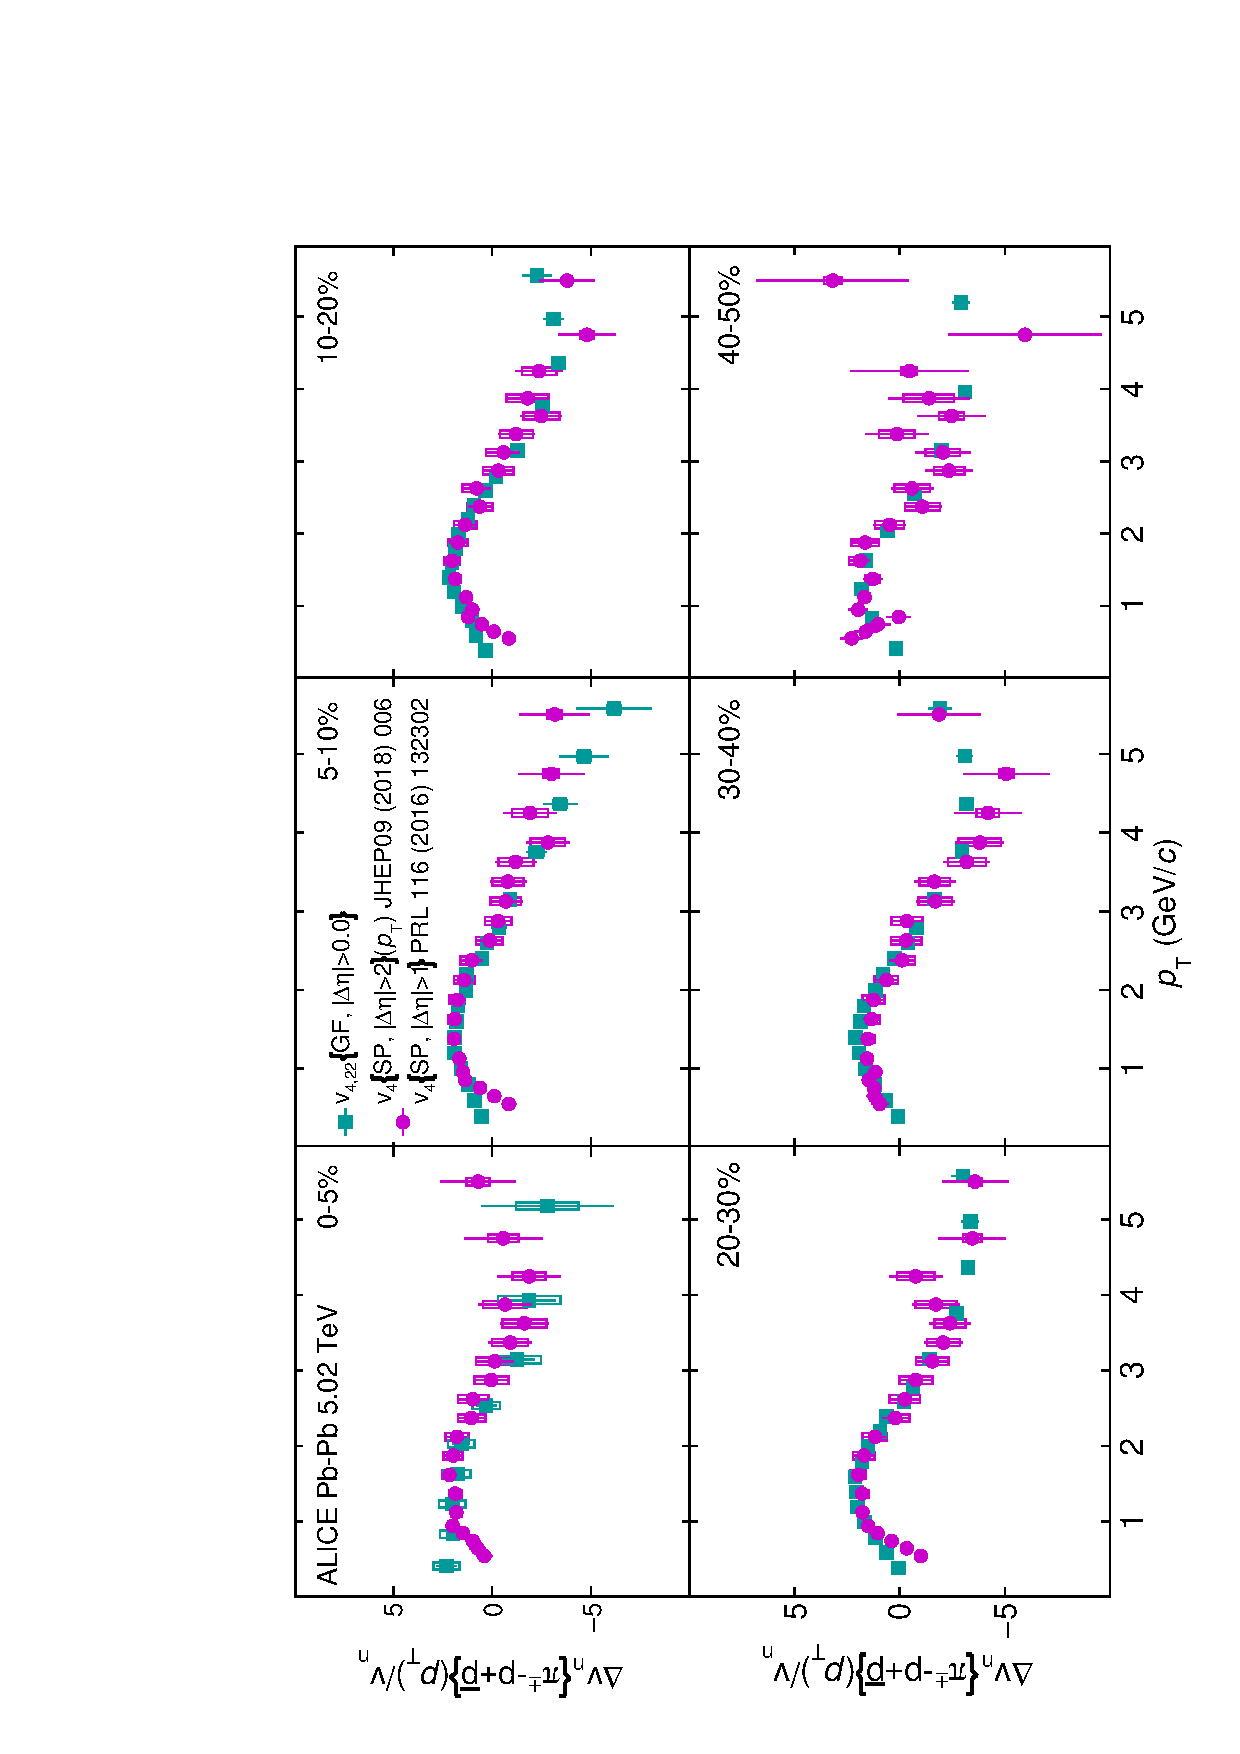
\includegraphics[scale=0.6]{figures/results/massOrdering_vn_pion_proton_to_charged.pdf}
\end{center}
\caption{The comparison between $[v_{4,22}^{\pi^{\pm}} -  v_{4,22}^{\rm p+\bar{p}}](p_{\rm T}) / v_{4,22}^{\rm h^{\pm}} $ and $[v_{4}^{\pi^{\pm}} -  v_{4}^{\rm p+\bar{p}}](p_{\rm T}) / v_{4}^{\rm h^{\pm}} $  grouped into different centrality intervals of Pb--Pb collisions at \sNN.}
\label{massOrderingComparison}
\end{figure}


%$\frac{\Delta v_{4,22}^{\pi^{\pm}}-v_{4,22}^{p+\bar{p}}$(p_{rm T})}{v_{4,22}^{h^{\pm}}}$

\newpage
\subsection{Comparison with models}
\label{SubSec:hydro}
%Measurements of anisotropic flow coefficients, $v_{n}$, at RHIC and the LHC are described well by hydrodynamic calculations \cite{Xu:2016hmp, McDonald:2016vlt, Zhao:2017yhj}. 

The comparison of various anisotropic flow measurements and hydrodynamic calculations have been presented and discussed in great details in \cite{Xu:2016hmp, McDonald:2016vlt, Zhao:2017yhj}. A recent comparison between $v_{n}$ measurements reported by ALICE \cite{Acharya:2018zuq} and two hydrodynamic calculations from \cite{Zhao:2017yhj} shed new light on the initial conditions and the transport properties of the created system in Pb--Pb collisions. Both hydrodynamic calculations are based on iEBE-VISHNU \cite{Shen:2014vra}, an event-by-event version of the VISHNU hybrid model \cite{Song:2010aq} coupling $2+1$~dimensional viscous hydrodynamics (VISH2+1) \cite{Song:2007fn} to a hadronic cascade model (UrQMD). The initial conditions used for these calculations are described by AMPT \cite{Lin:2004en} and TRENTo \cite{Moreland:2014oya}, both with $\tau_{0}$=0.6 fm/$c$ and $T_{sw}$ =148 MeV \cite{Bernhard:2016tnd}. For AMPT initial conditions, constant values of specific shear viscosity ($\eta/s =0.08$, the lower limit conjectured by AdS/CFT) and bulk viscosity ($\zeta/s = 0$) are utilised. The version of the model that uses TRENTo \cite{Moreland:2014oya} initial conditions incorporates a temperature dependent specific shear and bulk viscosity extracted from the global bayesian analysis \cite{Bernhard:2016tnd}. \footnote{ For simplicity in the rest of this article the model with AMPT initial conditions, $\eta/s =0.08$ and $\zeta/s =0$ is referred to as AMPT and the model with TRENTo initial conditions, $\eta/s(\rm{T})$ and $\zeta/s(\rm{T})$ is referred to as TRENTo.} 

The comparison between $v_{n}$ measurements and these two hydrodynamic calculations illustrates a qualitative agreement. This agreement between the data and the models depends on the particle species, transverse momentum range and centrality percentile. Overall, the AMPT model reproduces these measurements more accurately than the TRENTo model \cite{Acharya:2018zuq}. In order to further investigate the performance of these two models in reproducing $v_{n}$ measurements, the relative ratios between each model and the measurements of \pion, \kaon~and \proton~have been obtained. Table \ref{ModelDataComparisonflow} summarises these relative ratios. The values represent the ranges across all centralities that each model is able to describe the measurements of $v_n$ for each particle species. Comparison between the performance of the two models shows that the AMPT calculations reproduce $v_{2}$ slightly better that TRENTo\DIFdelbegin \DIFdel{with $\sim3\%$}\DIFdelend . Both models reproduce \DIFaddbegin \DIFadd{the }\DIFaddend $v_{3}$ measurements relatively better than $v_{2}$, however AMPT performs better \DIFdelbegin \DIFdel{that TRENTowith $\sim10\%$ }\DIFdelend \DIFaddbegin \DIFadd{than TRENTo}\DIFaddend . Finally, the comparison between the models and $v_{4}$ measurements show that AMPT has an absolute better performance \DIFdelbegin \DIFdel{up to $\sim17\%$ }\DIFdelend compared to TRENTo. These values should be taken with caution as $v_{4}$ has larger uncertainties with respect to $v_{3}$ and $v_{2}$. 

\begin{table}[!h]
\centering
\resizebox{0.81\textwidth}{!}{\begin{tabular}{ |p{4.5cm} |l|c|c|c|c|c|c|c|c|c|}
\hline
\multicolumn{1}{| c |}{} & \multicolumn{3}{| c |}{ $v_{2}$ } & \multicolumn{3}{| c |}{ $v_{3}$} & \multicolumn{3}{| c |}{ $v_{4}$}  \\
\hline
Error source  & \pion &  \kaon & \proton &  \pion & \kaon & \proton &  \pion &  \kaon & \proton \\ \hline  \hline
AMPT calculations & 3-13\% & 0-16\% & 0-20\% & 0-8\% & 5-12\% & 0-4\%& 6-12\% & 5-12\% & 0-4\%  \\
TRENTo calculations & 6-17\% & 0-19\% & 3-19\% & 2-15\% & 7-22\% & 0-11\% & 7-25\% & 16-28\% & 0-21\% \\
 \hline
\end{tabular}}

\caption{List of minimum and maximum value of the fit to relative ratios between the data and each model for  $v_{n} (n=2,3,4)$ of \pion, \kaon~and \proton. The minimum and maximum are obtained from 0-5\% up to 40-50\% centrality intervals .}\label{ModelDataComparisonflow}
\end{table}

\begin{table}[!h]
\resizebox{\textwidth}{!}{\begin{tabular}{ |p{4.5cm} |l|c|c|c|c|c|c|c|c|c|c|c|c|}
\hline
\multicolumn{1}{| c |}{} & \multicolumn{3}{| c |}{ $v_{4,22}$ } & \multicolumn{3}{| c |}{ $v_{5,32}$} & \multicolumn{3}{| c |}{ $v_{6,33}$} & \multicolumn{3}{| c |}{ $v_{6,222}$} \\
\hline
Error source  & \pion &  \kaon & \proton &  \pion & \kaon & \proton &  \pion &  \kaon & \proton &  \pion &  \kaon & \proton \\ \hline  \hline
AMPT claculations &  5-32\% & 2-30\%  & 3-30\% & 3-28\%  & 5-29\% &  1-65\% & 0-46\% & 0-46\% & 0-97\% & 6-52\% & 0-80\%  & 0-118\% \\
TRENTo calculations & 0-30\% & 4-33\% & 0-21\% &  24-49\% & 33-97\% & 12-58\% & 0-43\% & 0-46\% & 0-95\% & 0-20\% & 0-34\% & 0-78\%\\
 \hline
\end{tabular}}
\caption{List of minimum and maximum value of the fit to relative ratios between the data and each model for  $v_{n,mk}$ of \pion, \kaon~and \proton. The minimum and maximum are obtained from 0-10\% up to 50-60\% (40-50\% for $v_{6,33}$) centrality intervals .}\label{ModelDataComparisonNLflow}
\end{table}

%Recently, it was shown that the \pT-integrated non-linear flow modes are good observables to constrain the initial conditions and transport properties of the system \cite{Acharya:2017zfg}. 
%To test the validity of these hydrodynamic models a comparison is performed between the measured non-linear flow modes and two hydrodynamical calculations from \cite{Zhao:2017yhj}.  Both calculations are based on iEBE-VISHNU \cite{Shen:2014vra}, an event-by-event version of the VISHNU hybrid model \cite{Song:2010aq} coupling $2+1$~dimensional viscous hydrodynamics (VISH2+1) \cite{Song:2007fn} to a hadronic cascade model (UrQMD). One of these models uses AMPT \cite{Lin:2004en} initial conditions with constant values of specific shear viscosity ($\eta/s =0.08$, the lower limit conjectured by AdS/CFT) and bulk viscosity ($\zeta/s = 0$), and the other model incorporates TRENTo \cite{Moreland:2014oya} initial conditions with a temperature dependent specific shear and bulk viscosity. Both calculations are based on iEBE-VISHNU \cite{Shen:2014vra}, an event-by-event version of the VISHNU hybrid model \cite{Song:2010aq} coupling $2+1$~dimensional viscous hydrodynamics (VISH2+1) \cite{Song:2007fn} to a hadronic cascade model (UrQMD). One of these models uses AMPT \cite{Lin:2004en} initial conditions with constant values of specific shear viscosity ($\eta/s =0.08$, the lower limit conjectured by AdS/CFT) and bulk viscosity ($\zeta/s = 0$), and the other model incorporates TRENTo \cite{Moreland:2014oya} initial conditions with a temperature dependent specific shear and bulk viscosity. 

To achieve additional constraints on the initial conditions and transport properties of the system and test the validity of these hydrodynamic models, a comparison is performed between the measured \pT-dependent non-linear flow modes for \pion, \kaon, \proton, \Ks~and \lambdas~with the same two hydrodynamical calculations reported in \cite{Zhao:2017yhj}. Figures \ref{v422_model}-\ref{v6222_model} present the comparison between the measurements and two model predictions for the \pT-differential $v_{4,22}$, $v_{5,32}$, $v_{6,33}$ and $v_{6,222}$, respectively, for \pion, \kaon~and \proton~and Figs. \ref{v422_model_KL}-\ref{v633_model_KL} present these comparisons for the \pT-differential $v_{4,22}$, $v_{5,32}$ and $v_{6,33}$ for \Ks~and \lambdas~at 0-10\% up to 50-60\% centrality interval (40-50\% centrality interval for $v_{6,33}$) of Pb--Pb collisions at \sNN. The solid bands show the AMPT model and the hatched bands represent the TRENTo calculations. The bottom panels in each plot in Figs. \ref{v422_model}-\ref{v633_model_KL} present the difference between the models and the measurement. Both TRENTo and AMPT models produce the mass ordering feature at $p_{\rm{T}}<2.5$ \GeV~for all non-linear flow modes. In particular, the comparison between the models and the measurements of $v_{4,22}$ reveals that TRENTo reproduces the data very well from 0-10\% up to 30-40\% centrality interval and fails to reproduce the measurements for the remaining more peripheral centrality intervals. On the other hand, AMPT overestimates the measurements from 0-10\% up to 30-40\% centrality interval. At 40-50\% centrality interval, it reproduces \DIFaddbegin \DIFadd{the }\DIFaddend measurements for all particle species except \pion, where it slightly underestimates the results. For more peripheral collisions, it reproduces the \kaon, \proton~and \lambdas~measurements and underestimates the results for \pion~and \Ks. 

In a similar attempt to \DIFaddbegin \DIFadd{comparison between the }\DIFaddend $v_{n}$ \DIFdelbegin \DIFdel{data-model comparison }\DIFdelend \DIFaddbegin \DIFadd{measurement and the model calculation }\DIFaddend in Tab. \ref{ModelDataComparisonflow}, the performance of these models have been further studied for $v_{n,mk}$ by taking the relative ratios between each model and the measurements of \pion, \kaon~and \proton. These relative ratios are summarised in Tab. \ref{ModelDataComparisonNLflow} where TRENTo calculations reproduce $v_{4,22}$ slightly better than AMPT\DIFdelbegin \DIFdel{with $\sim2\%$}\DIFdelend . Comparison between Tab. \ref{ModelDataComparisonNLflow} and \ref{ModelDataComparisonflow} shows that the AMPT calculations reproduces $v_{4,22}$ with $\sim$20\% higher discrepancy on average compared to $v_{4}$, and, TRENTo calculations performs \DIFdelbegin \DIFdel{slightly better in }\DIFdelend \DIFaddbegin \DIFadd{equally well for }\DIFaddend $v_{4,22}$ compared to $v_{4}$\DIFdelbegin \DIFdel{with $2-7\%$}\DIFdelend . It is necessary to stress \DIFaddbegin \DIFadd{however }\DIFaddend that the non-linear flow modes have smaller magnitudes with respect to $v_{n}$ and any discrepancy between the models and the data becomes magnified in the ratios reported in Tab. \ref{ModelDataComparisonNLflow}. 


%Comparison between the performance of the two models shows that the AMPT calculations reproduce $v_{2}$ slightly better that TRENTo with $\sim3\%$. Both models reproduce $v_{3}$ measurements better, however AMPT performs better with up to $\sim10\%$. Finally, the comparison between the models and $v_{4}$ measurements show that AMPT has an absolute better performance up to $\sim17\%$ compared to TRENTo. These values should be taken with caution as $v_{4}$ has larger uncertainties with respect to $v_{3}$ and $v_{2}$. 


%In order to compare their performance in describing the $v_4$ and $v_{4,22}$ measurements, the relative ratios between each model and the measurements of \pion, \kaon~and \proton~have been obtained also for $v_{4,22}$. Table \ref{ModelDataComparisonNLflow} summarises these relative ratios for $v_{n,mk}$. Comparison between 


%Comparison between Tab. \ref{ModelDataComparisonNLflow} and \ref{ModelDataComparisonflow} shows that the AMPT calculations reproduces $v_{4,22}$ with $\sim$20\% higher discrepancy on average compared to $v_{4}$, while, TRENTo calculations performs better in $v_{4,22}$ compared to $v_{4}$ with $\sim$7\%.  

%These values should be taken with caution as the non-linear flow modes have smaller magnitude and any discrepancy between the models and the data becomes magnified in the ratios.



For $v_{5,32}$, the \DIFdelbegin \DIFdel{comparisons seem }\DIFdelend \DIFaddbegin \DIFadd{comparison seems }\DIFaddend slightly different where TRENTo predictions overestimate the measurements for all centrality intervals\DIFdelbegin \DIFdel{. While }\DIFdelend \DIFaddbegin \DIFadd{, while }\DIFaddend AMPT seemingly reproduces the data better. \DIFdelbegin \DIFdel{AMPT }\DIFdelend \DIFaddbegin \DIFadd{The AMPT model }\DIFaddend slightly overestimates the measurements from 0-10\% to 20-30\% centrality interval. It underestimates the measurements of \pion, \kaon~and \proton~for more peripheral collisions while it reproduces the measurements of \Ks~and \lambdas~relatively well up to 40-50\% centrality interval. These comparisons are reflected in Table \ref{ModelDataComparisonNLflow} where AMPT performs on average $20-27\%$ better than TRENTo for \pion, \kaon~and \proton. 

For $v_{6,33}$, both models reproduce the data at 0-10\% centrality interval. For 10-20\% up to 30-40\% centrality interval, AMPT reproduces the data while TRENTo slightly overestimates the measurements. Finally, comparison with $v_{6,222}$ shows an agreement between both models and the measurements of \pion, \kaon~and \proton~at 0-10\% up to 30-40\% centrality intervals  \footnote{The ratios reported for $v_{6,33}$ and $v_{6,222}$ in Tab. \ref{ModelDataComparisonNLflow} are not to be taken at face value as the magnitudes of these two non-linear flow modes are almost zero.}. 


 \begin{figure}[h]
\begin{center}
\includegraphics[scale=0.73]{figures/model/TrentoAndAMPT_v422_gap00_PID2.pdf}
\end{center}
\caption{The \pT-differential $v_{4,22}$ for \pion, \kaon~and \proton~in 0-10\% up to 50-60\% centrality intervals of Pb--Pb collisions at \sNN compared with iEBE-VISHNU hybrid models with two different sets of initial parameters: AMPT initial conditions ($\eta/s$= 0.08 and $\zeta/s$ = 0) shown in solid bands and TRENTo initial conditions ($\eta/s({\rm T})$ and $\zeta/s({\rm T})$) in hatched bands. The bottom panels show the difference between the measurements and each model.}
\label{v422_model}
\end{figure}

\begin{figure}[h]
\begin{center}
\includegraphics[scale=0.73]{figures/model/TrentoAndAMPT_v523_gap00_PID2.pdf}
\end{center}
\caption{The \pT-differential $v_{5,32}$ for \pion, \kaon~and \proton~in 0-10\% up to 50-60\% centrality intervals of Pb--Pb collisions at \sNN compared with iEBE-VISHNU hybrid models with two different sets of initial parameters: AMPT initial conditions ($\eta/s$= 0.08 and $\zeta/s$ = 0) shown in solid bands and TRENTo initial conditions ($\eta/s({\rm T})$ and $\zeta/s({\rm T})$) in hatched bands. The bottom panels show the difference between the measurements and each model.}
\label{v523_model}
\end{figure}


\begin{figure}[h]
\begin{center}
\includegraphics[scale=0.73]{figures/model/TrentoAndAMPT_v633_gap00_PID2.pdf}
\end{center}
\caption{The \pT-differential $v_{6,33}$ for \pion, \kaon~and \proton~in 0-10\% up to 40-50\% centrality intervals of Pb--Pb collisions at \sNN compared with iEBE-VISHNU hybrid models with two different sets of initial parameters: AMPT initial conditions ($\eta/s$= 0.08 and $\zeta/s$ = 0) shown in solid bands and TRENTo initial conditions ($\eta/s({\rm T})$ and $\zeta/s({\rm T})$) in hatched bands. The bottom panels show the difference between the measurements and each model.}
\label{v633_model}
\end{figure}

\begin{figure}[h]
\begin{center}
\includegraphics[scale=0.73]{figures/model/TrentoAndAMPT_v6222_gap00_PID2.pdf}
\end{center}
\caption{The \pT-differential $v_{6,222}$ for \pion, \kaon~and \proton~in 0-10\% up to 50-60\% centrality intervals of Pb--Pb collisions at \sNN compared with iEBE-VISHNU hybrid models with two different sets of initial parameters: AMPT initial conditions ($\eta/s$= 0.08 and $\zeta/s$ = 0) shown in solid bands and TRENTo initial conditions ($\eta/s({\rm T})$ and $\zeta/s({\rm T})$) in hatched bands. The bottom panels show the difference between the measurements and each model.}
\label{v6222_model}
\end{figure}



 \begin{figure}[h]
\begin{center}
\includegraphics[scale=0.73]{figures/model/TrentoAndAMPT_v422_gap00_LambdaK0s.pdf}
\end{center}
\caption{The \pT-differential $v_{4,22}$ for \Ks~and \lambdas~in 0-10\% up to 50-60\% centrality intervals of Pb--Pb collisions at \sNN compared with iEBE-VISHNU hybrid models with two different sets of initial parameters: AMPT initial conditions ($\eta/s$= 0.08 and $\zeta/s$ = 0) shown in solid bands and TRENTo initial conditions ($\eta/s({\rm T})$ and $\zeta/s({\rm T})$) in hatched bands. The bottom panels show the difference between the measurements and each model.}
\label{v422_model_KL}
\end{figure}


 \begin{figure}[h]
\begin{center}
\includegraphics[scale=0.73]{figures/model/TrentoAndAMPT_v523_gap00_LambdaK0s.pdf}
\end{center}
\caption{The \pT-differential $v_{5,32}$ for \Ks~and \lambdas~in 0-10\% up to 50-60\% centrality intervals of Pb--Pb collisions at \sNN compared with iEBE-VISHNU hybrid models with two different sets of initial parameters: AMPT initial conditions ($\eta/s$= 0.08 and $\zeta/s$ = 0) shown in solid bands and TRENTo initial conditions ($\eta/s({\rm T})$ and $\zeta/s({\rm T})$) in hatched bands. The bottom panels show the difference between the measurements and each model.}
\label{v523_model_KL}
\end{figure}


 \begin{figure}[h]
\begin{center}
\includegraphics[scale=0.73]{figures/model/TrentoAndAMPT_v633_gap00_LambdaK0s.pdf}
\end{center}
\caption{The \pT-differential $v_{6,33}$ for \Ks~and \lambdas~in 0-10\% up to 40-50\% centrality intervals of Pb--Pb collisions at \sNN compared with iEBE-VISHNU hybrid models with two different sets of initial parameters: AMPT initial conditions ($\eta/s$= 0.08 and $\zeta/s$ = 0) shown in solid bands and TRENTo initial conditions ($\eta/s({\rm T})$ and $\zeta/s({\rm T})$) in hatched bands. The bottom panels show the difference between the measurements and each model.}
\label{v633_model_KL}
\end{figure}


All in all, this study shows larger difference between the model calculations and \DIFaddbegin \DIFadd{the }\DIFaddend $v_{n,mk}$ measurements with respect to that of $v_{n}$, indicating a larger sensitivity to the initial conditions and transport properties \DIFdelbegin \DIFdel{in }\DIFdelend \DIFaddbegin \DIFadd{for the }\DIFaddend non-linear flow modes. As a result, it is useful to tune the input parameters of hydrodynamic models \DIFdelbegin \DIFdel{using }\DIFdelend \DIFaddbegin \DIFadd{considering also }\DIFaddend the non-linear flow measurements\DIFdelbegin \DIFdel{and constrain the values of transport properties and the initial conditions of the system. }\DIFdelend \DIFaddbegin \DIFadd{. %DIF >  and constrain the values of transport properties and the initial conditions of the system.
}\DIFaddend 

%All in all, comparing this effort to the data-model comparison for anisotropic flow coefficients \cite{Acharya:2018zuq} shows that non-linear modes are more sensitive to the initial conditions and transport properties. However, similar to model-data comparisons for anisotropic flow, neither of the models can reproduce the data for all centrality intervals and particle species. As a result, in order to constrain the values of transport properties and the initial conditions of the system, it is necessary to tune the input parameters of hydrodynamic models using these measurements.






\newpage
\newpage

\section{Summary}
\label{Sec:conclusion}

In this article, the measurement of non-linear flow modes, $v_{4,22}$, $v_{5,32}$, $v_{6,222}$ and $v_{6,33}$ as a function of transverse momentum for different particle species, i.e. \pion, \kaon, \Ks, \proton, \lambdas~and $\phi$-meson are reported for the first time. The results are presented in a wide range of centrality intervals from 0-5\% up to 50-60\% in Pb--Pb collisions at \sNN. The magnitude of non-linear flow modes, $v_{n,mk}$, are obtained with a multi-particle correlation technique, namely the generic framework, selecting the identified hadron under study and the reference flow particles from different, non-overlapping pseudorapidity regions.  

The \DIFdelbegin \DIFdel{measurements of }\DIFdelend \DIFaddbegin \DIFadd{measured }\DIFaddend $v_{4,22}$, $v_{5,32}$ and $v_{6,222}$ exhibit a \DIFdelbegin \DIFdel{clear }\DIFdelend \DIFaddbegin \DIFadd{distinct }\DIFaddend centrality dependence. This centrality dependence originates from the contribution of initial state eccentricity, $\varepsilon_{2}$, as shown in Eq. \ref{Eq:V4V5V6}. As expected, $v_{6,33}$ does not exhibit a considerable centrality dependence since $\varepsilon_{3}$ quantifies primarily the event-by-event fluctuations of the initial energy density profile. This is supported by the relatively large magnitude of $v_{6,33}$ in the most-central collisions (0-5\%). A clear mass ordering is observed in the low \pT~region (\pT$< 2.5$ \GeV). A closer comparison between $v_{4}$ and $v_{4,22}$ shows that this mass ordering seems slightly larger for $v_{4,22}$ than $v_{4}$ at very low \pT~(\pT<0.8 \GeV). \DIFdelbegin \DIFdel{At higher }%DIFDELCMD < \pT%%%
\DIFdel{~values ($0.8<$}%DIFDELCMD < \pT%%%
\DIFdel{$< 2.5$ }%DIFDELCMD < \GeV%%%
\DIFdel{), the mass ordering is similar to observations in $v_{4}$ which is associated with the interplay between the anisotropic flow and radial flow. }\DIFdelend %DIF > At higher \pT~values ($0.8<$\pT$< 2.5$ \GeV), the mass ordering is similar to observations in $v_{4}$ which is associated with the interplay between the anisotropic and radial flow. 
In the intermediate \pT~region (\pT$> 2.5$ \GeV), a particle type grouping is observed where the magnitude of non-linear modes for baryons are larger than for mesons similar to observations in $v_{n}$ measurements. The NCQ scaling holds at an approximate level of $\pm 20$\% within the current level of statistical and systematic uncertainties, similar to that of anisotropic flow coefficients \cite{Acharya:2018zuq}. 

The comparison of two models based on the iEBE-VISHNU hybrid model, and with two different initial conditions (AMPT and TRENTo) and transport properties show that neither of the models are able to fully describe the measurements. This varies depending on the centrality percentile and particle species similar to the model-data comparison for anisotropic flow \DIFaddbegin \DIFadd{coefficients }\DIFaddend \cite{Acharya:2018zuq}. Measurements are better predicted by the models in more central collisions. All in all, the model using AMPT initial conditions ($\eta/s = 0.08$ and $\zeta/s =0$) exhibits a magnitude and shape closer to the measurements. As a result, in order to further constrain the values of transport properties and the initial conditions of the system, it is necessary to tune the input parameters of future hydrodynamic calculations attempting to describe these measurements.
%\section{Additional figures}

\subsection{$\rm{KE_{T}}$ scaling}
\label{Subsubsection:KETscaling}

One suggestion to further study the scaling properties of flow coefficients was to extend the scaling to lower \pT~values by studying the transverse kinetic energy dependence of anisotropic flow harmonics. Transverse kinetic energy is defined as ${\rm KE}_{\rm{T}} = m_{\rm{T}} - m_{\rm{0}}$, where $m_{\rm{T}}= \sqrt{m_{0}^2 + p_{\rm{T}}^2}$ is the transverse mass. Figures \ref{v422_KET}, \ref{v523_KET}, \ref{v633_KET} and \ref{v6222_KET} present ${\rm KE}_{\rm{T}}$ scaling for $v_{4,22}$, $v_{5,32}$, $v_{6,33}$ and $v_{6,222}$ respectively, for \pion, \kaon, \proton, \Ks, \lambdas~and $\phi$-meson grouped in different centrality intervals.

\begin{figure}[htb]
\begin{center}
\includegraphics[scale=0.82]{figures/scaling/All_v422_gap00_KET_3by3.pdf}

\end{center}
\caption{The $(m_{\rm{T}} - m_{0})/n_{q}$-dependence of $v_{4,22}/n_{q}$ for different particle species grouped into different centrality intervals of Pb--Pb collisions \sNN. Statistical and systematic uncertainties are shown as bars and boxes, respectively. It is seen that the $\rm KE_{T}$ scaling holds for $v_{4,22}$ at an approximate level.}
\label{v422_KET}
\end{figure}

\begin{figure}[htb]
\begin{center}
\includegraphics[scale=0.82]{figures/scaling/All_v523_gap00_KET_3by3.pdf}
\end{center}
\caption{The $(m_{\rm{T}} - m_{0})/n_{q}$-dependence of $v_{5,32}/n_{q}$ for different particle species grouped into different centrality intervals of Pb--Pb collisions \sNN. Statistical and systematic uncertainties are shown as bars and boxes, respectively. It is seen that the $\rm KE_{T}$ scaling holds for $v_{5,32}$ at an approximate level.}
\label{v523_KET}
\end{figure}

\begin{figure}[htb]
\begin{center}
\includegraphics[scale=0.82]{figures/scaling/All_v633_gap00_KET_3by2.pdf}
\end{center}
\caption{The $(m_{\rm{T}} - m_{0})/n_{q}$-dependence of $v_{6,33}/n_{q}$ for different particle species grouped into different centrality intervals of Pb--Pb collisions \sNN. Statistical and systematic uncertainties are shown as bars and boxes, respectively. It is seen that the $\rm KE_{T}$ scaling holds for $v_{6,33}$ at an approximate level.}
\label{v633_KET}
\end{figure}

\begin{figure}[htb]
\begin{center}
\includegraphics[scale=0.82]{figures/scaling/All_v6222_gap00_KET_3by3.pdf}
\end{center}
\caption{The $(m_{\rm{T}} - m_{0})/n_{q}$-dependence of $v_{6,222}/n_{q}$ for different particle species grouped into different centrality intervals of Pb--Pb collisions \sNN. Statistical and systematic uncertainties are shown as bars and boxes, respectively. It is seen that the $\rm KE_{T}$ scaling holds for $v_{6,222}$ at an approximate level.}
\label{v6222_KET}
\end{figure}

%%%%%%%%%%%%%%%%%%%%%%%%%%%%%%%%
% end main text 
%%%%%%%%%%%%%%%%%%%%%%%%%%%%%%%%

%%%%% acknowledgements - handled by EB chairs 
\newenvironment{acknowledgement}{\relax}{\relax}
\begin{acknowledgement}
\section*{Acknowledgements}
% add specific acknowledgements here 
% ...but please don't remove the line below: funding agencies
% will be acknowledged with a custom tex file handled by EB chairs after Collab Round 2
%\input{acknowledgements.tex}
\end{acknowledgement}

\newpage

%%%%%%%% Bibliography 
\bibliographystyle{utphys}   % Remember we use title in the biblio
\providecommand{\href}[2]{#2}\begingroup\raggedright\begin{thebibliography}{10}

\bibitem{Borsanyi:2010cj}
S.~Borsanyi, G.~Endrodi, Z.~Fodor, A.~Jakovac, S.~D. Katz, S.~Krieg, C.~Ratti,
  and K.~K. Szabo, ``{The QCD equation of state with dynamical quarks}'',
  \href{http://dx.doi.org/10.1007/JHEP11(2010)077}{{\em JHEP} {\bfseries 11}
  (2010) },
\href{http://arxiv.org/abs/1007.2580}{{\ttfamily arXiv:1007.2580 [hep-lat]}}.
%%CITATION = ARXIV:1007.2580;%%.

\bibitem{Bhattacharya:2014ara}
T.~Bhattacharya {\em et~al.}, ``{QCD Phase Transition with Chiral Quarks and
  Physical Quark Masses}'',
  \href{http://dx.doi.org/10.1103/PhysRevLett.113.082001}{{\em Phys. Rev.
  Lett.} {\bfseries 113} no.~8, (2014) },
\href{http://arxiv.org/abs/1402.5175}{{\ttfamily arXiv:1402.5175 [hep-lat]}}.
%%CITATION = ARXIV:1402.5175;%%.

\bibitem{Shuryak:1984nq}
E.~V. Shuryak, ``{Theory and phenomenology of the QCD vacuum}'',
\href{http://dx.doi.org/10.1016/0370-1573(84)90037-1}{{\em Phys. Rept.}
  {\bfseries 115} (1984) }.
%%CITATION = PRPLC,115,151;%%.

\bibitem{Cleymans:1985wb}
J.~Cleymans, R.~V. Gavai, and E.~Suhonen, ``{Quarks and Gluons at High
  Temperatures and Densities}'',
\href{http://dx.doi.org/10.1016/0370-1573(86)90169-9}{{\em Phys. Rept.}
  {\bfseries 130} (1986) }.
%%CITATION = PRPLC,130,217;%%.

\bibitem{Bass:1998vz}
S.~A. Bass, M.~Gyulassy, H.~Stoecker, and W.~Greiner, ``{Signatures of quark
  gluon plasma formation in high-energy heavy ion collisions: A Critical
  review}'', \href{http://dx.doi.org/10.1088/0954-3899/25/3/013}{{\em J. Phys.}
  {\bfseries G25} (1999) },
\href{http://arxiv.org/abs/hep-ph/9810281}{{\ttfamily arXiv:hep-ph/9810281
  [hep-ph]}}.
%%CITATION = HEP-PH/9810281;%%.

\bibitem{Miller:2003kd}
M.~Miller and R.~Snellings, ``{Eccentricity fluctuations and its possible
  effect on elliptic flow measurements}'',
\href{http://arxiv.org/abs/nucl-ex/0312008}{{\ttfamily arXiv:nucl-ex/0312008
  [nucl-ex]}}.
%%CITATION = NUCL-EX/0312008;%%.

\bibitem{Bhalerao:2006tp}
R.~S. Bhalerao and J.-Y. Ollitrault, ``{Eccentricity fluctuations and elliptic
  flow at RHIC}'', \href{http://dx.doi.org/10.1016/j.physletb.2006.08.055}{{\em
  Phys. Lett.} {\bfseries B641} (2006) },
\href{http://arxiv.org/abs/nucl-th/0607009}{{\ttfamily arXiv:nucl-th/0607009
  [nucl-th]}}.
%%CITATION = NUCL-TH/0607009;%%.

\bibitem{Alver:2008zza}
B.~Alver {\em et~al.}, ``{Importance of correlations and fluctuations on the
  initial source eccentricity in high-energy nucleus-nucleus collisions}'',
  \href{http://dx.doi.org/10.1103/PhysRevC.77.014906}{{\em Phys. Rev.}
  {\bfseries C77} (2008) },
\href{http://arxiv.org/abs/0711.3724}{{\ttfamily arXiv:0711.3724 [nucl-ex]}}.
%%CITATION = ARXIV:0711.3724;%%.

\bibitem{Alver:2010gr}
B.~Alver and G.~Roland, ``{Collision geometry fluctuations and triangular flow
  in heavy-ion collisions}'',
  \href{http://dx.doi.org/10.1103/PhysRevC.82.039903,
  10.1103/PhysRevC.81.054905}{{\em Phys. Rev.} {\bfseries C81} (2010) },
  \href{http://arxiv.org/abs/1003.0194}{{\ttfamily arXiv:1003.0194 [nucl-th]}}.
[Erratum: Phys. Rev.C82,039903(2010)].
%%CITATION = ARXIV:1003.0194;%%.

\bibitem{Alver:2010dn}
B.~H. Alver, C.~Gombeaud, M.~Luzum, and J.-Y. Ollitrault, ``{Triangular flow in
  hydrodynamics and transport theory}'',
  \href{http://dx.doi.org/10.1103/PhysRevC.82.034913}{{\em Phys. Rev.}
  {\bfseries C82} (2010) },
\href{http://arxiv.org/abs/1007.5469}{{\ttfamily arXiv:1007.5469 [nucl-th]}}.
%%CITATION = ARXIV:1007.5469;%%.

\bibitem{Manly:2005zy}
{\bfseries PHOBOS} Collaboration, S.~Manly {\em et~al.}, ``{System size, energy
  and pseudorapidity dependence of directed and elliptic flow at RHIC}'',
  \href{http://dx.doi.org/10.1016/j.nuclphysa.2006.06.079}{{\em Nucl. Phys.}
  {\bfseries A774} (2006) },
\href{http://arxiv.org/abs/nucl-ex/0510031}{{\ttfamily arXiv:nucl-ex/0510031
  [nucl-ex]}}.
%%CITATION = NUCL-EX/0510031;%%.

\bibitem{Voloshin:2006gz}
S.~A. Voloshin, ``{Toward the energy and the system size dependece of elliptic
  flow: Working on flow fluctuations}'', in {\em {22nd Winter Workshop on
  Nuclear Dynamics (WWND 2006) La Jolla, California, March 11-19, 2006}}.
\newblock 2006.
\newblock
\href{http://arxiv.org/abs/nucl-th/0606022}{{\ttfamily arXiv:nucl-th/0606022
  [nucl-th]}}.
\newblock
%%CITATION = NUCL-TH/0606022;%%.

\bibitem{Voloshin:1994mz}
S.~Voloshin and Y.~Zhang, ``{Flow study in relativistic nuclear collisions by
  Fourier expansion of Azimuthal particle distributions}'',
  \href{http://dx.doi.org/10.1007/s002880050141}{{\em Z. Phys.} {\bfseries C70}
  (1996) },
\href{http://arxiv.org/abs/hep-ph/9407282}{{\ttfamily arXiv:hep-ph/9407282
  [hep-ph]}}.
%%CITATION = HEP-PH/9407282;%%.

\bibitem{Adams:2003am}
{\bfseries STAR} Collaboration, J.~Adams {\em et~al.}, ``{Particle type
  dependence of azimuthal anisotropy and nuclear modification of particle
  production in Au + Au collisions at $\sqrt{s_{NN}} = $200~GeV}'',
  \href{http://dx.doi.org/10.1103/PhysRevLett.92.052302}{{\em Phys. Rev. Lett.}
  {\bfseries 92} (2004) },
\href{http://arxiv.org/abs/nucl-ex/0306007}{{\ttfamily arXiv:nucl-ex/0306007
  [nucl-ex]}}.
%%CITATION = NUCL-EX/0306007;%%.

\bibitem{Abelev:2007qg}
{\bfseries STAR} Collaboration, B.~I. Abelev {\em et~al.}, ``{Mass,
  quark-number, and $\sqrt{s_{NN}}$ dependence of the second and fourth flow
  harmonics in ultra-relativistic nucleus-nucleus collisions}'',
  \href{http://dx.doi.org/10.1103/PhysRevC.75.054906}{{\em Phys. Rev.}
  {\bfseries C75} (2007) },
\href{http://arxiv.org/abs/nucl-ex/0701010}{{\ttfamily arXiv:nucl-ex/0701010
  [nucl-ex]}}.
%%CITATION = NUCL-EX/0701010;%%.

\bibitem{Adler:2003kt}
{\bfseries PHENIX} Collaboration, S.~S. Adler {\em et~al.}, ``{Elliptic flow of
  identified hadrons in Au+Au collisions at $\sqrt{s_{NN}} = $200~GeV}'',
  \href{http://dx.doi.org/10.1103/PhysRevLett.91.182301}{{\em Phys. Rev. Lett.}
  {\bfseries 91} (2003) },
\href{http://arxiv.org/abs/nucl-ex/0305013}{{\ttfamily arXiv:nucl-ex/0305013
  [nucl-ex]}}.
%%CITATION = NUCL-EX/0305013;%%.

\bibitem{Adare:2006ti}
{\bfseries PHENIX} Collaboration, A.~Adare {\em et~al.}, ``{Scaling properties
  of azimuthal anisotropy in Au+Au and Cu+Cu collisions at s(NN) = 200-GeV}'',
  \href{http://dx.doi.org/10.1103/PhysRevLett.98.162301}{{\em Phys. Rev. Lett.}
  {\bfseries 98} (2007) },
\href{http://arxiv.org/abs/nucl-ex/0608033}{{\ttfamily arXiv:nucl-ex/0608033
  [nucl-ex]}}.
%%CITATION = NUCL-EX/0608033;%%.

\bibitem{Alver:2007qw}
{\bfseries PHOBOS} Collaboration, B.~Alver {\em et~al.}, ``{Event-by-Event
  Fluctuations of Azimuthal Particle Anisotropy in Au + Au Collisions at
  $\sqrt{s_{NN}}= 200$ GeV}'',
  \href{http://dx.doi.org/10.1103/PhysRevLett.104.142301}{{\em Phys. Rev.
  Lett.} {\bfseries 104} (2010) },
\href{http://arxiv.org/abs/nucl-ex/0702036}{{\ttfamily arXiv:nucl-ex/0702036
  [nucl-ex]}}.
%%CITATION = NUCL-EX/0702036;%%.

\bibitem{Adcox:2002ms}
{\bfseries PHENIX} Collaboration, K.~Adcox {\em et~al.}, ``{Flow measurements
  via two particle azimuthal correlations in Au+Au collisions at s(NN)**(1/2) =
  130-GeV}'', \href{http://dx.doi.org/10.1103/PhysRevLett.89.212301}{{\em Phys.
  Rev. Lett.} {\bfseries 89} (2002) },
\href{http://arxiv.org/abs/nucl-ex/0204005}{{\ttfamily arXiv:nucl-ex/0204005
  [nucl-ex]}}.
%%CITATION = NUCL-EX/0204005;%%.

\bibitem{Adamczyk:2013gw}
{\bfseries STAR} Collaboration, L.~Adamczyk {\em et~al.}, ``{Elliptic flow of
  identified hadrons in Au+Au collisions at $\sqrt{s_{NN}}=$ 7.7-62.4 GeV}'',
  \href{http://dx.doi.org/10.1103/PhysRevC.88.014902}{{\em Phys. Rev.}
  {\bfseries C88} (2013) },
\href{http://arxiv.org/abs/1301.2348}{{\ttfamily arXiv:1301.2348 [nucl-ex]}}.
%%CITATION = ARXIV:1301.2348;%%.

\bibitem{Adler:2004cj}
{\bfseries PHENIX} Collaboration, S.~S. Adler {\em et~al.}, ``{Saturation of
  azimuthal anisotropy in Au + Au collisions at s(NN)**(1/2) 62-GeV to
  200-GeV}'', \href{http://dx.doi.org/10.1103/PhysRevLett.94.232302}{{\em Phys.
  Rev. Lett.} {\bfseries 94} (2005) },
\href{http://arxiv.org/abs/nucl-ex/0411040}{{\ttfamily arXiv:nucl-ex/0411040
  [nucl-ex]}}.
%%CITATION = NUCL-EX/0411040;%%.

\bibitem{Afanasiev:2009wq}
{\bfseries PHENIX} Collaboration, S.~Afanasiev {\em et~al.}, ``{Systematic
  Studies of Elliptic Flow Measurements in Au+Au Collisions at s**(1/2) =
  200-GeV}'', \href{http://dx.doi.org/10.1103/PhysRevC.80.024909}{{\em Phys.
  Rev.} {\bfseries C80} (2009) },
\href{http://arxiv.org/abs/0905.1070}{{\ttfamily arXiv:0905.1070 [nucl-ex]}}.
%%CITATION = ARXIV:0905.1070;%%.

\bibitem{Adare:2011tg}
{\bfseries PHENIX} Collaboration, A.~Adare {\em et~al.}, ``{Measurements of
  Higher-Order Flow Harmonics in Au+Au Collisions at $\sqrt{s_{NN}} = 200$
  GeV}'', \href{http://dx.doi.org/10.1103/PhysRevLett.107.252301}{{\em Phys.
  Rev. Lett.} {\bfseries 107} (2011) },
\href{http://arxiv.org/abs/1105.3928}{{\ttfamily arXiv:1105.3928 [nucl-ex]}}.
%%CITATION = ARXIV:1105.3928;%%.

\bibitem{Ackermann:2000tr}
{\bfseries STAR} Collaboration, K.~H. Ackermann {\em et~al.}, ``{Elliptic flow
  in Au + Au collisions at (S(NN))**(1/2) = 130 GeV}'',
  \href{http://dx.doi.org/10.1103/PhysRevLett.86.402}{{\em Phys. Rev. Lett.}
  {\bfseries 86} (2001) },
\href{http://arxiv.org/abs/nucl-ex/0009011}{{\ttfamily arXiv:nucl-ex/0009011
  [nucl-ex]}}.
%%CITATION = NUCL-EX/0009011;%%.

\bibitem{Adler:2001nb}
{\bfseries STAR} Collaboration, C.~Adler {\em et~al.}, ``{Identified particle
  elliptic flow in Au + Au collisions at s(NN)**(1/2) = 130-GeV}'',
  \href{http://dx.doi.org/10.1103/PhysRevLett.87.182301}{{\em Phys. Rev. Lett.}
  {\bfseries 87} (2001) },
\href{http://arxiv.org/abs/nucl-ex/0107003}{{\ttfamily arXiv:nucl-ex/0107003
  [nucl-ex]}}.
%%CITATION = NUCL-EX/0107003;%%.

\bibitem{Adler:2002ct}
{\bfseries STAR} Collaboration, C.~Adler {\em et~al.}, ``{Azimuthal anisotropy
  and correlations in the hard scattering regime at RHIC}'',
  \href{http://dx.doi.org/10.1103/PhysRevLett.90.032301}{{\em Phys. Rev. Lett.}
  {\bfseries 90} (2003) },
\href{http://arxiv.org/abs/nucl-ex/0206006}{{\ttfamily arXiv:nucl-ex/0206006
  [nucl-ex]}}.
%%CITATION = NUCL-EX/0206006;%%.

\bibitem{Adler:2002pu}
{\bfseries STAR} Collaboration, C.~Adler {\em et~al.}, ``{Elliptic flow from
  two and four particle correlations in Au+Au collisions at $\sqrt{s_{NN}} =
  $130~GeV}'', \href{http://dx.doi.org/10.1103/PhysRevC.66.034904}{{\em Phys.
  Rev.} {\bfseries C66} (2002) },
\href{http://arxiv.org/abs/nucl-ex/0206001}{{\ttfamily arXiv:nucl-ex/0206001
  [nucl-ex]}}.
%%CITATION = NUCL-EX/0206001;%%.

\bibitem{Adams:2003zg}
{\bfseries STAR} Collaboration, J.~Adams {\em et~al.}, ``{Azimuthal anisotropy
  at RHIC: The First and fourth harmonics}'',
  \href{http://dx.doi.org/10.1103/PhysRevLett.92.062301}{{\em Phys. Rev. Lett.}
  {\bfseries 92} (2004) },
\href{http://arxiv.org/abs/nucl-ex/0310029}{{\ttfamily arXiv:nucl-ex/0310029
  [nucl-ex]}}.
%%CITATION = NUCL-EX/0310029;%%.

\bibitem{Adams:2004wz}
{\bfseries STAR} Collaboration, J.~Adams {\em et~al.}, ``{Azimuthal anisotropy
  and correlations at large transverse momenta in p+p and Au+Au collisions at
  $\sqrt{s_{NN}} = $200~GeV}'',
  \href{http://dx.doi.org/10.1103/PhysRevLett.93.252301}{{\em Phys. Rev. Lett.}
  {\bfseries 93} (2004) },
\href{http://arxiv.org/abs/nucl-ex/0407007}{{\ttfamily arXiv:nucl-ex/0407007
  [nucl-ex]}}.
%%CITATION = NUCL-EX/0407007;%%.

\bibitem{Adams:2004bi}
{\bfseries STAR} Collaboration, J.~Adams {\em et~al.}, ``{Azimuthal anisotropy
  in Au+Au collisions at s(NN)**(1/2) = 200-GeV}'',
  \href{http://dx.doi.org/10.1103/PhysRevC.72.014904}{{\em Phys. Rev.}
  {\bfseries C72} (2005) },
\href{http://arxiv.org/abs/nucl-ex/0409033}{{\ttfamily arXiv:nucl-ex/0409033
  [nucl-ex]}}.
%%CITATION = NUCL-EX/0409033;%%.

\bibitem{Aamodt:2010pa}
{\bfseries ALICE} Collaboration, K.~Aamodt {\em et~al.}, ``{Elliptic flow of
  charged particles in Pb-Pb collisions at 2.76 TeV}'',
  \href{http://dx.doi.org/10.1103/PhysRevLett.105.252302}{{\em Phys. Rev.
  Lett.} {\bfseries 105} (2010) },
\href{http://arxiv.org/abs/1011.3914}{{\ttfamily arXiv:1011.3914 [nucl-ex]}}.
%%CITATION = ARXIV:1011.3914;%%.

\bibitem{ALICE:2011ab}
{\bfseries ALICE} Collaboration, K.~Aamodt {\em et~al.}, ``{Higher harmonic
  anisotropic flow measurements of charged particles in Pb-Pb collisions at
  $\sqrt{s_{NN}}$=2.76 TeV}'',
  \href{http://dx.doi.org/10.1103/PhysRevLett.107.032301}{{\em Phys. Rev.
  Lett.} {\bfseries 107} (2011) },
\href{http://arxiv.org/abs/1105.3865}{{\ttfamily arXiv:1105.3865 [nucl-ex]}}.
%%CITATION = ARXIV:1105.3865;%%.

\bibitem{Abelev:2012di}
{\bfseries ALICE} Collaboration, B.~Abelev {\em et~al.}, ``{Anisotropic flow of
  charged hadrons, pions and (anti-)protons measured at high transverse
  momentum in Pb-Pb collisions at $\sqrt{s_{NN}}$=2.76 TeV}'',
  \href{http://dx.doi.org/10.1016/j.physletb.2012.12.066}{{\em Phys. Lett.}
  {\bfseries B719} (2013) },
\href{http://arxiv.org/abs/1205.5761}{{\ttfamily arXiv:1205.5761 [nucl-ex]}}.
%%CITATION = ARXIV:1205.5761;%%.

\bibitem{Chatrchyan:2012xq}
{\bfseries CMS} Collaboration, S.~Chatrchyan {\em et~al.}, ``{Azimuthal
  anisotropy of charged particles at high transverse momenta in PbPb collisions
  at $\sqrt{s_{NN}}=2.76$ TeV}'',
  \href{http://dx.doi.org/10.1103/PhysRevLett.109.022301}{{\em Phys. Rev.
  Lett.} {\bfseries 109} (2012) },
\href{http://arxiv.org/abs/1204.1850}{{\ttfamily arXiv:1204.1850 [nucl-ex]}}.
%%CITATION = ARXIV:1204.1850;%%.

\bibitem{Chatrchyan:2012ta}
{\bfseries CMS} Collaboration, S.~Chatrchyan {\em et~al.}, ``{Measurement of
  the elliptic anisotropy of charged particles produced in PbPb collisions at
  $\sqrt{s}_{NN}$=2.76 TeV}'',
  \href{http://dx.doi.org/10.1103/PhysRevC.87.014902}{{\em Phys. Rev.}
  {\bfseries C87} no.~1, (2013) },
\href{http://arxiv.org/abs/1204.1409}{{\ttfamily arXiv:1204.1409 [nucl-ex]}}.
%%CITATION = ARXIV:1204.1409;%%.

\bibitem{ATLAS:2011ah}
{\bfseries ATLAS} Collaboration, G.~Aad {\em et~al.}, ``{Measurement of the
  pseudorapidity and transverse momentum dependence of the elliptic flow of
  charged particles in lead-lead collisions at $\sqrt{s_{NN}}=2.76$ TeV with
  the ATLAS detector}'',
  \href{http://dx.doi.org/10.1016/j.physletb.2011.12.056}{{\em Phys. Lett.}
  {\bfseries B707} (2012) },
\href{http://arxiv.org/abs/1108.6018}{{\ttfamily arXiv:1108.6018 [hep-ex]}}.
%%CITATION = ARXIV:1108.6018;%%.

\bibitem{ATLAS:2012at}
{\bfseries ATLAS} Collaboration, G.~Aad {\em et~al.}, ``{Measurement of the
  azimuthal anisotropy for charged particle production in $\sqrt{s_{NN}}=2.76$
  TeV lead-lead collisions with the ATLAS detector}'',
  \href{http://dx.doi.org/10.1103/PhysRevC.86.014907}{{\em Phys. Rev.}
  {\bfseries C86} (2012) },
\href{http://arxiv.org/abs/1203.3087}{{\ttfamily arXiv:1203.3087 [hep-ex]}}.
%%CITATION = ARXIV:1203.3087;%%.

\bibitem{Abelev:2014pua}
{\bfseries ALICE} Collaboration, B.~B. Abelev {\em et~al.}, ``{Elliptic flow of
  identified hadrons in Pb-Pb collisions at $ \sqrt{s_{\mathrm{NN}}}=2.76 $
  TeV}'', \href{http://dx.doi.org/10.1007/JHEP06(2015)190}{{\em JHEP}
  {\bfseries 06} (2015) },
\href{http://arxiv.org/abs/1405.4632}{{\ttfamily arXiv:1405.4632 [nucl-ex]}}.
%%CITATION = ARXIV:1405.4632;%%.

\bibitem{Adam:2016nfo}
{\bfseries ALICE} Collaboration, J.~Adam {\em et~al.}, ``{Higher harmonic flow
  coefficients of identified hadrons in Pb-Pb collisions at $\sqrt{s_{\rm NN}}$
  = 2.76 TeV}'', \href{http://dx.doi.org/10.1007/JHEP09(2016)164}{{\em JHEP}
  {\bfseries 09} (2016) },
\href{http://arxiv.org/abs/1606.06057}{{\ttfamily arXiv:1606.06057 [nucl-ex]}}.
%%CITATION = ARXIV:1606.06057;%%.

\bibitem{Adam:2016izf}
{\bfseries ALICE} Collaboration, J.~Adam {\em et~al.}, ``{Anisotropic flow of
  charged particles in Pb-Pb collisions at $\sqrt{s_{\rm NN}}=5.02$ TeV}'',
  \href{http://dx.doi.org/10.1103/PhysRevLett.116.132302}{{\em Phys. Rev.
  Lett.} {\bfseries 116} no.~13, (2016) },
\href{http://arxiv.org/abs/1602.01119}{{\ttfamily arXiv:1602.01119 [nucl-ex]}}.
%%CITATION = ARXIV:1602.01119;%%.

\bibitem{Acharya:2018zuq}
{\bfseries ALICE} Collaboration, S.~Acharya {\em et~al.}, ``{Anisotropic flow
  of identified particles in Pb-Pb collisions at $
  {\sqrt{s}}_{\mathrm{NN}}=5.02 $ TeV}'',
  \href{http://dx.doi.org/10.1007/JHEP09(2018)006}{{\em JHEP} {\bfseries 09}
  (2018) },
\href{http://arxiv.org/abs/1805.04390}{{\ttfamily arXiv:1805.04390 [nucl-ex]}}.
%%CITATION = ARXIV:1805.04390;%%.

\bibitem{Chatrchyan:2013kba}
{\bfseries CMS} Collaboration, S.~Chatrchyan {\em et~al.}, ``{Measurement of
  higher-order harmonic azimuthal anisotropy in PbPb collisions at
  $\sqrt{s_{NN}}$ = 2.76 TeV}'',
  \href{http://dx.doi.org/10.1103/PhysRevC.89.044906}{{\em Phys. Rev.}
  {\bfseries C89} no.~4, (2014) },
\href{http://arxiv.org/abs/1310.8651}{{\ttfamily arXiv:1310.8651 [nucl-ex]}}.
%%CITATION = ARXIV:1310.8651;%%.

\bibitem{Adam:2015eta}
{\bfseries ALICE} Collaboration, J.~Adam {\em et~al.}, ``{Event shape
  engineering for inclusive spectra and elliptic flow in Pb-Pb collisions at
  $\sqrt{s_{NN}} = 2.76$ TeV}'',
  \href{http://dx.doi.org/10.1103/PhysRevC.93.034916}{{\em Phys. Rev.}
  {\bfseries C93} no.~3, (2016) },
\href{http://arxiv.org/abs/1507.06194}{{\ttfamily arXiv:1507.06194 [nucl-ex]}}.
%%CITATION = ARXIV:1507.06194;%%.

\bibitem{Acharya:2018lmh}
{\bfseries ALICE} Collaboration, S.~Acharya {\em et~al.}, ``{Energy dependence
  and fluctuations of anisotropic flow in Pb-Pb collisions at $
  \sqrt{s_{\mathrm{NN}}}=5.02 $ and 2.76 TeV}'',
  \href{http://dx.doi.org/10.1007/JHEP07(2018)103}{{\em JHEP} {\bfseries 07}
  (2018) },
\href{http://arxiv.org/abs/1804.02944}{{\ttfamily arXiv:1804.02944 [nucl-ex]}}.
%%CITATION = ARXIV:1804.02944;%%.

\bibitem{Acharya:2018ihu}
{\bfseries ALICE} Collaboration, S.~Acharya {\em et~al.}, ``{Anisotropic flow
  in Xe-Xe collisions at $\mathbf{\sqrt{s_{\rm{NN}}} = 5.44}$ TeV}'',
  \href{http://dx.doi.org/10.1016/j.physletb.2018.06.059}{{\em Phys. Lett.}
  {\bfseries B784} (2018) },
\href{http://arxiv.org/abs/1805.01832}{{\ttfamily arXiv:1805.01832 [nucl-ex]}}.
%%CITATION = ARXIV:1805.01832;%%.

\bibitem{Kovtun:2004de}
P.~Kovtun, D.~T. Son, and A.~O. Starinets, ``{Viscosity in strongly interacting
  quantum field theories from black hole physics}'',
  \href{http://dx.doi.org/10.1103/PhysRevLett.94.111601}{{\em Phys. Rev. Lett.}
  {\bfseries 94} (2005) },
\href{http://arxiv.org/abs/hep-th/0405231}{{\ttfamily arXiv:hep-th/0405231
  [hep-th]}}.
%%CITATION = HEP-TH/0405231;%%.

\bibitem{Niemi:2015voa}
H.~Niemi, K.~J. Eskola, R.~Paatelainen, and K.~Tuominen, ``{Predictions for
  5.023 TeV Pb + Pb collisions at the CERN Large Hadron Collider}'',
  \href{http://dx.doi.org/10.1103/PhysRevC.93.014912}{{\em Phys. Rev.}
  {\bfseries C93} no.~1, (2016) },
\href{http://arxiv.org/abs/1511.04296}{{\ttfamily arXiv:1511.04296 [hep-ph]}}.
%%CITATION = ARXIV:1511.04296;%%.

\bibitem{Teaney:2010vd}
D.~Teaney and L.~Yan, ``{Triangularity and Dipole Asymmetry in Heavy Ion
  Collisions}'', \href{http://dx.doi.org/10.1103/PhysRevC.83.064904}{{\em Phys.
  Rev.} {\bfseries C83} (2011) },
\href{http://arxiv.org/abs/1010.1876}{{\ttfamily arXiv:1010.1876 [nucl-th]}}.
%%CITATION = ARXIV:1010.1876;%%.

\bibitem{Teaney:2013dta}
D.~Teaney and L.~Yan, ``{Event-plane correlations and hydrodynamic simulations
  of heavy ion collisions}'',
  \href{http://dx.doi.org/10.1103/PhysRevC.90.024902}{{\em Phys. Rev.}
  {\bfseries C90} no.~2, (2014) },
\href{http://arxiv.org/abs/1312.3689}{{\ttfamily arXiv:1312.3689 [nucl-th]}}.
%%CITATION = ARXIV:1312.3689;%%.

\bibitem{Qian:2017ier}
J.~Qian, U.~Heinz, R.~He, and L.~Huo, ``{Differential flow correlations in
  relativistic heavy-ion collisions}'',
  \href{http://dx.doi.org/10.1103/PhysRevC.95.054908}{{\em Phys. Rev.}
  {\bfseries C95} no.~5, (2017) },
\href{http://arxiv.org/abs/1703.04077}{{\ttfamily arXiv:1703.04077 [nucl-th]}}.
%%CITATION = ARXIV:1703.04077;%%.

\bibitem{Bhalerao:2014xra}
R.~S. Bhalerao, J.-Y. Ollitrault, and S.~Pal, ``{Characterizing flow
  fluctuations with moments}'',
  \href{http://dx.doi.org/10.1016/j.physletb.2015.01.019}{{\em Phys. Lett.}
  {\bfseries B742} (2015) },
\href{http://arxiv.org/abs/1411.5160}{{\ttfamily arXiv:1411.5160 [nucl-th]}}.
%%CITATION = ARXIV:1411.5160;%%.

\bibitem{Yan:2015jma}
L.~Yan and J.-Y. Ollitrault, ``{$\nu_4, \nu_5, \nu_6, \nu_7$: nonlinear
  hydrodynamic response versus LHC data}'',
  \href{http://dx.doi.org/10.1016/j.physletb.2015.03.040}{{\em Phys. Lett.}
  {\bfseries B744} (2015) },
\href{http://arxiv.org/abs/1502.02502}{{\ttfamily arXiv:1502.02502 [nucl-th]}}.
%%CITATION = ARXIV:1502.02502;%%.

\bibitem{Acharya:2017zfg}
{\bfseries ALICE} Collaboration, S.~Acharya {\em et~al.}, ``{Linear and
  non-linear flow modes in Pb-Pb collisions at $\sqrt{s_{\rm NN}} =$ 2.76
  TeV}'', \href{http://dx.doi.org/10.1016/j.physletb.2017.07.060}{{\em Phys.
  Lett.} {\bfseries B773} (2017) },
\href{http://arxiv.org/abs/1705.04377}{{\ttfamily arXiv:1705.04377 [nucl-ex]}}.
%%CITATION = ARXIV:1705.04377;%%.

\bibitem{Acharya:2017gsw}
{\bfseries ALICE} Collaboration, S.~Acharya {\em et~al.}, ``{Systematic studies
  of correlations between different order flow harmonics in Pb-Pb collisions at
  $\sqrt{s_{\rm NN}}$ = 2.76 TeV}'',
  \href{http://dx.doi.org/10.1103/PhysRevC.97.024906}{{\em Phys. Rev.}
  {\bfseries C97} no.~2, (2018) },
\href{http://arxiv.org/abs/1709.01127}{{\ttfamily arXiv:1709.01127 [nucl-ex]}}.
%%CITATION = ARXIV:1709.01127;%%.
\DIFaddbegin 

\bibitem{Voloshin:2008dg}
\DIFadd{S.~A. Voloshin, A.~M. Poskanzer, and R.~Snellings, ``}{\DIFadd{Collective phenomena in
  non-central nuclear collisions}}\DIFadd{'',
}\href{http://arxiv.org/abs/0809.2949}{{\ttfamily arXiv:0809.2949 [nucl-ex]}}\DIFadd{.
%DIF > %CITATION = ARXIV:0809.2949;%%.
}\DIFaddend 

\bibitem{Voloshin:1996nv}
S.~A. Voloshin, ``{Transverse radial expansion and directed flow}'',
  \href{http://dx.doi.org/10.1103/PhysRevC.55.R1630}{{\em Phys. Rev.}
  {\bfseries C55} (1997) },
\href{http://arxiv.org/abs/nucl-th/9611038}{{\ttfamily arXiv:nucl-th/9611038
  [nucl-th]}}.
%%CITATION = NUCL-TH/9611038;%%.

\bibitem{Huovinen:2001cy}
P.~Huovinen, P.~F. Kolb, U.~W. Heinz, P.~V. Ruuskanen, and S.~A. Voloshin,
  ``{Radial and elliptic flow at RHIC: Further predictions}'',
  \href{http://dx.doi.org/10.1016/S0370-2693(01)00219-2}{{\em Phys. Lett.}
  {\bfseries B503} (2001) },
\href{http://arxiv.org/abs/hep-ph/0101136}{{\ttfamily arXiv:hep-ph/0101136
  [hep-ph]}}.
%%CITATION = HEP-PH/0101136;%%.

\bibitem{Voloshin:2002wa}
S.~A. Voloshin, ``{Anisotropic flow}'',
  \href{http://dx.doi.org/10.1016/S0375-9474(02)01450-1}{{\em Nucl. Phys.}
  {\bfseries A715} (2003) },
\href{http://arxiv.org/abs/nucl-ex/0210014}{{\ttfamily arXiv:nucl-ex/0210014
  [nucl-ex]}}.
%%CITATION = NUCL-EX/0210014;%%.

\bibitem{Molnar:2003ff}
D.~Molnar and S.~A. Voloshin, ``{Elliptic flow at large transverse momenta from
  quark coalescence}'',
  \href{http://dx.doi.org/10.1103/PhysRevLett.91.092301}{{\em Phys. Rev. Lett.}
  {\bfseries 91} (2003) },
\href{http://arxiv.org/abs/nucl-th/0302014}{{\ttfamily arXiv:nucl-th/0302014
  [nucl-th]}}.
%%CITATION = NUCL-TH/0302014;%%.

\bibitem{Adare:2012vq}
{\bfseries PHENIX} Collaboration, A.~Adare {\em et~al.}, ``{Deviation from
  quark-number scaling of the anisotropy parameter $v_2$ of pions, kaons, and
  protons in Au+Au collisions at $\sqrt{s_{NN}} = 200$ GeV}'',
  \href{http://dx.doi.org/10.1103/PhysRevC.85.064914}{{\em Phys. Rev.}
  {\bfseries C85} (2012) },
\href{http://arxiv.org/abs/1203.2644}{{\ttfamily arXiv:1203.2644 [nucl-ex]}}.
%%CITATION = ARXIV:1203.2644;%%.

\bibitem{Zhu:2016puf}
X.~Zhu, Y.~Zhou, H.~Xu, and H.~Song, ``{Correlations of flow harmonics in 2.76A
  TeV Pb--Pb collisions}'',
  \href{http://dx.doi.org/10.1103/PhysRevC.95.044902}{{\em Phys. Rev.}
  {\bfseries C95} no.~4, (2017) },
\href{http://arxiv.org/abs/1608.05305}{{\ttfamily arXiv:1608.05305 [nucl-th]}}.
%%CITATION = ARXIV:1608.05305;%%.

\bibitem{Aamodt:2008zz}
{\bfseries ALICE} Collaboration, K.~Aamodt {\em et~al.}, ``{The ALICE
  experiment at the CERN LHC}'',
\href{http://dx.doi.org/10.1088/1748-0221/3/08/S08002}{{\em JINST} {\bfseries
  3} (2008) }.
%%CITATION = JINST,3,S08002;%%.

\bibitem{Abelev:2014ffa}
{\bfseries ALICE} Collaboration, B.~B. Abelev {\em et~al.}, ``{Performance of
  the ALICE Experiment at the CERN LHC}'',
  \href{http://dx.doi.org/10.1142/S0217751X14300440}{{\em Int. J. Mod. Phys.}
  {\bfseries A29} (2014) },
\href{http://arxiv.org/abs/1402.4476}{{\ttfamily arXiv:1402.4476 [nucl-ex]}}.
%%CITATION = ARXIV:1402.4476;%%.

\bibitem{Aamodt:2010pb}
{\bfseries ALICE} Collaboration, K.~Aamodt {\em et~al.}, ``{Charged-particle
  multiplicity density at mid-rapidity in central Pb-Pb collisions at
  $\sqrt{s_{NN}} = 2.76$ TeV}'',
  \href{http://dx.doi.org/10.1103/PhysRevLett.105.252301}{{\em Phys. Rev.
  Lett.} {\bfseries 105} (2010) },
\href{http://arxiv.org/abs/1011.3916}{{\ttfamily arXiv:1011.3916 [nucl-ex]}}.
%%CITATION = ARXIV:1011.3916;%%.

\bibitem{Alme:2010ke}
J.~Alme {\em et~al.}, ``{The ALICE TPC, a large 3-dimensional tracking device
  with fast readout for ultra-high multiplicity events}'',
  \href{http://dx.doi.org/10.1016/j.nima.2010.04.042}{{\em Nucl. Instrum.
  Meth.} {\bfseries A622} (2010) },
\href{http://arxiv.org/abs/1001.1950}{{\ttfamily arXiv:1001.1950
  [physics.ins-det]}}.
%%CITATION = ARXIV:1001.1950;%%.

\bibitem{Abbas:2013taa}
{\bfseries ALICE} Collaboration, E.~Abbas {\em et~al.}, ``{Performance of the
  ALICE VZERO system}'',
  \href{http://dx.doi.org/10.1088/1748-0221/8/10/P10016}{{\em JINST} {\bfseries
  8} (2013) },
\href{http://arxiv.org/abs/1306.3130}{{\ttfamily arXiv:1306.3130 [nucl-ex]}}.
%%CITATION = ARXIV:1306.3130;%%.

\bibitem{Abelev:2013qoq}
{\bfseries ALICE} Collaboration, B.~Abelev {\em et~al.}, ``{Centrality
  determination of Pb-Pb collisions at $\sqrt{s_{NN}}$ = 2.76 TeV with
  ALICE}'', \href{http://dx.doi.org/10.1103/PhysRevC.88.044909}{{\em Phys.
  Rev.} {\bfseries C88} no.~4, (2013) },
\href{http://arxiv.org/abs/1301.4361}{{\ttfamily arXiv:1301.4361 [nucl-ex]}}.
%%CITATION = ARXIV:1301.4361;%%.

\bibitem{Billoir:1983mz}
P.~Billoir, ``{Track Fitting With Multiple Scattering: A New Method}'',
\href{http://dx.doi.org/10.1016/0167-5087(84)90274-6}{{\em Nucl. Instrum.
  Meth.} {\bfseries A225} (1984) }.
%%CITATION = NUIMA,A225,352;%%.

\bibitem{Billoir:1985nq}
P.~Billoir, R.~Fruhwirth, and M.~Regler, ``{TRACK ELEMENT MERGING STRATEGY AND
  VERTEX FITTING IN COMPLEX MODULAR DETECTORS}'',
\href{http://dx.doi.org/10.1016/0168-9002(85)90523-6}{{\em Nucl. Instrum.
  Meth.} {\bfseries A241} (1985) }.
%%CITATION = NUIMA,A241,115;%%.

\bibitem{Abelev:2013vea}
{\bfseries ALICE} Collaboration, B.~Abelev {\em et~al.}, ``{Centrality
  dependence of $\pi$, K, p production in Pb-Pb collisions at $\sqrt{s_{NN}}$ =
  2.76 TeV}'', \href{http://dx.doi.org/10.1103/PhysRevC.88.044910}{{\em Phys.
  Rev.} {\bfseries C88} (2013) },
\href{http://arxiv.org/abs/1303.0737}{{\ttfamily arXiv:1303.0737 [hep-ex]}}.
%%CITATION = ARXIV:1303.0737;%%.

\bibitem{Olive_2016}
K.~Olive, ``Review of particle physics'',
  \href{http://dx.doi.org/10.1088/1674-1137/40/10/100001}{{\em Chinese Physics
  C} {\bfseries 40} no.~10, (Oct, 2016) }.

\bibitem{doi:10.1080/14786440108520416}
J.~Podolanski and R.~Armenteros, ``Iii. analysis of v-events'',
  \href{http://dx.doi.org/10.1080/14786440108520416}{{\em The London,
  Edinburgh, and Dublin Philosophical Magazine and Journal of Science}
  {\bfseries 45} no.~360, (1954) }.

\bibitem{Adam:2016acv}
{\bfseries ALICE} Collaboration, J.~Adam {\em et~al.}, ``{Particle
  identification in ALICE: a Bayesian approach}'',
\href{http://arxiv.org/abs/1602.01392}{{\ttfamily arXiv:1602.01392
  [physics.data-an]}}.
%%CITATION = ARXIV:1602.01392;%%.

\bibitem{Barlow:2002yb}
R.~Barlow, ``{Systematic errors: Facts and fictions}'', in {\em {Advanced
  Statistical Techniques in Particle Physics. Proceedings, Conference, Durham,
  UK, March 18-22, 2002}}, pp.~134--144.
\newblock 2002.
\newblock \href{http://arxiv.org/abs/hep-ex/0207026}{{\ttfamily
  arXiv:hep-ex/0207026 [hep-ex]}}.
\newblock
\url{http://www.ippp.dur.ac.uk/Workshops/02/statistics/proceedings//barlow.pdf}.
\newblock
%%CITATION = HEP-EX/0207026;%%.

\bibitem{Shen:2011eg}
C.~Shen, U.~Heinz, P.~Huovinen, and H.~Song, ``{Radial and elliptic flow in
  Pb+Pb collisions at the Large Hadron Collider from viscous hydrodynamic}'',
  \href{http://dx.doi.org/10.1103/PhysRevC.84.044903}{{\em Phys. Rev.}
  {\bfseries C84} (2011) },
\href{http://arxiv.org/abs/1105.3226}{{\ttfamily arXiv:1105.3226 [nucl-th]}}.
%%CITATION = ARXIV:1105.3226;%%.

\bibitem{Xu:2016hmp}
H.-J. Xu, Z.~Li, and H.~Song, ``{High order flow harmonics of identified
  hadrons in 2.76 A TeV Pb+Pb collisions}'',
\href{http://arxiv.org/abs/1602.02029}{{\ttfamily arXiv:1602.02029 [nucl-th]}}.
%%CITATION = ARXIV:1602.02029;%%.

\bibitem{McDonald:2016vlt}
S.~McDonald, C.~Shen, F.~Fillion-Gourdeau, S.~Jeon, and C.~Gale,
  ``{Hydrodynamic predictions for Pb+Pb collisions at 5.02 TeV}'',
  \href{http://dx.doi.org/10.1103/PhysRevC.95.064913}{{\em Phys. Rev.}
  {\bfseries C95} no.~6, (2017) },
\href{http://arxiv.org/abs/1609.02958}{{\ttfamily arXiv:1609.02958 [hep-ph]}}.
%%CITATION = ARXIV:1609.02958;%%.

\bibitem{Zhao:2017yhj}
W.~Zhao, H.-j. Xu, and H.~Song, ``{Collective flow in 2.76 A TeV and 5.02 A TeV
  Pb+Pb collisions}'',
  \href{http://dx.doi.org/10.1140/epjc/s10052-017-5186-x}{{\em Eur. Phys. J.}
  {\bfseries C77} no.~9, (2017) },
\href{http://arxiv.org/abs/1703.10792}{{\ttfamily arXiv:1703.10792 [nucl-th]}}.
%%CITATION = ARXIV:1703.10792;%%.

\bibitem{Shen:2014vra}
C.~Shen, Z.~Qiu, H.~Song, J.~Bernhard, S.~Bass, and U.~Heinz, ``{The
  iEBE-VISHNU code package for relativistic heavy-ion collisions}'',
  \href{http://dx.doi.org/10.1016/j.cpc.2015.08.039}{{\em Comput. Phys.
  Commun.} {\bfseries 199} (2016) },
\href{http://arxiv.org/abs/1409.8164}{{\ttfamily arXiv:1409.8164 [nucl-th]}}.
%%CITATION = ARXIV:1409.8164;%%.

\bibitem{Song:2010aq}
H.~Song, S.~A. Bass, and U.~Heinz, ``{Viscous QCD matter in a hybrid
  hydrodynamic+Boltzmann approach}'',
  \href{http://dx.doi.org/10.1103/PhysRevC.83.024912}{{\em Phys. Rev.}
  {\bfseries C83} (2011) },
\href{http://arxiv.org/abs/1012.0555}{{\ttfamily arXiv:1012.0555 [nucl-th]}}.
%%CITATION = ARXIV:1012.0555;%%.

\bibitem{Song:2007fn}
H.~Song and U.~W. Heinz, ``{Suppression of elliptic flow in a minimally viscous
  quark-gluon plasma}'',
  \href{http://dx.doi.org/10.1016/j.physletb.2007.11.019}{{\em Phys. Lett.}
  {\bfseries B658} (2008) },
\href{http://arxiv.org/abs/0709.0742}{{\ttfamily arXiv:0709.0742 [nucl-th]}}.
%%CITATION = ARXIV:0709.0742;%%.

\bibitem{Lin:2004en}
Z.-W. Lin, C.~M. Ko, B.-A. Li, B.~Zhang, and S.~Pal, ``{A Multi-phase transport
  model for relativistic heavy ion collisions}'',
  \href{http://dx.doi.org/10.1103/PhysRevC.72.064901}{{\em Phys. Rev.}
  {\bfseries C72} (2005) },
\href{http://arxiv.org/abs/nucl-th/0411110}{{\ttfamily arXiv:nucl-th/0411110
  [nucl-th]}}.
%%CITATION = NUCL-TH/0411110;%%.

\bibitem{Moreland:2014oya}
J.~S. Moreland, J.~E. Bernhard, and S.~A. Bass, ``{Alternative ansatz to
  wounded nucleon and binary collision scaling in high-energy nuclear
  collisions}'', \href{http://dx.doi.org/10.1103/PhysRevC.92.011901}{{\em Phys.
  Rev.} {\bfseries C92} no.~1, (2015) },
\href{http://arxiv.org/abs/1412.4708}{{\ttfamily arXiv:1412.4708 [nucl-th]}}.
%%CITATION = ARXIV:1412.4708;%%.

\bibitem{Bernhard:2016tnd}
J.~E. Bernhard, J.~S. Moreland, S.~A. Bass, J.~Liu, and U.~Heinz, ``{Applying
  Bayesian parameter estimation to relativistic heavy-ion collisions:
  simultaneous characterization of the initial state and quark-gluon plasma
  medium}'', \href{http://dx.doi.org/10.1103/PhysRevC.94.024907}{{\em Phys.
  Rev.} {\bfseries C94} no.~2, (2016) },
\href{http://arxiv.org/abs/1605.03954}{{\ttfamily arXiv:1605.03954 [nucl-th]}}.
%%CITATION = ARXIV:1605.03954;%%.

\end{thebibliography}\endgroup

%\documentclass[ALICE,manyauthors]{cernphprep}
\usepackage[comma,square,numbers,sort&compress]{natbib}
\usepackage{hyperref}
\usepackage{lineno}
\usepackage{xspace}

\usepackage[T1]{fontenc} % if needed
\usepackage{setspace}
\usepackage{capt-of}
\usepackage{epstopdf}
\usepackage{color}
\usepackage{multirow}
\usepackage{tabu}
 \usepackage[draft]{todonotes}

\usepackage{tabularx}
\usepackage{changepage}     
\usepackage[figuresright]{rotating}


\newcolumntype{?}{!{\vrule width 2pt}}
\newcolumntype{@}{!{\vrule width 1.5pt}}


\linenumbers
\begin{document}
\input{commands.tex}

%%%%%%%%%%%%%%%  Title page %%%%%%%%%%%%%%%%%%%%%%%%
\begin{titlepage}
% the dates below correspond to CERN approval
% please don't touch: EB chairs will take care
\PHyear{XXXX}       % required, will be obtained from CERN
\PHnumber{XXX}      % required, will be obtained from CERN
\PHdate{Day Month}  % required, will be obtained from CERN
%%%%%%%%%%%%%%%%%%%%%%%%%%%%%%%%%%%%%%%%%%%%%%%%%%%%

%%% Put your own title + short title here:
\title{Non-linear flow modes of identified particles in Pb--Pb collisions at \sNN}
\ShortTitle{Non-linear flow modes of identified particles in Pb--Pb collisions}   % appears on left page headers

%%% Do not change the next lines
\Collaboration{ALICE Collaboration\thanks{See Appendix~\ref{app:collab} for the list of collaboration members}}
\ShortAuthor{ALICE Collaboration} % appears on right page headers, do not change

\begin{abstract}
\noindent The $p_{\mathrm{T}}$-differential non-linear flow modes, $v_{4,22}$, $v_{5,32}$, $v_{6,33}$ and $v_{6,222}$ for identified particles have been measured for the first time in Pb--Pb collisions at \sNN~with the ALICE detector at the Large Hadron Collider. The results were obtained with a multi-particle correlation technique, namely the generic framework, correlating the identified hadrons with the reference particles from a different pseudorapidity region. The second and third order anisotropic flow coefficients are mostly related to their corresponding initial spatial anisotropy. It has been shown that higher harmonics ($n > 3$) have significant contribution from lower order flow harmonics giving rise to non-linear flow modes in the higher flow harmonics. Thus, these non-linear observables probe the contribution of the second and third order symmetry plane angles in higher flow harmonics. Interestingly, all the characteristic features observed in previous $p_{\mathrm{T}}$-differential measurements (e.g. $v_{2}$ and $v_{3}$) for various particle species are also present in the measurement of the non-linear flow modes , i.e. increase of magnitude by increasing the centrality percentile, mass ordering at low $p_{\mathrm{T}}$ and particle type grouping in the intermediate $p_{\mathrm{T}}$ range. Hydrodynamical calculations (iEBE-VISHNU) that use different initial conditions and values of shear and bulk viscosity to entropy density ratios are confronted with the data at low transverse momenta. This comparison provides increased discriminatory power in the study of initial conditions as well as a new stringent constraint to hydrodynamical calculations.

%The results for \pT~$< 3$ \GeV~are confronted with hydrodynamical model (iEBE-VISHNU) that uses two different initial conditions, one generated by A Multi-Phase Transport model (AMPT) which describes the expansion of the fire using a specific shear viscosity ($\eta/s$) of 0.08 and specific bulk viscosity ($\zeta/s$) of zero, coupled to a hadronic cascade model (UrQMD) and the other generated by TRENTo (Reduced Thickness Event-by-event Nuclear Topology) which uses a temperature dependent specific shear and bulk viscosity. 


\end{abstract}
\end{titlepage}

\setcounter{page}{2} %please do not remove this line
\tableofcontents
\newpage
\setcounter{page}{3}
%%%%%%%%%%%%%%%%%%%%%%%%%%%%%%%%
% begin main text
%%%%%%%%%%%%%%%%%%%%%%%%%%%%%%%%
\section{Introduction}
\label{Sec:Introduction}

Lattice quantum chromodynamics (QCD) calculations \cite{Borsanyi:2010cj,Bhattacharya:2014ara} suggest that at extremely high temperature and energy density a state of matter is produced in which quarks and gluons are no longer confined into hadrons. This state of matter is called the quark-gluon plasma (QGP) \cite{Shuryak:1984nq, Cleymans:1985wb, Bass:1998vz}. The main goal of heavy-ion collision experiments is to study the properties of the QGP, such as the speed of the sound, the equation of state and its shear and bulk viscosities.

One of the observables sensitive to these properties is the azimuthal angular distribution of particles emitted in the plane perpendicular to the beam axis. In a heavy ion collision, the overlap region of the colliding nuclei exhibits an irregular shape \cite{Miller:2003kd,Bhalerao:2006tp, Alver:2008zza, Alver:2010gr, Alver:2010dn, Manly:2005zy, Voloshin:2006gz}. This spatial irregularity is a superposition of the geometry, i.e. centrality of the collision reflected in the value of the impact parameter, and the initial energy density in the transverse plane which fluctuates from event to event. Through interactions between partons and at later stages between the produced particles, this spatial irregularity is transferred into an anisotropy in momentum space. The latter is usually expressed by a Fourier expansion of the azimuthal particle distribution \cite{Voloshin:1994mz} according to

\begin{equation}
\frac{\mathrm{d}N}{d\varphi} \propto 1+2\sum_{n=1}^{\infty} v_n(p_{\mathrm{T}}) \cos[n(\varphi - \Psi_n)],
\label{Eq:Fourier}
\end{equation}


%\begin{equation}
%E\frac{\mathrm{d}^3N}{\mathrm{d}p^3} = \frac{1}{2\pi}\frac{\mathrm{d}^2N}{p_{\mathrm{T}}\mathrm{d}p_{\mathrm{T}}\mathrm{d}\eta} \Big\{1 + 2\sum_{n=1}^{\infty} v_n(p_{\mathrm{T}},\eta) \cos[n(\varphi - \Psi_n)]\Big\},
%\label{Eq:Fourier}
%\end{equation}

\noindent where $N$, $p_{\mathrm{T}}$ and $\varphi$ are the particle yield, transverse momentum and azimuthal angle of particles, respectively, and $\Psi_n$ is the azimuthal angle of the $n^{\mathrm{th}}$-order symmetry plane~\cite{Voloshin:2006gz,Bhalerao:2006tp,Alver:2008zza,Alver:2010gr,Alver:2010dn}. The coefficient $v_{n}$ is the magnitude of the $n^{\mathrm{th}}$-order complex flow vector $V_n$, defined as $V_{n} = v_{n}e^{in\Psi_n}$, and can be calculated according to 

%\noindent where $E$, $N$, $p$, $p_{\mathrm{T}}$, $\varphi$ and $\eta$ are the energy, particle yield, total momentum, transverse momentum, azimuthal angle and pseudorapidity of particles, respectively, and $\Psi_n$ is the azimuthal angle of the symmetry plane of the $n^{\mathrm{th}}$-order coefficient~\cite{Bhalerao:2006tp,Alver:2008zza,Alver:2010gr,Alver:2010dn}. The parameter $v_{n}$ is the magnitude of the $n^{\mathrm{th}}$-order complex flow coefficient $V_n$, defined as $V_{n} = v_{n}e^{in\Psi_n}$, and can be calculated according to 

\begin{equation}
v_{n} = \langle{\cos[n(\varphi - \Psi_n)]}\rangle,
\label{Eq:vn}
\end{equation}

where the brackets denote an average over all particles in all events. Since the symmetry planes are not accessible experimentally, the flow coefficients are estimated solely from the azimuthal angles of the particles emitted in the transverse plane. Measurements of different anisotropic flow coefficients at both RHIC \cite{Adams:2003am,Abelev:2007qg,Adler:2003kt,Adare:2006ti,Alver:2007qw,Adcox:2002ms,Adamczyk:2013gw,Adler:2004cj,Afanasiev:2009wq,Adare:2011tg,Ackermann:2000tr,Adler:2001nb,Adler:2002ct,Adler:2002pu,Adams:2003zg,Adams:2004wz,Adams:2004bi} and the LHC \cite{Aamodt:2010pa, ALICE:2011ab, Abelev:2012di, Chatrchyan:2012xq, Chatrchyan:2012ta, ATLAS:2011ah, ATLAS:2012at,Abelev:2014pua,Adam:2016nfo,Adam:2016izf, Acharya:2018zuq,
Chatrchyan:2013kba, Adam:2015eta, Acharya:2018lmh,Acharya:2018ihu} have not only confirmed the production of a strongly coupled quark gluon plasma (sQGP) but have also contributed in constraining the value of its shear viscosity over entropy density ($\eta/s$) which is very close to the lower limit of $1/4\pi$ conjectured by AdS/CFT \cite{Kovtun:2004de}. In addition, the comparison between experimental data \cite{Adam:2016izf} and viscous hydrodynamical calculations \cite{Niemi:2015voa} showed that higher order flow coefficients and more importantly their transverse momentum dependence are more sensitive probes than lower order coefficients, i.e. \vtwo~and \vthree, to the initial spatial irregularity and its fluctuations \cite{Alver:2010dn}.\\ % since higher order flow coefficients, originating from fluctuations of the initial state, probe smaller spatial scales.
%The non-vanishing higher order flow coefficients, $v_n (n>2)$, are believed to originate mainly from the fluctuations in the initial energy density profile of the colliding nucleons \cite{}. Thus, higher order flow coefficients are better probes to to understand the initial density profile of the 
This initial state spatial irregularity is usually quantified with the standard (moment-defined) anisotropy coefficients, $\epsilon_{n}$. In the Monte-Carlo Glauber model, $\epsilon_{n}$ and its corresponding initial symmetry plane, $\Phi_n$ can be calculated from the transverse positions of the nucleons participating in a collision according to \cite{Teaney:2010vd, Alver:2010gr}

\begin{equation}
\epsilon_{n}e^{in\Phi_n} = \frac{\langle{r^{n}e^{in\phi}}\rangle}{\langle r^n\rangle}  (\rm{for}~n>1),
\label{Eq:epsilonn}
\end{equation}

where the brackets denote an average over the transverse position of all participating nucleons that have an azimuthal angle $\phi$ and a polar distance from the centre $r$. Model calculations show that $v_2$ and to a large extent, $v_3$ are for a wide range of impact parameters linearly proportional to their corresponding initial spatial anisotropy coefficients, $\epsilon_{2}$ and $\epsilon_{3}$, respectively \cite{Alver:2010gr} while for larger values of $n$, $v_{n}$ scales with a cumulant-based definition of initial anisotropic coefficients. %This definition suggests additional terms for $\epsilon_{n}$ in higher order flow coefficients ($n>3$). 
As an example, the fourth order spatial anisotropy is given by 

%nonlinearities are observed , i.e. $v_{n} \not\propto \epsilon_{n}$ \cite{Alver:2010dn}.
%Alver:2010gr,Alver:2010dn} 
%A cumulant-based definition of initial anisotropic coefficients suggests additional terms in the definition of $\epsilon_{n}$ for higher order flow coefficients ($n>3$). As an example, the fourth order spatial anisotropy is given by 
 
\begin{equation}
\epsilon_{4}'e^{i4\Phi'_4} = \epsilon_{4}e^{i4\Phi_4}  + \frac{3\langle{r^{2}}\rangle^{2}}{\langle r^4\rangle}\epsilon_{2}^{2}e^{i4\Phi_2},
\label{Eq:epsilonnprime}
\end{equation}

where $\epsilon_{4}'$ is the cumulant-based spatial anisotropy coefficient \cite{Teaney:2013dta,Qian:2017ier}, and the second term in the right hand side of Eq. \ref{Eq:epsilonnprime} reveals a non-linear dependence of $\epsilon_{4}'$ on the lower order $\epsilon_{2}$. This further supports the earlier ideas that the higher order flow coefficients, $V_n~(n > 3)$ obtain contributions not only from the linear response of the system to $\epsilon_{n}$, but also a non-linear response proportional to the product of lower order initial spatial anisotropies \cite{Bhalerao:2014xra,Yan:2015jma}. 

In particular, for a single event, $V_n$ with $n=4,5,6$ can be decomposed to the linear ($V_{n}^{\mathrm{L}} $) and non-linear ($ V_{n}^{\mathrm{NL}}$) modes according to%in \cite{Acharya:2017zfg}

\vspace{-0.55cm}
\begin{align}
V_{4} &= V_{4}^{\mathrm{L}} + V_{4}^{\mathrm{NL}} = V_{4}^{\mathrm{L}} + \chi_{4,22}(V_{2})^2, \nonumber \\
V_{5} &= V_{5}^{\mathrm{L}} + V_{5}^{\mathrm{NL}} = V_{5}^{\mathrm{L}} + \chi_{5,32}V_{3}V_{2}, \nonumber \\
V_{6} &= V_{6}^{\mathrm{L}} + V_{6}^{\mathrm{NL}} = V_{6}^{\mathrm{L}} + \chi_{6,222}(V_{2})^3 + \chi_{6,33}(V_{3})^2 + \chi_{6,42}V_{2}V_{4}^{\mathrm{L}},
\label{Eq:V4V5V6}
\end{align}
\vspace{-0.55cm}

where $\chi_{n,mk}$, known as non-linear flow mode coefficients, quantify the contributions of the non-linear modes to the total $V_{n}$ \cite{Yan:2015jma, Acharya:2017zfg}. For simplicity the magnitude of the total $V_{n}$ will be referred to as anisotropic flow coefficient ($v_{n}$) in the rest of this article. 
The magnitude of the $p_{\rm{T}}$-differential non-linear modes for higher order flow coefficients, $v_{n}^{\rm{NL}}$, can be written as: 

\begin{align}
v_{4,22}(p_{\rm{T}})&= \frac{\langle v_{4}(p_{\rm{T}})v_{2}^{2}\cos(4\Psi_{4}-4\Psi_{2})\rangle}{\sqrt{\langle v_{2}^{4}\rangle}} \approx \langle v_{4}(p_{\rm{T}})\cos(4\Psi_{4}-4\Psi_{2})\rangle, \label{Eq:V422}\\
v_{5,32}(p_{\rm{T}})&= \frac{\langle v_{5}(p_{\rm{T}})v_{3}v_{2}\cos(5\Psi_{5}-3\Psi_{3}-2\Psi_{2})\rangle}{\sqrt{\langle v_{3}^{2}v_{2}^{2}\rangle}} \approx \langle v_{5}(p_{\rm{T}})\cos(5\Psi_{5}-3\Psi_{3}-2\Psi_{2})\rangle, \label{Eq:V532}\\
v_{6,33}(p_{\rm{T}}) &= \frac{\langle v_{6}(p_{\rm{T}})v_{3}^{2}\cos(6\Psi_{6}-6\Psi_{3})\rangle}{\sqrt{\langle v_{3}^{4}\rangle}} \approx \langle v_{6}(p_{\rm{T}})\cos(6\Psi_{6}-6\Psi_{3})\rangle , \label{Eq:V633}\\
v_{6,222}(p_{\rm{T}}) &= \frac{\langle v_{6}(p_{\rm{T}})v_{2}^{3}\cos(6\Psi_{6}-6\Psi_{2})\rangle}{\sqrt{\langle v_{2}^{6}\rangle}} \approx \langle v_{6}(p_{\rm{T}})\cos(6\Psi_{6}-6\Psi_{2})\rangle,
\label{Eq:V6222}
\end{align}

\noindent where brackets denote an average over all events. The approximation is valid assuming a weak correlation between the lower ($n=2,3$) and higher ($n>3$) order flow coefficients \cite{Acharya:2017gsw, Bhalerao:2014xra}.

Various measurements of the \pT-differential anisotropic flow, $v_{n}$(\pT), of charged particles \cite{Voloshin:2008dg, ALICE:2011ab, ATLAS:2012at, Chatrchyan:2013kba, Acharya:2018lmh,Acharya:2018ihu} have provided a testing ground for model calculations that attempt to describe the dynamical evolution of the system created in heavy-ion collisions. Early predictions showed that the \pT-differential anisotropic flow for different particle species can reveal more information about the equation of state, the role of the highly dissipative hadronic rescattering phase as well as probing particle production mechanisms \cite{Voloshin:1996nv,Huovinen:2001cy}. In order to test these predictions, $v_{n}$(\pT) have been measured for different particle species at RHIC \cite{Adams:2003am,Abelev:2007qg,Adler:2003kt,Adare:2006ti} and at the LHC \cite{Abelev:2014pua,Adam:2015eta,Adam:2016nfo,Acharya:2018zuq}. These measurements reveal a characteristic mass dependence of $v_{n}$(\pT) in the low transverse momentum region ($p_{\rm{T}} < 3~{\rm GeV}/c$), a result of an interplay between radial and anisotropic flow, and mass dependent thermal velocities \cite{Voloshin:1996nv,Huovinen:2001cy}. 
%These measurements have revealed that an interplay between radial and anisotropic flow leads to a characteristic mass dependence in the low transverse momentum region ($p_{\rm{T}} < 3~{\rm GeV}/c$). 
In the intermediate \pT~region (\pT~$\sim$~3 \GeV) the measurements indicate a particle type grouping where baryons have a larger $v_{n}$ than the one of mesons. This feature was explained in a dynamical model where flow develops at the partonic level followed by quark coalescence into hadrons \cite{Voloshin:2002wa,Molnar:2003ff}. In this picture the invariant spectrum of produced particles is proportional to the product of the spectra of their constituents and, in turn, the flow coefficient of produced particles is the sum of the $v_{n}$ values of their constituents. This leads to the so-called number of constituent quarks (NCQ) scaling, observed to hold at an approximate level of $\pm20$\% for $p_{\rm{T}} > 3$ \GeV~\cite{Adare:2006ti,Adare:2012vq,Abelev:2014pua,Adam:2016nfo}.
%Measurements of lower order anisotropic flow coefficients exhibit what is usually referred to as number of constituent quarks (NCQ) scaling at RHIC \cite{Adare:2012vq} and the LHC \cite{Abelev:2014pua,Adam:2016nfo} at an approximate level of $\pm20$\% for $p_{\rm{T}} > 3$ \GeV.

The measurements of non-linear flow modes in different collision centralities could pose a challenge to hydrodynamic models and have the potential to further constrain both the initial conditions of the collision system and its transport properties, i.e. $\eta/s$ and $\zeta/s$ \cite{Zhu:2016puf, Acharya:2017zfg}. The \pT-dependent non-linear flow modes of identified particles, in particular, allow to test the effect of late-stage interactions in the hadronic rescattering phase, as well as the effect of particle production via the coalescence mechanism to the development of the mass ordering at low \pT~and particle type grouping in the intermediate \pT~region, respectively \cite{ALICE:2011ab,Acharya:2018zuq}.


%The \pT-dependent non-linear flow modes of identified particles put a stringent constraint on the initial conditions of the collision system and its transport properties. In addition, they allow to test the effect of late-stage interactions in the hadronic rescattering phase, as well as the effect of particle production via the coalescence mechanism to the development of the mass ordering and particle type grouping, respectively \cite{ALICE:2011ab,Acharya:2018zuq}.

In this article, we report the first results of the $p_{\rm{T}}$-differential non-linear flow modes, i.e. $v_{4,22}$, $v_{5,32}$, $v_{6,33}$ and $v_{6,222}$ for \pion, \kaon, \Ks, \proton, \lambdas~and $\varphi$ measured in Pb--Pb collisions at a centre of mass energy per nucleon pair \sNN, recorded by the ALICE experiment \cite{Aamodt:2008zz} at the LHC. The detectors and the selection criteria used in  this analysis are described in Sec. \ref{Sec:ExpSetup} and \ref{Sec:EventTrackIdentification}, respectively. %The charged particles are identified using signals from both the Time Projection Chamber (TPC) and the Time Of Flight (TOF) detectors described in Section \ref{Sec:ExpSetup} with the procedures in Section \ref{SubSec:Identification} and neutral particles on a statistical basis using an invariant mass technique, also described in Section \ref{SubSec:Identification}. 
The analysis methodology and technique are presented in Sec. \ref{Sec:Analysis method}. In this article, the identified hadron under study and the charged reference particles are obtained from different, non-overlapping pseudorapidity regions. The azimuthal correlations not related to the common symmetry plane (known as non-flow), including the effects arising from jets, resonance decays and quantum statistics correlations, are suppressed by using multi-particle correlations as explained in Sec. \ref{Sec:Analysis method} and the residual effect has been taken into account in the systematic uncertainty, described in Sec. \ref{Sec:Systematics}. All coefficients for charged particles were measured separately for particles and anti-particles and were found to be compatible within statistical uncertainties. The measurements reported in Sec. \ref{Sec:Results} are therefore an average of the results for both charges. The results are reported within the pseudorapidity range $|\eta|<0.8$ at different collision centralities between 0--60\% range of Pb--Pb collisions. 








\section{Experimental setup}
\label{Sec:ExpSetup}
ALICE~\cite{Aamodt:2008zz,Abelev:2014ffa} is one of the four large experiments at the LHC, particularly designed to cope with the large charged-particle densities present in central Pb--Pb collisions~\cite{Aamodt:2010pb}. By convention, the $z$-axis is parallel to the beam direction, the $x$-axis is horizontal and points towards the centre of the LHC, and the $y$-axis is vertical and points upwards. The apparatus consists of a set of detectors located in the central barrel, positioned inside a solenoidal magnet which generates a $0.5$~T field parallel to the beam direction, and a set of forward detectors. 

The Inner Tracking System (\ITS)~\cite{Aamodt:2008zz} and the Time Projection Chamber \TPC~\cite{Alme:2010ke} are the main tracking detectors of the central barrel. The \ITS~consists of six layers of silicon detectors employing three different technologies. The two innermost layers, positioned at $r = 3.9$~cm and 7.6~cm,  are Silicon Pixel Detectors (\SPD), followed by two layers of Silicon Drift Detectors (\SDD) ($r = 15$~cm and 23.9~cm). Finally, the two outermost layers are double-sided Silicon Strip Detectors (\SSD) at $r = 38$~cm and 43~cm. The \TPC~has a cylindrical shape with an inner radius of about 85 cm, an outer radius of about 250 cm, and a length of 500 cm and it is positioned around the \ITS. It provides full azimuthal coverage in the pseudorapidity range $|\eta| < 0.9$. 

Charged particles were identified using the information from the \TPC~and the \TOF~detectors~\cite{Aamodt:2008zz}. The \TPC~allows for a simultaneous measurement of the momentum of a particle and its specific energy loss $\langle \mathrm{d}E/\mathrm{d}x \rangle$ in the gas. The detector provides a separation more than 2 standard deviations for the hadron species at $p_{\mathrm{T}} < 0.7$~GeV/$c$ and the possibility to identify particles on a statistical basis in the relativistic rise region of $\mathrm{d}E/\mathrm{d}x$ (i.e.~$2 < p_{\rm{T}} < 20$~GeV/$c$)~\cite{Abelev:2014ffa}. The $\mathrm{d}E/\mathrm{d}x$ resolution for the 5$\%$ most central Pb--Pb collisions is 6.5$\%$ and improves for more peripheral collisions. The \TOF~detector is situated at a radial distance of 3.7 m from the beam axis, around the \TPC~and provides a $3\sigma$ separation between $\pi$--K and K--$\rm{p}$ up to $p_{\mathrm{T}} = $ 2.5~GeV/$c$ and $p_{\mathrm{T}} = 4$~GeV/$c$, respectively~\cite{Abelev:2014ffa}. This is done by measuring the flight time of particles from the collision point with a resolution of about $80$~ps. The start time for the \TOF~measurement is provided by the T0 detectors, two arrays of Cherenkov counters positioned at opposite sides of the interaction points covering $4.6 < \eta < 4.9$ (T0A) and $-3.3 < \eta < -3.0$ (T0C). The start time is also determined using a combinatorial algorithm that compares the timestamps of particle hits measured by the TOF to the expected times of the tracks, assuming a common event time $t_{ev}$ \cite{Abelev:2014ffa}. Both methods of estimating the start time are fully efficient for Pb--Pb collisions up to 80\% centrality interval.

A set of forward detectors, the \VZERO~scintillator arrays~\cite{Abbas:2013taa}, were used in the trigger logic and for the determination of the collision centrality. The \VZERO~consists of two detectors, the \VZEROA~and the \VZEROC, positioned on each side of the interaction point, covering the pseudorapidity ranges of $2.8 < \eta < 5.1$ and $-3.7 < \eta < -1.7$, respectively. 

For more details on the ALICE apparatus and the performance of the detectors, see Refs.~\cite{Aamodt:2008zz,Abelev:2014ffa}.

\newpage
\section{Event sample, track selection and particle identification}
\label{Sec:EventTrackIdentification}
\subsection{Trigger selection and data sample}
\label{SubSec:Event}
The analysis is performed on minimum bias Pb--Pb collision data at \sNN~collected by ALICE in 2015. These events were triggered by the coincidence between signals from both V0A and V0C detectors. An offline event selection, exploiting the signal arrival time in V0A and V0C, measured with a 1 ns resolution, was used to discriminate beam induced-background (e.g. beam gas events) from collision events. This led to a reduction of background events in the analysed samples to a negligible fraction (< 0.1\%) \cite{Abelev:2014ffa}. Events with multiple reconstructed vertices were rejected by comparing multiplicity estimates from the V0 detector to tracking detectors at mid-rapidity, exploiting the difference in readout times between the systems. The fraction of pileup events left after applying the dedicated pileup removal criteria is negligible. All events selected for the analysis had a reconstructed primary vertex position along the beam axis ($z_{vtx}$) within 10 cm from the nominal interaction point. After all the selection criteria, a filtered data sample of approximately 40 million Pb--Pb events in 0-60\% centrality interval was analysed to produce the results presented in this article.

Events were classified according to fractions of the inelastic cross section. The 0-5\% interval represents the most central interactions (i.e. smallest impact parameter) and is referred to as most central collisions. On the other hand, the 50-60\% centrality interval corresponds to the most peripheral (i.e. largest impact parameter) collisions in the analysed sample. The centrality of the collision was estimated using the energy deposition measured in the V0 detectors. Details about the centrality determination can be found in Ref. \cite{Abelev:2013qoq}.

%\subsection{Track selection}

\subsection{Selection of primary \pion, \kaon~and \proton}
\label{SubSec:Track}
In this analysis, tracks are reconstructed using the information from the TPC and the ITS detectors. The tracking algorithm, based on the Kalman filter \cite{Billoir:1983mz,Billoir:1985nq}, starts from a collection of space points (referred to as clusters) inside the TPC, and provides the quality of the fit by calculating its $\chi^{2}$ value. Each space point is reconstructed at one of the TPC padrows, where the deposited ionisation energy is also measured. The specific ionisation energy loss $\langle{\rm{dE}/dx}\rangle$ is estimated using a truncated mean, excluding the 40\% highest-charge clusters associated to the track. The obtained $\langle{\rm{dE}/dx}\rangle$ has a resolution, which we later refer to as $\sigma_{\rm{TPC}}$. The tracks are propagated to the outer layer of the ITS, and the tracking algorithm attempts to identify space points in each one of the consecutive layers, reaching the innermost ones (i.e. SPD). The track parameters are then updated using the combined information from both the TPC and the ITS detectors. 

Primary charged pions, kaons and (anti-)protons were required to have at least 70 reconstructed space points out of the maximum of 159 in the TPC. The average of the track fit per TPC space point per degree of freedom (see \cite{Abelev:2014ffa} for details) was required to be below 4. These selections reduce the contribution from short tracks, which are unlikely to originate from the primary vertex. To further reduce the contamination by secondary tracks from weak decays or from the interaction with the material, only particles within a maximum distance of closest approach (DCA) between the tracks and the primary vertex in both the transverse plane (${\rm{DCA}}_{xy} < 0.0105 + 0.0350(p_{\rm{T}}~c/{\rm{GeV}})^{-1.1}$ cm) and the longitudinal direction ($\rm{DCA}_{z} < 2$ cm) were analysed. Moreover, the tracks were required to have at least two associated ITS clusters in addition to having a hit in either of the two SPD layers. This selection leads to an efficiency of about 80\% for primary tracks at \pT$ < $ 0.6 \GeV~and a contamination from secondaries of about 5\% at \pT $= 1$ \GeV~\cite{Abelev:2013vea}. These values depend on particle species and transverse momentum \cite{Abelev:2013vea}. These selection criteria are listed in Tab. \ref{SysVar}. Relevant selection criteria for tracks used for the reconstruction of \Ks, \lambdas~and $\phi$-meson are given in Sec. \ref{SubSec:K0sLambdaRec} and \ref{SubSec:PhiRec}.

%\subsection{Identification of \pion, \kaon~$\rm{and}$ \proton}
%\label{SubSec:Identification}

The particle identification (PID) for pions (\pion), kaons (\kaon) and protons (\proton) used in this analysis relies on the two-dimensional correlation between the number of standard deviations in units of the resolution from the expected signals of the TPC and the TOF detectors similar to what was reported in \cite{Abelev:2014pua,Adam:2016nfo,Acharya:2018zuq}. In this approach particles were selected by requiring their standard deviations from the $\langle d{\it E}/d{\it x}\rangle$ and $t_{\rm TOF}$ values to be less than a $p_{\rm T}$-dependent value, maintaining a minimum purity of 90\% for \pion, 75\% for \kaon~and 80\% for \proton. In order to further reduce the contamination from other species, the standard deviation of a given track was required to be the minimum among other candidate species. 

%The particle identification (PID) for pions (\pion), kaons (\kaon) and protons (\proton) used in this analysis relies on the two-dimensional correlation between the number of standard deviations in units of the resolution from the expected signals of the TPC and the TOF detectors similar to what was reported in \cite{Abelev:2014pua,Adam:2016nfo,Acharya:2018zuq}. In this approach particles were selected by requiring their standard deviations from the $\langle d{\it E}/d{\it x}\rangle$ and $t_{\rm TOF}$ values to not only be the minimum among other candidate species and lie within a $p_{\rm T}$-dependent maximum combined standard deviations for a given particle species and transverse momentum maintaining a minimum purity of 90\% for \pion, 75\% for \kaon~and 80\% for \proton. 

%their signal to lie within a $p_{\rm T}$-dependent maximum standard deviations from the $\langle d{\it E}/d{\it x}\rangle$ and $t_{\rm TOF}$ values expected for a given particle species and transverse momentum maintaining a minimum purity of 90\% for \pion, 75\% for \kaon~and 80\% for \proton. 

In addition, for the systematics (see section \ref{Sec:Systematics}) the minimum purity was required to be 80\%, a condition that becomes essential with increasing transverse momentum where the relevant detector response for different particle species starts to overlap.

\subsection{Reconstruction of \Ks, \lambdas~and $\phi$ meson}
\label{SubSec:K0sLambdaPhiRec}

%The \Ks~and \lambdas~are electrically neutral particles which undergo a weak decay into a pair of the daughter products with opposite charges: \Ks $\rightarrow \pi^{+} + \pi^{-}$ or \lambdas $\rightarrow p(\bar{p})+\pi^{-}(\pi^{+})$ with branching ratios of 69.2\% \cite{Olive_2016} and 63.9\% \cite{Olive_2016}, respectively. These particles are reconstructed by identifying secondary vertices from which two oppositely-charged particles originate, namely \vo s. These candidates are obtained during the data processing based on the tracks geometry. 

%This pre-selected sample contains both true \vo~candidates and combinatorial background. The combinatorial background is suppressed by applying further criteria on characteristic "V"-shaped decay topology and reconstruction requirements on both daughters to eliminate \vo~candidates with low tracking quality.

In this analysis, the \Ks~and \lambdas~are reconstructed via the following fully hadronic decay channels: \Ks $\rightarrow \pi^{+} + \pi^{-}$ and  $\Lambda(\bar{\Lambda})\rightarrow p(\bar{p})+\pi^{-}(\pi^{+})$ with branching ratios of 69.2\% and 63.9\% \cite{Olive_2016}, respectively. The reconstruction is performed, as shown in Tab. \ref{tab:V0scuts}, by identifying the candidates of secondary vertices, denoted as \vo s, from which two oppositely-charged decay products originate. Such candidates are obtained during data processing by looking for characteristic V-shaped decay topology among reconstructed tracks.

The daughter tracks were reconstructed within $|\eta|<0.8$, while the criteria on the number of TPC space points, the number of crossed TPC padrows, and the percentage of the expected TPC space points used to reconstruct a track are identical to those applied for primary particles. In addition, the minimum DCA of daughter tracks to the primary vertex is 0.1 cm. Furthermore, the maximum DCA of daughter tracks to the secondary vertex is 0.5 cm to ensure that they are products of the same decay. To suppress the combinatorial background, PID is applied for the daughter particles in the whole \pT~region by requiring the particle to be within 3$\sigma_{\rm TPC}$ for a given species hypothesis.

To reject secondary vertices arising from decays into more than two particles, the cosine of the pointing angle, $\theta_{p}$, is required to be larger than 0.998. This angle is defined as the angle between the momentum vector of the \vo~candidate assessed at its decay vertex and the line connecting the \vo~decay vertex to the primary vertex and has to be close to 1 as a result of momentum conservation. In addition, only the candidates reconstructed between 5 and 100 cm from the nominal primary vertex in radial direction are accepted. The lower value is chosen to avoid any bias from the efficiency loss when secondary tracks are being wrongly matched to clusters in the first layer of the ITS. To assess the systematic uncertainty related to the contamination from \lambdas~and electron-positron pairs coming from $\gamma$-conversions to the \Ks~sample, a selection in the Armenteros-Podolanski variables \cite{doi:10.1080/14786440108520416} is applied for the \Ks~candidates, rejecting ones with $q\le 0.2|\alpha|$. Here q is the momentum projection of the positively charged daughter track in the plane perpendicular to the \vo~momentum and $\alpha = (p_{\rm{L}}^{+} - p_{\rm{L}}^{-})/(p_{\rm{L}}^{+} + p_{\rm{L}}^{-})$ with $p_{\rm{L}}^{\pm}$ the projection of the positive or negative daughter tracks' momentum onto the momentum of the
\vo.

%\subsection{Reconstruction of $\phi$ meson}
%\label{SubSec:PhiRec}

The reconstruction of $\phi$ meson candidates is done via the hadronic decay channel: $\varphi \rightarrow {\rm K}^{+} + {\rm K}^{-}$ with a branching ratio of 48.9\% \cite{Olive_2016}. The $\phi$ meson candidates were reconstructed from the charged tracks passing all criteria for charged kaons, listed in Table~\ref{SysVar}. Kaon daughters are identified by utilising Bayesian PID approach \cite{Adam:2016acv} with a minimum probability threshold of $85\%$ using TPC and TOF detectors. Additionally, to reduce combinatorial background of $\phi$ candidates, a track is identified as kaon if it has the highest probability among all considered species ($e$,$\mu$,\pion,\kaon,\proton). The vector sum of all possible pairs of charged kaons are called $\phi$~candidates. The invariant mass distribution (${\rm M}_{inv}^{\rm K^{+}K^{-}}$) of $\phi$~candidates is then obtained in various \pT~intervals by subtracting a combinatorial background yield from the candidate yield. This combinatorial background yield is estimated from like-sign kaon pairs (unphysical $\phi$ state with total charge of $\pm2$) normalised to the candidate yield. 


%one for unlike-sign and the other for like-sign pairs. The like-sign kaon pairs represents purely the combinatorial background (unphysical $\phi$ state with total charge of $\pm2$). The unlike-sign pairs consist of two components: the decay of true $\phi$ mesons (representing the signal); and additional combinatorial background as well.


\section{Analysis method}
\label{Sec:Analysis method}
In this article the \pT-differential non-linear flow modes are calculated based on Eqs. \ref{Eq:V422}-\ref{Eq:V6222}. Each event is divided into two subevents ``$\rm{A}$'' and ``$\rm{B}$'', covering the ranges $-0.8< \eta < 0.0$ and $0.0 <\eta< 0.8$, respectively. Thus $v_{\rm n,mk}(p_{\rm{T}})$ is a weighted average of $v_{\rm n,mk}^{\rm{A}}(p_{\rm{T}})$ and $v_{\rm n,mk}^{\rm{B}}(p_{\rm{T}})$. The measured $v_{\rm n,mk}^{\rm{A(B)}}(p_{\rm{T}})$ coefficients are calculated using $d_{\rm n,mk}(p_{\rm{T}})$ and $c_{\rm mk,mk}$ multi-particle correlators given by

\begin{equation}
d_{\rm n,mk}(p_{\rm{T}}) = \langle v_{\rm n}(p_{\rm{T}})v_{\rm m}v_{\rm k}\cos(n\Psi_{\rm n}-m\Psi_{\rm m}-k\Psi_{\rm k}) \rangle,
\label{Eq:dnmki}
\end{equation}


\begin{equation}
c_{\rm mk,mk} = \langle v_{\rm m}^{2}v_{\rm k}^{2}\rangle.
\label{Eq:cmkimki}
\end{equation}

 
These correlators were obtained using the Generic Framework with sub-event method originally used in \cite{Bilandzic:2013kga,Acharya:2017zfg,Pacik:2711398}, which allows precise non-uniform acceptance and efficiency corrections. In this analysis, $d_{\rm n,mk}(p_{\rm{T}})$ is measured by correlating the azimuthal angle of the particle of interest ($\varphi_{1}(p_{\rm T})$) from subevent ``$\rm{A}$''(``$\rm{B}$'') with that of reference particles\footnote{Later in the text particle of interest and reference particles will be referred to as POI and RFP, respectively.} from subevent ``$\rm{B}$''(``$\rm{A}$'') and $c_{\rm mk,mk}$ by selecting half of the reference particles from subevent ``$\rm{A}$'' and the other half from ``$\rm{B}$''. Thus, Eqs.\ref{Eq:V422} to \ref{Eq:V6222} for $v_{\rm n,mk}^{\rm{A}}(p_{\rm{T}})$ translate to

\begin{align}
v_{4,22}^{\rm{A}}(p_{\rm{T}}) &= \frac{d_{4,22}^{\rm{A}}(p_{\rm{T}})}{\sqrt{c_{22,22}}} =  \frac{\langle\langle \cos(4\varphi^{\rm{A}}_{1}(p_{\rm{T}})-2\varphi^{\rm{B}}_{2}-2\varphi^{\rm{B}}_{3})\rangle\rangle}{\sqrt{\langle\langle \cos(2\varphi^{\rm{A}}_{1}+2\varphi^{\rm{A}}_{2}-2\varphi^{\rm{B}}_{3}-2\varphi^{\rm{B}}_{4}) \rangle\rangle}}, \label{Eq:VA422} \\
v_{5,32}^{\rm{A}}(p_{\rm{T}}) &= \frac{d_{5,32}^{\rm{A}}(p_{\rm{T}})}{\sqrt{c_{32,32}}} = \frac{\langle\langle \cos(5\varphi^{\rm{A}}_{1}(p_{\rm{T}})-3\varphi^{\rm{B}}_{3}-2\varphi^{\rm{B}}_{2})\rangle\rangle}{\sqrt{\langle\langle \cos(3\varphi^{\rm{A}}_{1}+2\varphi^{\rm{A}}_{2}-3\varphi^{\rm{B}}_{3}-2\varphi^{\rm{B}}_{4}) \rangle\rangle}}, \label{Eq:VA532}\\
v_{6,33}^{\rm{A}}(p_{\rm{T}}) &= \frac{d_{6,33}^{\rm{A}}(p_{\rm{T}})}{\sqrt{c_{33,33}}} =\frac{\langle\langle \cos(6\varphi^{A}_{1}(p_{\rm{T}})-3\varphi^{\rm{B}}_{2}-3\varphi^{\rm{B}}_{3})\rangle\rangle}{\sqrt{\langle\langle \cos(3\varphi^{\rm{A}}_{1}+3\varphi^{\rm{A}}_{2}-3\varphi^{\rm{B}}_{3}-3\varphi^{\rm{B}}_{4}) \rangle\rangle}}, \label{Eq:VA633}\\
v_{6,222}^{\rm{A}}(p_{\rm{T}}) &= \frac{d_{6,222}^{\rm{A}}(p_{\rm{T}})}{\sqrt{c_{222,222}}} =\frac{\langle\langle \cos(6\varphi^{\rm{A}}_{1}(p_{\rm{T}})-2\varphi^{\rm{B}}_{2}-2\varphi^{\rm{B}}_{3}-2\varphi^{\rm{B}}_{4})\rangle\rangle}{\sqrt{\langle\langle \cos(2\varphi^{\rm{A}}_{1}+2\varphi^{\rm{A}}_{2}+2\varphi^{\rm{A}}_{3}-2\varphi^{\rm{B}}_{4}-2\varphi^{\rm{B}}_{5}-2\varphi^{\rm{B}}_{6}) \rangle\rangle}},
\label{Eq:VA6222}
\end{align}

where $\langle\langle\rangle\rangle$ denotes an average over all particles and events.
This multi-particle correlation technique by construction removes a significant part of non-flow correlations. In order to further reduce residual non-flow contributions, a pseudorapidity gap was applied between the two pseudorapidity regions ($|\Delta\eta|>0.4$). In addition, particles with like-sign charges were correlated. These two variations do not significantly affect the results but any variation was included in the final systematics in Tab. \ref{SystematicsValues:PID}.

For charged hadrons, i.e.\,\pion, \kaon~and \proton, the $d_{\rm n,mk}$ correlators are calculated on a track-by-track basis as a function of \pT~for each centrality percentile. For particle species reconstructed on a statistical basis from the decay products, i.e.\,\Ks, \lambdas~and $\phi$ meson, the selected sample contains both signal and the background. Therefore, the $d_{\rm n,mk}$ correlators are measured as a function of invariant mass (${\it M}_{\rm inv}$)~and \pT~for each centrality percentile. The $d_{\rm n,mk}$ vs. \minv~method is based on the additivity of correlations and is a weighted sum of the $d_{\rm n,mk}^{\rm{sig}}$ and $d_{\rm n,mk}^{\rm{bkg}}$ according to

\begin{equation}
d_{\rm n,mk}^{\rm total}({\it M}_{\rm inv}, p_{\rm T}) = \frac{N^{\rm sig}}{N^{\rm sig}+N^{\rm bkg}}({\it M}_{\rm inv}, p_{\rm T})\,d_{\rm n,mk}^{\rm sig}(p_{\rm T})+\frac{N^{\rm bkg}}{N^{{\rm sig}}+N^{{\rm bkg}}}({\it M}_{\rm inv}, p_{\rm T})\,d_{\rm n,mk}^{\rm bkg}({\it M}_{\rm inv}, p_{\rm T}),
\label{Eq:dnmk}
\end{equation}

where $N^{\rm{sig}}$ and $N^{\rm{bkg}}$ are signal and background yields obtained for each \pT~interval and centrality percentile from fits to the \Ks, \lambdas~and $\phi$ meson invariant mass distributions. To obtain the \pT-differential yield of \Ks~and \lambdas, the invariant mass distributions at various \pT~intervals were parametrised as a sum of two Gaussian distributions and a third-order polynomial function. The latter was introduced to account for residual contamination (background yield) that is present in the \Ks~and \lambdas~signals after the topological and daughter track selections. The \Ks~and \lambdas~yields were extracted by integration of the Gaussian distribution. The obtained yields were not corrected for feed-down from higher mass baryons ($\Xi^{\pm}$,$\Omega^{\pm}$) as earlier studies have shown that these have a negligible effect on the measured $v_{\rm n}$ \cite{Abelev:2014pua}. Similarly, to obtain the \pT-differential yield of $\phi$-mesons, the invariant mass distributions of the candidate yield was parametrized as a sum of a Breit-Wigner distribution and a third-order polynomial function, the latter introduced to account for residual contamination.

To extract $d_{\rm n,mk}^{\rm{sig}}$ in a given \pT~range, $d_{\rm n,mk}^{\rm total}({\it M}_{\rm inv})$ was fitted together with the fit values from the invariant mass distribution and parametrising $d_{\rm n,mk}^{\rm{bkg}}({\it M}_{\rm inv})$ with a first order polynomial function. Figure \ref{d422_phi_meson} illustrates this procedure for the $\phi$-meson, with the invariant mass distribution in the upper panel and the measurement of $d_{4,22}^{\rm total}({\it M}_{\rm inv})$ in the lower panel. 

\begin{figure}[!htb]
\begin{center}
\includegraphics[scale=0.45]{figures/analysisMethod/flowmass_new.pdf}
\end{center}
\caption{Reconstruction and $d_{4,22}$ measurement of $\phi$-mesons. Upper panel: extraction of $N^{\rm{sig}}$ and $N^{\rm{bkg}}$ by fitting the invariant mass (${\it M}_{\rm{inv}}$) distribution for $\phi$-meson candidates from pairs of kaons with opposite charges for $3<p_{\rm{T}}<4.5~{\rm GeV}/c$ and the 10--20\% centrality interval, lower panel: extraction of $d_{4,22}^{\rm sig}$ by fitting Eq. \ref{Eq:dnmk} to the invariant mass dependence of $d_{4,22}^{\rm total}$.}
\label{d422_phi_meson}
\end{figure}
 
\section{Systematic uncertainties}
\label{Sec:Systematics}
%The systematic uncertainties are estimated by varying the selection criteria for all particle species as well as topological reconstruction requirements for \Ks, \lambdas~and $\phi$.

The systematic uncertainties are estimated by varying the selection criteria for all particle species as well as topological reconstruction requirements for \Ks, \lambdas~and $\phi$. The contributions from different sources are extracted from the relative ratio of the \pT-differential $v_{n,mk}$ between the default selection criteria described in Section~\ref{Sec:EventTrackIdentification} and their variations summarised in this section. Sources with statistically significant contribution (where significance is evaluated as recommended in \cite{Barlow:2002yb}) were added in quadrature to form the final value of the systematic uncertainties on the non-linear flow modes. 
%Each source with a statistically significant contribution, i.e. $|x_1 - x_2| / \sqrt(|\sigma_{1}^{2} \pm \sigma_{2}^{2}|)  > 1$ (known as Barlow check \cite{Barlow:2002yb}) was fitted to create a smooth change along \pT~and then the value of these fits were added in quadrature to form the final value of the systematic uncertainties on the non-linear flow modes. 
An overview of the magnitude of the relative systematic uncertainties per particle species is given in Tab. \ref{SystematicsValues:PID} for \pion, \kaon~and \proton~and Tab. \ref{SystematicsValues:V0} for \Ks, \lambdas~and $\phi$-meson. Systematic uncertainties are grouped into five categories, i.e. event selection, tracking, particle identification, topological cuts and non-flow contribution and are described below.


%\begin{table}
%\centering
 %\resizebox{0.75\textwidth}{!}{\begin{tabular}[!b]{|l|c|c|}
%\hline
%Selection requirement & Default & Variations\\
%\hline
%\hline
%Primary $vtx_{z}$ & $\pm$10cm & $\pm$6cm, $\pm$8cm\\ 
%Centrality estimator  & V0 amplitude & SPD clusters\\ 
%Magnetic field polarity & both fields & ++, - - \\
%pile-up rejection & strict & loose \\ \hline
%Tracking mode & global & hybrid\\
%Number of \TPC~space-points &>70& >60, >80, >90\\
%$\chi^2$ per \TPC~space-point & <4 & <3 \\
%$\rm{DCA}_{xy}$ cm&$p_{\rm{T}}$ dependent& <0.2, <0.15~cm\\
%$\rm{DCA}_{z}$ cm&<2~cm& <0.2, <0.3~cm\\\hline
%PID method & \pT-dependent &  tight \pT-dependent, Bayesian prob. >80\% \\ \hline
%POI vs. RFP charges & All & ++, - - \\
%$\eta$ gap & 0.0 & 0.4 \\ 
%\hline
%\end{tabular}}
%\caption{List of the selection criteria and the corresponding variations used for the estimation of the systematic uncertainties of \pion, \kaon~and \proton}\label{SysVar}
%\end{table}

%\begin{table}
 % \centering
 % \resizebox{0.75\textwidth}{!}{\begin{tabular}[!b]{|l|c|c|}
%  \hline
 % Selection requirements & Default & Variations\\
 % \hline
 % \hline
 % Reconstruction method (\vo~finder) & offline & online \\
 % Decay vertex (radial position) & (5,100) cm & (10,100) cm \\
%  Cosine of pointing angle & > 0.998 & > 0.99 \\
 % Number of crossed TPC clusters & > 70 & > 90 \\
 % Number of TPC clusters used for PID & > 70 & > 90 \\
 % Number of findable TPC clusters & > 1 & -- \\
 % Ratio of crossed to findable TPC clusters & > 0.8 & > 1.0\\
 % DCA decay products to primary vertex & > 0.1 cm  & > 0.3 cm\\
 % DCA among daughters & < 0.5 cm & < 0.3 cm\\
 % Daughter \pT~acceptance & -- & > 0.2 \GeV\\
 % TPC PID on daugthers &  < 3$\sigma$ & -- \\
%  Armenteros-Podolanski (\Ks) & $q > 0.2 |\alpha|$ & --\\
 % Daughter $\eta$ acceptance & $|\eta|$ < 0.8 & --\\
%  Mother $\eta$ acceptance & $|\eta|$ < 0.8 & --\\
%  Competing inv. mass rejection (\Ks) & < 5~\MeV$^2$ & --\\
 % Competing inv. mass rejection (\lambdas) & < 10~\MeV$^2$ & --\\
  %\hline 
 % \end{tabular}}
% \caption{List of topological reconstruction requirements and cuts applied on \vo~candidates including variations for systematical uncertainty study where applicable.} \label{tab:V0scuts}
%\end{table}

The effects of event selection criteria on the measurements are studied by:  (i) varying the primary vertex position along the beam axis ($z_{vtx}$) from a nominal $\pm$10 cm to $\pm$8 cm and $\pm$6 cm; (ii) changing the centrality estimator from the signal amplitudes in the V0 scintillator detectors to the number of clusters in the first or second layer of SPD, (iii) analysing events recorded for different magnetic field polarities independently; (iv) not rejecting all events with tracks caused by pileup. 

Systematic uncertainties induced by the selection criteria imposed at the track level were investigated by: (i) changing the tracking from global mode where combined track information from both TPC and ITS detectors are used to hybrid mode in which track parameters from TPC are used if the algorithm is unable to match the track reconstructed in the TPC with associated ITS clusters; (ii) increasing the number of TPC space points from 60 up to 90 and (iii) decreasing the value of the $\chi^{2}$ per TPC space point per degree of freedom from 4 to 3; (iv) varying the selection criteria on both the longitudinal and transverse components of the DCA to estimate the impact of secondary particles from a strict \pT-dependent cut to 0.15 cm and 2 cm to 0.2 cm, respectively.

%requiring the third layer of the ITS to be part of the track reconstruction rather than the first two layers only; (ii) using only tracks that have at least three hits per track in theI TS, complemented by tracks without hits in the first two layers of the ITS (in which case the primary interaction vertex is used as an additional constraint for the momentum determination);


Systematic uncertainties associated with the particle identification procedure were studied by varying the PID method from a \pT-dependent one described in \ref{SubSec:Track} to even stricter version where the purity increases to higher than 95\% (\pion), 80\% (\kaon) and 80\% (\proton) across the entire \pT~range of study. The second approach used relied on the Bayesian method with a probability of at least 80\% which gives an increase in purity to at least 97\% (\pion), 87\% (\kaon) and 90\% (\proton) across the entire \pT~range of study. 

The topological cuts were also varied to account for the \vo~and $\phi$-meson reconstruction. The default \vo~finding method is described in Sec. \ref{SubSec:K0sLambdaPhiRec}. These selection criteria are varied by (i) changing the reconstruction method for \vo~particles from offline to online; (ii) varying the minimum radial distance to the primary vertex at which the \vo~can be produced from 5 cm to 10 cm; (iii) changing the minimum value of cosine of pointing angle from 0.998 to 0.99; (iv) varying the minimum number of TPC space points crossed by the \vo~daughter tracks from 70 to 90; (v) changing the requirement on the minimum number of TPC space points that are used in the reconstruction of the \vo~daughter tracks form 70 to 90; (vi) requesting a minimum ratio of crossed to findable TPC clusters from 0.8 to 1.0; (vii) changing the minimum DCA of the \vo~daughter tracks to the primary vertex from 0.1 cm to 0.3 cm; (viii) changing the maximum DCA of the \vo~daughter tracks to the secondary vertex from 0.5 cm to 0.3 cm; (ix) requiring a minimum \pT~of the \vo~daughter tracks of 0.2 \GeV. 

In addition, the non-flow contribution is studied by (i) selecting like sign pairs of particles of interest and reference particles to decrease the effect from decay of resonance particles; (ii) applying pseudorapidity gaps between the two subevents from $|\Delta\eta|>0.0$ to $|\Delta\eta|>0.4$.

%The contributions from each source with significant systematic uncertainty were added in quadrature to form the total systematic uncertainties. %This will be represented in all plots of this article as a box around each data point while the statistical uncertainty will be shown by the error bars.

%Tables \ref{SystematicsValues:v422}, \ref{SystematicsValues:v532}, \ref{SystematicsValues:v633} and \ref{SystematicsValues:v6222} summarise the maximum deviations for each individual systematic source over all transverse momenta and centrality intervals in five aforementioned categories. %Selection criteria are grouped into different categories, i.e. event selection, tracking, particle identification, topological cuts and non-flow contribution.


%This change resulted in a minimum and maximum contribution of 0-2\% (\pion), 1-3\% (\kaon), 0-3\% (proton), 0\% (\Ks), 0-2\% (\lambdas) and 1\% ($\phi$-meson) for $v_{4,22}$ across the entire transverse momenta of interest and centrality intervals. Similar effect is observed for $v_{5,32}$ with a minimum and maximum contribution of 0-3\% (\pion), 1-3\% (\kaon), 1-4\% (proton), 0\% (\Ks) and 0-3\% (\lambdas). The variations resulted in larger systematic uncertainties for the sixth order non-linear modes with a minimum and maximum contribution of 3-5\% (\pion), 2-5\% (\kaon), 3-5\% (proton), 0\% (\Ks) and 1-3\% (\lambdas) for $v_{6,33}$ and 2-7\% (\pion), 2-7\% (\kaon) and 4-7\% (proton) for $v_{6,222}$.

\begin{table}[!ht]
\resizebox{\textwidth}{!}{\begin{tabular}{ |p{4.5cm} |l|c|c|c|c|c|c|c|c|c|c|c|c|}
\hline
\multicolumn{1}{| c |}{} & \multicolumn{3}{| c |}{ $v_{4,22}$ } & \multicolumn{3}{| c |}{ $v_{5,32}$} & \multicolumn{3}{| c |}{ $v_{6,33}$} & \multicolumn{3}{| c |}{ $v_{6,222}$} \\
\hline
Error source  & \pion &  \kaon & \proton &  \pion & \kaon & \proton &  \pion &  \kaon & \proton &  \pion &  \kaon & \proton \\ \hline  \hline
Primary $z_{vtx}$  & 0-2\% & 1-3\% & 0-3\% & 0-3\% & 1-3\% & 1-4\% & 3-5\% & 2-5\% & 3-5\% & 2-7\% & 2-7\% & 4-7\%\\
Centrality estimator  & 0-4\% & 1-4\% & 1-5\% & 0-4\% & 1-3\% & 2-4\% & 4-10\% & 4-10\% & 5-10\% & 3-10\% & 5-10\% & 4-10\%\\
Magnetic field polarity & 0-2\% & 0-3\% & 0-3\% & 0-4\% & 0-5\% & 0-5\% & 0-10\% & 0-10\% & 0-10\% & 0-10\% & 0-10\% & 0-10\% \\
Pileup rejection & 0-4\% & 0-4\% & 0-4\% & 0-5\% & 1-5\% & 0-5\% & 5-7\% & 5-10\% & 5-8\% & 4-10\% & 4-10\% & 2-10\%\\\hline
Tracking mode  & 1-4\% & 1-5\% & 1-4\% & 2-6\% & 3-5\% & 2-8\% & 0-8\% & 0-7\% & 3-8\% & 1-10\% & 4-10\% & 2-10\% \\
Number of \TPC~space-points &  1-2\% & 0-2\% & 0-2\% & 0-3\% & 1-3\% & 1-3\% & 4-8\% & 3-8\% & 3-8\% & 2-8\% & 4-8\% & 4-8\% \\
$\chi^2$ per \TPC~space-point & 0-2\% & 1-2\% & 1-3\% & 1-3\% & 1-3\% & 2-4\% & 3-5\% & 3-6\% & 3-6\% & 2-6\% & 4-7\% & 4-7\%\\
DCAxy & 0-2\% & 0-2\% & 1-3\% & 0-3\% & 1-3\% & 1-3\% & 2-7\% & 2-8\% & 4-8\% & 2-8\% & 4-8\% & 3-8\%\\
DCAz & 0-3\% & 0-2\% & 1-2\% & 1-2\% & 1-3\% & 2-3\% & 3-7\% & 3-7\% & 5-7\% & 2-7\% & 4-8\% & 2-8\%\\\hline
Particle identification & 1-5\% & 1-5\% & 1-3\% & 1-5\% & 2-5\% & 1-5\% & 5-10\% & 5-10\% & 6-12\% & 4-12\% & 6-15\% & 4-15\%\\\hline
POI vs. RFP charges & 0-2\% & 0-3\% & 2-3\% & 0-4\% & 0-4\% & 2-4\% & 0-4\% & 0-6\% & 0-6\% & 0\% & 0\% & 0\% \\ 
$\eta$ gap & 1-3\% & 1-4\% & 1-2\% & 1-4\% & 1-4\% & 1-5\% & 0-5\% & 0-5\% & 0-5\% & 0\% & 0\% & 0\%  \\\hline 
%\hline
\end{tabular}}
\caption{List of the maximum relative systematic uncertainties from each individual source for $v_{n,mk}$ of \pion, \kaon~and \proton expressed in percentages. The uncertainties depend on the transverse momenta and centrality interval. Hence here maximum and minimum values are listed.}\label{SystematicsValues:PID}
\end{table}

\begin{table}[!ht]
\centering
\resizebox{0.75\textwidth}{!}{\begin{tabular}{ |p{6.7cm} |l|c|c|c|c|c|c|c|}
\hline
\multicolumn{1}{| c |}{} & \multicolumn{3}{| c |}{ $v_{4,22}$ } & \multicolumn{2}{| c |}{ $v_{5,32}$} & \multicolumn{2}{| c |}{ $v_{6,33}$} \\
\hline
Error source  & \Ks &  \lambdas & $\phi$ &  \Ks &  \lambdas & \Ks &  \lambdas   \\ \hline  \hline
Primary $z_{vtx}$  & 0\% & 0-2\% & 1\% & 0\% & 0-3\% & 0\% & 1-3\%\\ \hline
Tracking mode  & - & - & 2\% & - & - & - & - \\
Number of \TPC~space-points & 0-3\% & 1-2\% & 2\% & 0\% & 2\% & 0\% & 2\%  \\ \hline
Particle identification & - & - & 4-6\% & - & - & - & -\\\hline
Reconstruction method (\vo~finder) & 3-5\% & 2-3\% & N/A & 5\% & 1\% & 5\% & 1\%   \\
Decay radius & 3-5\% & 1-3\% & N/A & 5-6\% & 0-2\% & 5\% & 2\%\\
Ratio of crossed to findable TPC clusters & 0-2\% & 0-3\% & N/A & 0\%  & 1-2\% & 0\% & 3\%  \\
DCA decay products to primary vertex & 2-5\% & 2-4\% & N/A & 4-5\% & 2-3\% & 5\% & 2-3\%  \\
DCA between decay products & 0-3\% & 1-2\% & N/A & 0-4\% & 0-4\% & 0\% & 0-4\% \\
Pointing angle $\cos(\theta_{\rm p})$ & 3-4\% & 0-2\% & N/A & 3-4\% & 0-3\% & 3\% & 1\%  \\
Minimum \pT~of daughter tracks & 1-3\% & 0-1\% & N/A & 2-3\% & 2-3\% & 0\% & 0-3\%  \\ \hline
%$\eta$ gap & - & - & - & - & - & - & -  \\\hline 
%\hline
\end{tabular}}
\caption{List of the maximum relative systematic uncertainties from each individual source for $v_{n,mk}$ of \Ks, \lambdas~and $\phi$-meson expressed in percentages. The uncertainties depend on the transverse momenta and centrality interval. Hence here maximum and minimum values are listed. "N/A" indicates that a certain check was not applicable to the given particle of interest. If a source was checked and proved to be of negligible effect, the field is marked with "-".}\label{SystematicsValues:V0}
\end{table}


%\begin{table}[!htb]
%\centering
%\begin{tabular}{ |p{7cm} |l|c|c|c|c|c|}
%\hline
%Error source  & \pion &  \kaon & \proton &  \Ks & \lambdas & $\phi$ \\ \hline  \hline
%Primary $z_{vtx}$  & 0-2\% & 1-3\% & 0-3\% & 0\% & 0-2\% & 1\%  \\
%Centrality estimator  & 0-4\% & 1-4\% & 1-5\% & - & - & -  \\
%Magnetic field polarity & 0-2\% & 0-3\% & 0-3\% & - & - & -  \\
%Pileup rejection & 0-4\% & 0-4\% & 0-4\% & - & - & -  \\\hline
%Tracking mode  & 1-4\% & 1-5\% & 1-4\% & - & - & 2\%  \\
%Number of \TPC~space-points & 1-2\% & 0-2\% & 0-2\% & 0-3\% & 1-2\% & 2\%  \\
%$\chi^2$ per \TPC~space-point & 0-2\% & 1-2\% & 1-3\% & - & - & -  \\
%DCAxy & 0-2\% & 0-2\% & 1-3\% & - & - & -  \\
%DCAz & 0-3\% & 0-2\% & 1-2\% & - & - & -  \\ \hline
%Particle identification & 1-5\% & 1-5\% & 1-3\% & - & - & 4-6\% \\\hline
%Reconstruction method (\vo~finder) & N/A & N/A & N/A & 3-5\% & 2-3\% & N/A  \\
%Decay radius & N/A & N/A & N/A & 3-5\% & 1-3\% & N/A  \\
%Ratio of crossed to findable TPC clusters & N/A & N/A & N/A & 0-2\% & 0-3\% & N/A  \\
%DCA decay products to primary vertex & N/A & N/A & N/A & 2-5\% & 2-4\% & N/A  \\
%DCA between decay products & N/A & N/A & N/A & 0-3\% & 1-2\% & N/A  \\
%Pointing angle $\cos(\theta_{\rm p})$ & N/A & N/A & N/A & 3-4\% & 0-2\% & N/A  \\
%Minimum \pT~of daughter tracks & N/A & N/A & N/A & 1-3\% & 0-1\% & N/A  \\ \hline
%POI vs. RFP charges & 0-2\% & 0-3\% & 2-3\% & - & - & - \\
%$\eta$ gap & 1-3\% & 1-4\% & 1-2\% & - & - & - \\
%\hline 
%\end{tabular}
%\caption{List of the maximum systematic uncertainties from each individual source for $v_{4,22}$ of \pion, \kaon, \proton, \Ks, \lambdas~and $\phi$-meson. The uncertainties depend on the transverse momenta and centrality interval. Hence here maximum and minimum values are listed. "N/A" indicated that a certain check was not applicable to the given particle of interest. If a source was checked and proved to be of negligible effect, the field is marked with "-".}\label{SystematicsValues:v422}
%\end{table}


%\begin{table}[!htb]
%\centering
%\begin{tabular}{ |p{7cm} |l|c|c|c|c|c|}
%\hline
%Error source  & \pion &  \kaon & \proton &  \Ks & \lambdas  \\ \hline  \hline
%Primary $z_{vtx}$  & 0-3\% & 1-3\% & 1-4\% & 0\% & 0-3\%   \\
%Centrality estimator  & 0-4\% & 1-3\% & 2-4\% & - & -   \\
%Magnetic field polarity & 0-4\% & 0-5\% & 0-5\% & - & -    \\
%Pileup rejection & 0-5\% & 1-5\% & 0-5\% & - & - \\\hline
%Tracking mode  & 2-6\% & 3-5\% & 2-8\% & - & -   \\
%Number of \TPC~space-points & 0-3\% & 1-3\% & 1-3\% & 0\% & 2\%   \\
%$\chi^2$ per \TPC~space-point & 1-3\% & 1-3\% & 2-4\% & - & -   \\
%DCAxy & 0-3\% & 1-3\% & 1-3\% & - & -  \\
%DCAz & 1-2\% & 1-3\% & 2-3\% & - & -   \\ \hline
%Particle identification & 1-5\% & 2-5\% & 1-5\% & - & -  \\\hline
%Reconstruction method (\vo~finder) & N/A & N/A & N/A & 5\% & 1\%  \\
%Decay radius & N/A & N/A & N/A & 5-6\% & 0-2\%   \\
%Ratio of crossed to findable TPC clusters & N/A & N/A & N/A & 0\%  & 1-2\%  \\
%DCA decay products to primary vertex & N/A & N/A & N/A & 4-5\% & 2-3\%  \\
%DCA between decay products & N/A & N/A & N/A & 0-4\% & 0-4\%  \\
%Pointing angle $\cos(\theta_{\rm p})$ & N/A & N/A & N/A & 3-4\% & 0-3\%  \\
%Minimum \pT~of daughter tracks & N/A & N/A & N/A & 2-3\% & 2-3\%  \\ \hline
%POI vs. RFP charges & 0-4\% & 0-4\% & 2-4\% & - & -  \\
%$\eta$ gap & 1-4\% & 1-4\% & 1-5\% & - & -  \\
%\hline 
%\end{tabular}
%\caption{List of the maximum systematic uncertainties from each individual source for $v_{5,32}$ of \pion, \kaon, \proton, \Ks~and \lambdas. The uncertainties depend on the transverse momenta and centrality interval. Hence here maximum and minimum values are listed. "N/A" indicated that a certain check was not applicable to the given particle of interest. If a source was checked and proved to be of negligible effect, the field is marked with "-".}\label{SystematicsValues:v532}
%\end{table}

%\begin{table}[!htb]
%\centering
%\begin{tabular}{ |p{7cm} |l|c|c|c|c|c|}
%\hline
%Error source  & \pion &  \kaon & \proton &  \Ks & \lambdas  \\ \hline  \hline
%Primary $z_{vtx}$  & 3-5\% & 2-5\% & 3-5\% & 0\% & 1-3\%   \\
%Centrality estimator  & 4-10\% & 4-10\% & 5-10\% & - & -   \\
%Magnetic field polarity & 0-10\% & 0-10\% & 0-10\% & - & -    \\
%Pileup rejection & 5-7\% & 5-10\% & 5-8\% & - & - \\\hline
%Tracking mode  & 0-8\% & 0-7\% & 3-8\% & - & -   \\
%Number of \TPC~space-points & 4-8\% & 3-8\% & 3-8\% & 0\% & 2\%   \\
%$\chi^2$ per \TPC~space-point & 3-5\% & 3-6\% & 3-6\% & - & -   \\
%DCAxy & 2-7\% & 2-8\% & 4-8\% & - & -  \\
%DCAz & 3-7\% & 3-7\% & 5-7\% & - & -   \\ \hline
%Particle identification & 5-10\% & 5-10\% & 6-12\% & - & -  \\\hline
%Reconstruction method (\vo~finder) & N/A & N/A & N/A & 5\% & 1\%  \\
%Decay radius & N/A & N/A & N/A & 5\% & 2\%   \\
%Ratio of crossed to findable TPC clusters & N/A & N/A & N/A & 0\% & 3\%  \\
%DCA decay products to primary vertex & N/A & N/A & N/A & 5\% & 2-3\%  \\
%DCA between decay products & N/A & N/A & N/A & 0\% & 0-4\%  \\
%Pointing angle $\cos(\theta_{\rm p})$ & N/A & N/A & N/A & 3\% & 1\%  \\
%Minimum \pT~of daughter tracks & N/A & N/A & N/A & 0\% & 0-3\%  \\ \hline
%POI vs. RFP charges & 0-4\% & 0-6\% & 0-6\% & - & -  \\
%$\eta$ gap & 0-5\% & 0-5\% & 0-5\% & - & -  \\
%\hline 
%\end{tabular}
%\caption{List of the maximum systematic uncertainties from each individual source for $v_{6,33}$ of \pion, \kaon, \proton, \Ks~and \lambdas. The uncertainties depend on the transverse momenta and centrality interval. Hence here maximum and minimum values are listed. "N/A" indicated that a certain check was not applicable to the given particle of interest. If a source was checked and proved to be of negligible effect, the field is marked with "-".}\label{SystematicsValues:v633}
%\end{table}


%\begin{table}[!htb]
%\centering
%\begin{tabular}{ |p{6cm} |l|c|c|c|}
%\hline
%Error source  & \pion &  \kaon & \proton  \\ \hline  \hline
%Primary $z_{vtx}$  & 2-7\% & 2-7\% & 4-7\%  \\
%Centrality estimator  & 3-10\% & 5-10\% & 4-10\%  \\
%Magnetic field polarity & 0-10\% & 0-10\% & 0-10\%  \\
%Pileup rejection & 4-10\% & 4-10\% & 2-10\% \\\hline
%Tracking mode  & 1-10\% & 4-10\% & 2-10\%   \\
%Number of \TPC~space-points & 2-8\% & 4-8\% & 4-8\%  \\
%$\chi^2$ per \TPC~space-point & 2-6\% & 4-7\% & 4-7\%   \\
%DCAxy & 2-8\% & 4-8\% & 3-8\%  \\
%DCAz & 2-7\% & 4-8\% & 2-8\%   \\ \hline
%Particle identification & 4-12\% & 6-15\% & 4-15\%  \\\hline
%POI vs. RFP charges & 0\% & 0\% & 0\% \\
%$\eta$ gap & 0\% & 0\% & 0\% \\
%\hline 
%\end{tabular}
%\caption{List of the maximum systematic uncertainties from each individual source for $v_{6,222}$ of \pion, \kaon, \proton, \Ks~and \lambdas. The uncertainties depend on the transverse momenta and centrality interval. Hence here maximum and minimum values are listed. "N/A" indicated that a certain check was not applicable to the given particle of interest. If a source was checked and proved to be of negligible effect, the field is marked with "-".}\label{SystematicsValues:v6222}
%\end{table}


\newpage

\section{Results and discussion}
\label{Sec:Results}

In this section, the results of the \pT-dependent non-linear flow modes $v_{4,22}$, $v_{5,32}$, $v_{6,33}$ and $v_{6,222}$ of identified particles are presented for various centrality intervals in Pb--Pb collisions at \sNN. We first present the centrality and \pT~dependence of $v_{n,mk}$ in Sec. \ref{SubSec:pTdependence}. The scaling properties of non-linear flow modes are also discussed in this section. These results are compared with $v_{n}$ measurements for the same particle species in Sec. \ref{SubSec:comparewithvn}. Finally, the comparison to two model calculations is shown in Sec. \ref{SubSec:hydro}. Note that in some of the following sections the same data are used in different representations to highlight the various physics implications of the measurements in each section.

%~for 0-5\% up to 50-60\% centrality intervals for \pion, \kaon, \proton, \Ks, \lambdas~and $\phi$-meson

\subsection{Centrality and \pT~dependence of non-linear flow modes}
\label{SubSec:pTdependence}

%Higher order flow coefficients are mainly generated by inhomogeneities in the initial density profile and the collision geometry. 
Figure \ref{v422_centralityDependence} presents the magnitude of the non-linear mode for the fourth order flow coefficient, $v_{4,22}(p_{\rm{T}})$, for \pion, \kaon,\Ks, \proton, \lambdas~and $\phi$-meson in a wide range of centrality intervals, i.e. 0-5\% up to 50-60\%. For the $\phi$-meson, the results are reported from 10-20\% up to 40-50\% centrality interval, where $v_{4,22}$ can be measured accurately. The magnitude of this non-linear flow mode rises steeply with increasing centrality interval from 0-5\% to 40-50\% for all particle species. This increase is expected as $v_{4,22}$ reflects the contribution of the second order eccentricity, $\varepsilon_{2}$, which increases from central to peripheral collisions, in $v_{4}$ \cite{Alver:2010gr, Acharya:2017zfg}. For more peripheral collisions (i.e. 50-60\%) , the magnitude of $v_{4,22}$ is smaller than in the previous centrality intervals for all particle species. This effect that was observed also in $v_n$ measurements is probably due to the shorter lifetime of the produced system in more peripheral collisions, which prevents $v_{4,22}$ from developing further. 


\begin{figure}[!htb]
\begin{center}
\includegraphics[scale=0.82]{figures/results/All_v422_gap00_CentDep_PID2.pdf}
\end{center}
\caption{The \pT-differential $v_{4,22}$ for different centrality intervals of Pb--Pb collisions at \sNN~ grouped by particle species. Statistical and systematic uncertainties are shown as bars and boxes, respectively.}
\label{v422_centralityDependence}
\end{figure}
 
Figure \ref{v523_centralityDependence} presents the non-linear mode for the fifth order flow coefficient, i.e. $v_{5,32}(p_{\rm{T}})$, of \pion, \kaon, \Ks, \proton, and \lambdas~for the same range of centrality intervals, i.e. 0-5\% up to 50-60\%. Statistical precision limits extending the measurements of non-linear flow modes of $\phi$-meson for $n>4$. The measurements show a significant increase in the magnitude of this non-linear flow mode with increasing centrality percentile. This is due to the fact that $v_{5,32}(p_{\rm{T}})$ has a contribution from both $\varepsilon_{2}$ and $\varepsilon_{3}$. It is shown in MC studies that $\varepsilon_{2}$ and to a smaller extent, $\varepsilon_{3}$ increase for peripheral collisions \cite{Alver:2010gr}. 

\begin{figure}[!htb]
\begin{center}
\includegraphics[scale=0.82]{figures/results/All_v523_gap00_CentDep_PID2.pdf}
\end{center}
\caption{The \pT-differential $v_{5,32}$ for different centrality intervals of Pb--Pb collisions at \sNN~ grouped by particle species.}
\label{v523_centralityDependence}
\end{figure}

Figures \ref{v633_centralityDependence} and \ref{v6222_centralityDependence} present the non-linear terms for the sixth order flow coefficient, i.e. $v_{6,33}(p_{\rm{T}})$ for \pion, \kaon, \Ks, \proton~and \lambdas~at 0-5\% up to 40-50\% centrality intervals and $v_{6,222}(p_{\rm{T}})$ for \pion, \kaon, \proton~at 0-5\% up to 50-60\% centrality intervals. As expected, measurements of $v_{6,222}(p_{\rm{T}})$ which probe the contribution of $\varepsilon_2$, show an increase in the magnitude of this non-linear flow mode with increasing centrality percentile. On the other hand, $v_{6,33}(p_{\rm{T}})$ measurements, which probe the contribution of $\varepsilon_3$, present little to no dependence on centrality \cite{Acharya:2017zfg}. 

\begin{figure}[!htb]
\begin{center}
\includegraphics[scale=0.82]{figures/results/All_v633_gap00_CentDep_PID2.pdf}
\end{center}
\caption{The \pT-differential $v_{6,33}$ for different centrality intervals of Pb--Pb collisions at \sNN~ grouped by particle species.}
\label{v633_centralityDependence}
\end{figure}

\begin{figure}[!htb]
\begin{center}
\includegraphics[scale=0.82]{figures/results/All_v6222_gap00_CentDep_PID2.pdf}
\end{center}
\caption{The \pT-differential $v_{6,222}$ for different centrality intervals of Pb--Pb collisions at \sNN~ grouped by particle species.}
\label{v6222_centralityDependence}
\end{figure}

\newpage
%\subsection{Mass ordering}
%\label{MassOrdering}

In Fig. \ref{v422_particleDependence} the same data points are grouped by centrality interval to highlight how $v_{4,22}$ develops for a given centrality for various particle species as a function of \pT.
%Figures \ref{v422_particleDependence} presents the \pT-differential $v_{4,22}$ for \pion, \kaon, \proton, \Ks, \lambdas~and $\phi$-meson starting from most central collisions (0-5\%) up to the 50-60\% centrality interval. 
A clear mass ordering can be seen in the low \pT~region (i.e. \pT $< 2.5$ \GeV) for all collision centralities. This mass ordering arises from the interplay between radial flow and the initial spatial anisotropy, created from both the geometry and the fluctuating initial energy density profile. This creates a depletion in the particle spectra at lower \pT~values which becomes larger in-plane than out-of plane due to the velocity profile. This naturally leads to lower $v_{4,22}$(\pT) for heavier particles \cite{Voloshin:1996nv, Huovinen:2001cy, Shen:2011eg}. Similarly, Figs. \ref{v523_particleDependence}, \ref{v633_particleDependence} and \ref{v6222_particleDependence} show the \pT-differential $v_{5,32}$, $v_{6,33}$ and $v_{6,222}$ respectively, of different particle species for each centrality interval. A clear mass ordering is seen in the low \pT~region, (i.e. \pT $< 2.5$ \GeV), for $v_{5,32}(p_{\rm{T}})$, $v_{6,33}(p_{\rm{T}})$ and $v_{6,222}(p_{\rm{T}})$.%, which similarly arises from the interplay between radial flow and initial spatial anisotropy. 

%This creates a depletion in particle spectra at lower pt, larger in in-plane than out-of plane. In its turn this lead to lower vn(pt) values for heavier particles.

\begin{figure}[!htb]
\begin{center}
%\includegraphics[scale=0.82]{figures/results/All_v422_gap00.pdf}
\includegraphics[scale=0.82]{figures/results/All_v422_gap00_PID2_3by3.pdf}
\end{center}
\caption{The \pT-differential $v_{4,22}$ for different particle species grouped into different centrality intervals of Pb--Pb collisions at \sNN.}
\label{v422_particleDependence}
\end{figure}

\begin{figure}[!htb]
\begin{center}
%\includegraphics[scale=0.82]{figures/results/All_v523_gap00.pdf}
\includegraphics[scale=0.82]{figures/results/All_v523_gap00_PID2_3by3.pdf}

\end{center}
\caption{The \pT-differential $v_{5,32}$ for different particle species grouped into different centrality intervals of Pb--Pb collisions at \sNN.}
\label{v523_particleDependence}
\end{figure}

\begin{figure}[!htb]
\begin{center}
%\includegraphics[scale=0.62]{figures/results/All_v633_gap00.pdf}
\includegraphics[scale=0.82]{figures/results/All_v633_gap00_PID2_3by2.pdf}

\end{center}
\caption{The \pT-differential $v_{6,33}$ for different particle species grouped into different centrality intervals of Pb--Pb collisions at \sNN.}
\label{v633_particleDependence}
\end{figure}

\begin{figure}[!htb]
\begin{center}
%\includegraphics[scale=0.82]{figures/results/All_v6222_gap00.pdf}
\includegraphics[scale=0.82]{figures/results/All_v6222_gap00_PID2_3by3.pdf}

\end{center}
\caption{The \pT-differential $v_{6,222}$ for different particle species grouped into different centrality intervals of Pb--Pb collisions at \sNN.}
\label{v6222_particleDependence}
\end{figure}

\newpage

In addition, in the intermediate \pT~region (for \pT $> 2.5$ \GeV) the data points of Figs. \ref{v422_particleDependence}-\ref{v6222_particleDependence} exhibit a particle type grouping. In particular, the data points form two groups, one for mesons and one for baryons with the values of $v_{n,mk}$ of the latter being larger. This particle type grouping was previously observed in $v_{n}$ measurements of various particle species \cite{Abelev:2014pua,Adam:2016nfo,Acharya:2018zuq,Adams:2003am,Abelev:2007qg,Adler:2003kt,Adare:2006ti}. 
This grouping was explained in Ref. \cite{Molnar:2003ff} in the picture of particle production via quark coalescence indicating that flow develops at the partonic stage. In this picture, known as NCQ scaling, the flow of mesons(baryons) are roughly twice(thrice) the flow of their constituent quarks in the intermediate transverse momentum region \cite{Voloshin:2002wa,Molnar:2003ff}. ALICE measurements have shown that this scaling at the LHC energies holds at an approximate level of 20\% for $v_{n}$ \cite{Abelev:2014pua,Adam:2016nfo,Acharya:2018zuq}. %Various theoretical ideas were created to address the origin of possible scaling by requiring quark coalescence to be the dominant particle production mechanism in the intermediate \pT~region, where the hydrodynamic evolution of the fireball is not the driving force behind the development of anisotropic flow \cite{Voloshin:2002wa,Molnar:2003ff}.

%This suggests that flow develops at the partonic stage and if so, combining two or three quarks to form hadronic states might result into hadrons inheriting the transverse momentum and subsequently, $v_{n}$ of their constituents. As a next step it was suggested in \cite{Molnar:2003ff} to use a form of number of constituent quark (NCQ) scaling in which both flow coefficients and \pT~were scaled by the number of constituent quarks ($n_{q}$). This worked initially at RHIC energies, although later measurements revealed sizeable deviations from a perfect scaling \cite{Adams:2003am,Abelev:2007qg,Adler:2003kt,Adare:2006ti}. ALICE measurements showed that the NCQ scaling at LHC energies holds at an approximate level of 20\% for $v_{n}$ \cite{Abelev:2014pua,Adam:2016nfo,Acharya:2018zuq}. Various theoretical ideas were created to address the origin of possible scaling by requiring quark coalescence to be the dominant particle production mechanism in the intermediate \pT~region, where the hydrodynamic evolution of the fireball is not the driving force behind the development of anisotropic flow \cite{Voloshin:2002wa,Molnar:2003ff}.

%\subsection{Test of scaling properties}
%\label{subsection:NCQscaling}

Figures \ref{v422_NCQ}, \ref{v523_NCQ}, \ref{v633_NCQ} and \ref{v6222_NCQ} present $v_{4,22}$, $v_{5,32}$, $v_{6,33}$ and $v_{6,222}$ respectively, scaled by the number of constituent quarks ($n_{q}$) as a function of \pTnq~for \pion, \kaon, \Ks, \proton, \lambdas~and $\phi$-meson grouped in different centrality intervals. The scaling is consistent with the observations reported for higher order anisotropic flow coefficients \cite{Acharya:2018zuq}. It is seen that for the non-linear flow modes this scaling holds at an approximate level ($\pm$20\%) for \pT $> 1$ \GeVc,~where quark coalescence is expected to be the dominant process.

\begin{figure}[!htb]
\begin{center}
%\includegraphics[scale=0.82]{figures/scaling/All_v422_gap00_NCQ.pdf}
\includegraphics[scale=0.82]{figures/scaling/All_v422_gap00_NCQ_3by3.pdf}
\end{center}
\caption{The $p_{\rm{T}}/n_{q}$-dependence of $v_{4,22}/n_{q}$ for different particle species grouped into different centrality intervals of Pb--Pb collisions at \sNN.}
\label{v422_NCQ}
\end{figure}

\begin{figure}[!htb]
\begin{center}
%\includegraphics[scale=0.82]{figures/scaling/All_v523_gap00_NCQ.pdf}
\includegraphics[scale=0.82]{figures/scaling/All_v523_gap00_NCQ_3by3.pdf}

\end{center}
\caption{The $p_{\rm{T}}/n_{q}$-dependence of $v_{5,32}/n_{q}$ for different particle species grouped into different centrality intervals of Pb--Pb collisions at \sNN.}
\label{v523_NCQ}
\end{figure}

\begin{figure}[!htb]
\begin{center}
%\includegraphics[scale=0.82]{figures/scaling/All_v633_gap00_NCQ.pdf}
\includegraphics[scale=0.82]{figures/scaling/All_v633_gap00_NCQ_3by2.pdf}
\end{center}
\caption{The $p_{\rm{T}}/n_{q}$-dependence of $v_{6,33}/n_{q}$ for different particle species grouped into different centrality intervals of Pb--Pb collisions at \sNN.}
\label{v633_NCQ}
\end{figure}

\begin{figure}[!htb]
\begin{center}
%\includegraphics[scale=0.82]{figures/scaling/All_v6222_gap00_NCQ.pdf}
\includegraphics[scale=0.82]{figures/scaling/All_v6222_gap00_NCQ_3by3.pdf}

\end{center}
\caption{The $p_{\rm{T}}/n_{q}$-dependence of $v_{6,222}/n_{q}$ for different particle species grouped into different centrality intervals of Pb--Pb collisions at \sNN.}
\label{v6222_NCQ}
\end{figure}


\subsection{Comparison with $v_{n}$ of identified particles}
\label{SubSec:comparewithvn}

%The features seen in the measurement of non-linear flow modes can be further studied by comparing to that of anisotropic flow coefficients. 
The comparison of the features discussed before i.e. mass ordering and particle type grouping between the non-linear and the anisotropic flow coefficient is of particular interest.  Based on a naive expectation the mass ordering should develop quantitatively in a different way between the non-linear (i.e. due to the dependence on $\varepsilon_{2}^{2}$) and the anisotropic flow coefficient. In parallel, if coalescence is the dominant particle production mechanism in the intermediate \pT~region, one expects a similar grouping between $v_{n}^{\rm NL}$ and $v_{n}$. Such comparison could only be performed for $v_{4,22}$(\pT) (this study) and $v_{4}$(\pT) measurements \cite{Acharya:2018zuq} and was done by taking the difference between pions and protons at a given \pT~in both modes and normalising it by the integrated flow of the corresponding mode for charged particles \cite{Adam:2016izf} ($[v_{4}^{\pi^{\pm}} -  v_{4}^{\rm p+\bar{p}}](p_{\rm T}) / v_{4}^{\rm h^{\pm}}$). This comparison is shown in Fig. \ref{massOrderingComparison} for 0-5\% up to 40-50\% centrality interval. It can be seen that in the low \pT~region (\pT~< $2.5-3$ \GeV) where the mass ordering is prominent, the data points exhibit a general agreement for all centrality intervals. However, there is a hint that the relative ratio for $v_{4,22}$ is smaller than the one of the $v_{4}$ for \pT~$< 0.8$ \GeV~and for centrality ranges 0-30\%.
%the comparison shows two features. At very low \pT~values~(\pT~< $0.8$ \GeV), the ratio for $v_{4}$ shows slightly lower magnitude with respect to that of $v_{4,22}$ from 0-5\% up to 20-30\% centrality intervals. At more peripheral collisions, the ratios are compatible. 
If this difference and its centrality dependence persists for lower values of \pT, it could indicate that the hydrodynamic evolution is reflected differently in $v_{4}$ and $v_{4,22}$ and could be explained by the contribution of $\varepsilon_{2}^{2}$.  As it was stated earlier, the mass splitting is a result of an interplay of radial and anisotropic flow, leading to a stronger in-plane expansion compared to out-of-plane, and the particle thermal motion. Particle of a larger mass have smaller thermal velocities, and are affected stronger by the difference between in- an out-of-plane expansion velocities, thus leading to the mass splitting of $v_{n}$(\pT). The comparison of the \pT~dependence of $v_{n}^{\rm NL}$ and $v_{n}$ can provide a unique opportunity to test this picture, as it would allow to compare the results for the cases of exactly the same average radial flow and temperature, but differing by the anisotropic flow. On the other hand, in the intermediate \pT~region (\pT~> 2.5 \GeV), the same comparison shows that the results are compatible in all centrality intervals within one standard deviation. This implies a similar particle type grouping between $v_{4}$ and $v_{4,22}$ which is in line with the expectation that quark coalescence affects both flow modes  similarly.
%indicating similar particle type grouping in $v_{4}$ and $v_{4,22}$. This observation suggests that quark coalescence affects both flow modes  similarly.
%By increasing the \pT~value ($0.8$ <~\pT~< $2.5-3$ \GeV), this difference disappears which points to a similar mass ordering between $v_{4}$ and $v_{4,22}$ at this \pT~region.
%This comparison shows that the observed mass ordering in low \pT~region ($1$ <~\pT~< $2.5$ \GeV) is of the same magnitude in $v_{4,22}$ and $v_{4}$, however, for \pT~< $1$ \GeV, the mass ordering $v_{4}$ drops more rapidly compared to that of $v_{4,22}$.
%In the intermediate \pT~region (\pT~> 2.5 \GeV), the same comparison shows that the results are compatible in all centrality intervals within $1\sigma$. If this ratio could account for particle type grouping, similar particle type grouping in $v_{4,22}$ and $v_{4}$ measurements. 


\begin{figure}[!htb]
\begin{center}
\includegraphics[scale=0.6]{figures/results/massOrdering_vn_pion_proton_to_charged.pdf}
\end{center}
\caption{The comparison between $[v_{4,22}^{\pi^{\pm}} -  v_{4,22}^{\rm p+\bar{p}}](p_{\rm T}) / v_{4,22}^{\rm h^{\pm}} $ and $[v_{4}^{\pi^{\pm}} -  v_{4}^{\rm p+\bar{p}}](p_{\rm T}) / v_{4}^{\rm h^{\pm}} $  grouped into different centrality intervals of Pb--Pb collisions at \sNN.}
\label{massOrderingComparison}
\end{figure}


%$\frac{\Delta v_{4,22}^{\pi^{\pm}}-v_{4,22}^{p+\bar{p}}$(p_{rm T})}{v_{4,22}^{h^{\pm}}}$

\newpage
\subsection{Comparison with models}
\label{SubSec:hydro}
%Measurements of anisotropic flow coefficients, $v_{n}$, at RHIC and the LHC are described well by hydrodynamic calculations \cite{Xu:2016hmp, McDonald:2016vlt, Zhao:2017yhj}. 

The comparison of various anisotropic flow measurements and hydrodynamic calculations have been presented and discussed in great details in \cite{Xu:2016hmp, McDonald:2016vlt, Zhao:2017yhj}. A recent comparison between $v_{n}$ measurements reported by ALICE \cite{Acharya:2018zuq} and two hydrodynamic calculations from \cite{Zhao:2017yhj} shed new light on the initial conditions and the transport properties of the created system in Pb--Pb collisions. Both hydrodynamic calculations are based on iEBE-VISHNU \cite{Shen:2014vra}, an event-by-event version of the VISHNU hybrid model \cite{Song:2010aq} coupling $2+1$~dimensional viscous hydrodynamics (VISH2+1) \cite{Song:2007fn} to a hadronic cascade model (UrQMD). The initial conditions used for these calculations are described by AMPT \cite{Lin:2004en} and TRENTo \cite{Moreland:2014oya}, both with $\tau_{0}$=0.6 fm/$c$ and $T_{sw}$ =148 MeV \cite{Bernhard:2016tnd}. For AMPT initial conditions, constant values of specific shear viscosity ($\eta/s =0.08$, the lower limit conjectured by AdS/CFT) and bulk viscosity ($\zeta/s = 0$) are utilised. The version of the model that uses TRENTo \cite{Moreland:2014oya} initial conditions incorporates a temperature dependent specific shear and bulk viscosity extracted from the global bayesian analysis \cite{Bernhard:2016tnd}. \footnote{ For simplicity in the rest of this article the model with AMPT initial conditions, $\eta/s =0.08$ and $\zeta/s =0$ is referred to as AMPT and the model with TRENTo initial conditions, $\eta/s(\rm{T})$ and $\zeta/s(\rm{T})$ is referred to as TRENTo.} 

The comparison between $v_{n}$ measurements and these two hydrodynamic calculations illustrates a qualitative agreement. This agreement between the data and the models depends on the particle species, transverse momentum range and centrality percentile. Overall, the AMPT model reproduces these measurements more accurately than the TRENTo model \cite{Acharya:2018zuq}. In order to further investigate the performance of these two models in reproducing $v_{n}$ measurements, the relative ratios between each model and the measurements of \pion, \kaon~and \proton~have been obtained. Table \ref{ModelDataComparisonflow} summarises these relative ratios. The values represent the ranges across all centralities that each model is able to describe the measurements of $v_n$ for each particle species. Comparison between the performance of the two models shows that the AMPT calculations reproduce $v_{2}$ slightly better that TRENTo. Both models reproduce the $v_{3}$ measurements relatively better than $v_{2}$, however AMPT performs better than TRENTo. Finally, the comparison between the models and $v_{4}$ measurements show that AMPT has an absolute better performance compared to TRENTo. These values should be taken with caution as $v_{4}$ has larger uncertainties with respect to $v_{3}$ and $v_{2}$. 

\begin{table}[!h]
\centering
\resizebox{0.81\textwidth}{!}{\begin{tabular}{ |p{4.5cm} |l|c|c|c|c|c|c|c|c|c|}
\hline
\multicolumn{1}{| c |}{} & \multicolumn{3}{| c |}{ $v_{2}$ } & \multicolumn{3}{| c |}{ $v_{3}$} & \multicolumn{3}{| c |}{ $v_{4}$}  \\
\hline
Error source  & \pion &  \kaon & \proton &  \pion & \kaon & \proton &  \pion &  \kaon & \proton \\ \hline  \hline
AMPT calculations & 3-13\% & 0-16\% & 0-20\% & 0-8\% & 5-12\% & 0-4\%& 6-12\% & 5-12\% & 0-4\%  \\
TRENTo calculations & 6-17\% & 0-19\% & 3-19\% & 2-15\% & 7-22\% & 0-11\% & 7-25\% & 16-28\% & 0-21\% \\
 \hline
\end{tabular}}

\caption{List of minimum and maximum value of the fit to relative ratios between the data and each model for  $v_{n} (n=2,3,4)$ of \pion, \kaon~and \proton. The minimum and maximum are obtained from 0-5\% up to 40-50\% centrality intervals .}\label{ModelDataComparisonflow}
\end{table}

\begin{table}[!h]
\resizebox{\textwidth}{!}{\begin{tabular}{ |p{4.5cm} |l|c|c|c|c|c|c|c|c|c|c|c|c|}
\hline
\multicolumn{1}{| c |}{} & \multicolumn{3}{| c |}{ $v_{4,22}$ } & \multicolumn{3}{| c |}{ $v_{5,32}$} & \multicolumn{3}{| c |}{ $v_{6,33}$} & \multicolumn{3}{| c |}{ $v_{6,222}$} \\
\hline
Error source  & \pion &  \kaon & \proton &  \pion & \kaon & \proton &  \pion &  \kaon & \proton &  \pion &  \kaon & \proton \\ \hline  \hline
AMPT claculations &  5-32\% & 2-30\%  & 3-30\% & 3-28\%  & 5-29\% &  1-65\% & 0-46\% & 0-46\% & 0-97\% & 6-52\% & 0-80\%  & 0-118\% \\
TRENTo calculations & 0-30\% & 4-33\% & 0-21\% &  24-49\% & 33-97\% & 12-58\% & 0-43\% & 0-46\% & 0-95\% & 0-20\% & 0-34\% & 0-78\%\\
 \hline
\end{tabular}}
\caption{List of minimum and maximum value of the fit to relative ratios between the data and each model for  $v_{n,mk}$ of \pion, \kaon~and \proton. The minimum and maximum are obtained from 0-10\% up to 50-60\% (40-50\% for $v_{6,33}$) centrality intervals .}\label{ModelDataComparisonNLflow}
\end{table}

%Recently, it was shown that the \pT-integrated non-linear flow modes are good observables to constrain the initial conditions and transport properties of the system \cite{Acharya:2017zfg}. 
%To test the validity of these hydrodynamic models a comparison is performed between the measured non-linear flow modes and two hydrodynamical calculations from \cite{Zhao:2017yhj}.  Both calculations are based on iEBE-VISHNU \cite{Shen:2014vra}, an event-by-event version of the VISHNU hybrid model \cite{Song:2010aq} coupling $2+1$~dimensional viscous hydrodynamics (VISH2+1) \cite{Song:2007fn} to a hadronic cascade model (UrQMD). One of these models uses AMPT \cite{Lin:2004en} initial conditions with constant values of specific shear viscosity ($\eta/s =0.08$, the lower limit conjectured by AdS/CFT) and bulk viscosity ($\zeta/s = 0$), and the other model incorporates TRENTo \cite{Moreland:2014oya} initial conditions with a temperature dependent specific shear and bulk viscosity. Both calculations are based on iEBE-VISHNU \cite{Shen:2014vra}, an event-by-event version of the VISHNU hybrid model \cite{Song:2010aq} coupling $2+1$~dimensional viscous hydrodynamics (VISH2+1) \cite{Song:2007fn} to a hadronic cascade model (UrQMD). One of these models uses AMPT \cite{Lin:2004en} initial conditions with constant values of specific shear viscosity ($\eta/s =0.08$, the lower limit conjectured by AdS/CFT) and bulk viscosity ($\zeta/s = 0$), and the other model incorporates TRENTo \cite{Moreland:2014oya} initial conditions with a temperature dependent specific shear and bulk viscosity. 

To achieve additional constraints on the initial conditions and transport properties of the system and test the validity of these hydrodynamic models, a comparison is performed between the measured \pT-dependent non-linear flow modes for \pion, \kaon, \proton, \Ks~and \lambdas~with the same two hydrodynamical calculations reported in \cite{Zhao:2017yhj}. Figures \ref{v422_model}-\ref{v6222_model} present the comparison between the measurements and two model predictions for the \pT-differential $v_{4,22}$, $v_{5,32}$, $v_{6,33}$ and $v_{6,222}$, respectively, for \pion, \kaon~and \proton~and Figs. \ref{v422_model_KL}-\ref{v633_model_KL} present these comparisons for the \pT-differential $v_{4,22}$, $v_{5,32}$ and $v_{6,33}$ for \Ks~and \lambdas~at 0-10\% up to 50-60\% centrality interval (40-50\% centrality interval for $v_{6,33}$) of Pb--Pb collisions at \sNN. The solid bands show the AMPT model and the hatched bands represent the TRENTo calculations. The bottom panels in each plot in Figs. \ref{v422_model}-\ref{v633_model_KL} present the difference between the models and the measurement. Both TRENTo and AMPT models produce the mass ordering feature at $p_{\rm{T}}<2.5$ \GeV~for all non-linear flow modes. In particular, the comparison between the models and the measurements of $v_{4,22}$ reveals that TRENTo reproduces the data very well from 0-10\% up to 30-40\% centrality interval and fails to reproduce the measurements for the remaining more peripheral centrality intervals. On the other hand, AMPT overestimates the measurements from 0-10\% up to 30-40\% centrality interval. At 40-50\% centrality interval, it reproduces the measurements for all particle species except \pion, where it slightly underestimates the results. For more peripheral collisions, it reproduces the \kaon, \proton~and \lambdas~measurements and underestimates the results for \pion~and \Ks. 

In a similar attempt to the comparison between the $v_{n}$ measurement and the model calculation in Tab. \ref{ModelDataComparisonflow}, the performance of these models have been further studied for $v_{n,mk}$ by taking the relative ratios between each model and the measurements of \pion, \kaon~and \proton. These relative ratios are summarised in Tab. \ref{ModelDataComparisonNLflow} where TRENTo calculations reproduce $v_{4,22}$ slightly better than AMPT. Comparison between Tab. \ref{ModelDataComparisonNLflow} and \ref{ModelDataComparisonflow} shows that the AMPT calculations reproduces $v_{4,22}$ with $\sim$20\% higher discrepancy on average compared to $v_{4}$, and, TRENTo calculations performs equally well for $v_{4,22}$ compared to $v_{4}$. It is necessary to stress, however, that the non-linear flow modes have smaller magnitudes with respect to $v_{n}$ and any discrepancy between the models and the data becomes magnified in the ratios reported in Tab. \ref{ModelDataComparisonNLflow}. 


%Comparison between the performance of the two models shows that the AMPT calculations reproduce $v_{2}$ slightly better that TRENTo with $\sim3\%$. Both models reproduce $v_{3}$ measurements better, however AMPT performs better with up to $\sim10\%$. Finally, the comparison between the models and $v_{4}$ measurements show that AMPT has an absolute better performance up to $\sim17\%$ compared to TRENTo. These values should be taken with caution as $v_{4}$ has larger uncertainties with respect to $v_{3}$ and $v_{2}$. 


%In order to compare their performance in describing the $v_4$ and $v_{4,22}$ measurements, the relative ratios between each model and the measurements of \pion, \kaon~and \proton~have been obtained also for $v_{4,22}$. Table \ref{ModelDataComparisonNLflow} summarises these relative ratios for $v_{n,mk}$. Comparison between 


%Comparison between Tab. \ref{ModelDataComparisonNLflow} and \ref{ModelDataComparisonflow} shows that the AMPT calculations reproduces $v_{4,22}$ with $\sim$20\% higher discrepancy on average compared to $v_{4}$, while, TRENTo calculations performs better in $v_{4,22}$ compared to $v_{4}$ with $\sim$7\%.  

%These values should be taken with caution as the non-linear flow modes have smaller magnitude and any discrepancy between the models and the data becomes magnified in the ratios.



For $v_{5,32}$, the comparison seems slightly different, with TRENTo predictions overestimating the measurements for all centrality intervals, while AMPT seemingly reproduces the data better. The AMPT model slightly overestimates the measurements from 0-10\% to 20-30\% centrality interval. It underestimates the measurements of \pion, \kaon~and \proton~for more peripheral collisions while it reproduces the measurements of \Ks~and \lambdas~relatively well up to 40-50\% centrality interval. These comparisons are reflected in Table \ref{ModelDataComparisonNLflow} where AMPT performs on average $20-27\%$ better than TRENTo for \pion, \kaon~and \proton. 

For $v_{6,33}$, both models reproduce the data at 0-10\% centrality interval. For 10-20\% up to 30-40\% centrality interval, AMPT reproduces the data while TRENTo slightly overestimates the measurements. Finally, comparison with $v_{6,222}$ shows an agreement between both models and the measurements of \pion, \kaon~and \proton~at 0-10\% up to 30-40\% centrality intervals  \footnote{The ratios reported for $v_{6,33}$ and $v_{6,222}$ in Tab. \ref{ModelDataComparisonNLflow} are not to be taken at face value as the magnitudes of these two non-linear flow modes are almost zero.}. 


 \begin{figure}[h]
\begin{center}
\includegraphics[scale=0.73]{figures/model/TrentoAndAMPT_v422_gap00_PID2.pdf}
\end{center}
\caption{The \pT-differential $v_{4,22}$ for \pion, \kaon~and \proton~in 0-10\% up to 50-60\% centrality intervals of Pb--Pb collisions at \sNN compared with iEBE-VISHNU hybrid models with two different sets of initial parameters: AMPT initial conditions ($\eta/s$= 0.08 and $\zeta/s$ = 0) shown in solid bands and TRENTo initial conditions ($\eta/s({\rm T})$ and $\zeta/s({\rm T})$) in hatched bands. The bottom panels show the difference between the measurements and each model.}
\label{v422_model}
\end{figure}

\begin{figure}[h]
\begin{center}
\includegraphics[scale=0.73]{figures/model/TrentoAndAMPT_v523_gap00_PID2.pdf}
\end{center}
\caption{The \pT-differential $v_{5,32}$ for \pion, \kaon~and \proton~in 0-10\% up to 50-60\% centrality intervals of Pb--Pb collisions at \sNN compared with iEBE-VISHNU hybrid models with two different sets of initial parameters: AMPT initial conditions ($\eta/s$= 0.08 and $\zeta/s$ = 0) shown in solid bands and TRENTo initial conditions ($\eta/s({\rm T})$ and $\zeta/s({\rm T})$) in hatched bands. The bottom panels show the difference between the measurements and each model.}
\label{v523_model}
\end{figure}


\begin{figure}[h]
\begin{center}
\includegraphics[scale=0.73]{figures/model/TrentoAndAMPT_v633_gap00_PID2.pdf}
\end{center}
\caption{The \pT-differential $v_{6,33}$ for \pion, \kaon~and \proton~in 0-10\% up to 40-50\% centrality intervals of Pb--Pb collisions at \sNN compared with iEBE-VISHNU hybrid models with two different sets of initial parameters: AMPT initial conditions ($\eta/s$= 0.08 and $\zeta/s$ = 0) shown in solid bands and TRENTo initial conditions ($\eta/s({\rm T})$ and $\zeta/s({\rm T})$) in hatched bands. The bottom panels show the difference between the measurements and each model.}
\label{v633_model}
\end{figure}

\begin{figure}[h]
\begin{center}
\includegraphics[scale=0.73]{figures/model/TrentoAndAMPT_v6222_gap00_PID2.pdf}
\end{center}
\caption{The \pT-differential $v_{6,222}$ for \pion, \kaon~and \proton~in 0-10\% up to 50-60\% centrality intervals of Pb--Pb collisions at \sNN compared with iEBE-VISHNU hybrid models with two different sets of initial parameters: AMPT initial conditions ($\eta/s$= 0.08 and $\zeta/s$ = 0) shown in solid bands and TRENTo initial conditions ($\eta/s({\rm T})$ and $\zeta/s({\rm T})$) in hatched bands. The bottom panels show the difference between the measurements and each model.}
\label{v6222_model}
\end{figure}



 \begin{figure}[h]
\begin{center}
\includegraphics[scale=0.73]{figures/model/TrentoAndAMPT_v422_gap00_LambdaK0s.pdf}
\end{center}
\caption{The \pT-differential $v_{4,22}$ for \Ks~and \lambdas~in 0-10\% up to 50-60\% centrality intervals of Pb--Pb collisions at \sNN compared with iEBE-VISHNU hybrid models with two different sets of initial parameters: AMPT initial conditions ($\eta/s$= 0.08 and $\zeta/s$ = 0) shown in solid bands and TRENTo initial conditions ($\eta/s({\rm T})$ and $\zeta/s({\rm T})$) in hatched bands. The bottom panels show the difference between the measurements and each model.}
\label{v422_model_KL}
\end{figure}


 \begin{figure}[h]
\begin{center}
\includegraphics[scale=0.73]{figures/model/TrentoAndAMPT_v523_gap00_LambdaK0s.pdf}
\end{center}
\caption{The \pT-differential $v_{5,32}$ for \Ks~and \lambdas~in 0-10\% up to 50-60\% centrality intervals of Pb--Pb collisions at \sNN compared with iEBE-VISHNU hybrid models with two different sets of initial parameters: AMPT initial conditions ($\eta/s$= 0.08 and $\zeta/s$ = 0) shown in solid bands and TRENTo initial conditions ($\eta/s({\rm T})$ and $\zeta/s({\rm T})$) in hatched bands. The bottom panels show the difference between the measurements and each model.}
\label{v523_model_KL}
\end{figure}


 \begin{figure}[h]
\begin{center}
\includegraphics[scale=0.73]{figures/model/TrentoAndAMPT_v633_gap00_LambdaK0s.pdf}
\end{center}
\caption{The \pT-differential $v_{6,33}$ for \Ks~and \lambdas~in 0-10\% up to 40-50\% centrality intervals of Pb--Pb collisions at \sNN compared with iEBE-VISHNU hybrid models with two different sets of initial parameters: AMPT initial conditions ($\eta/s$= 0.08 and $\zeta/s$ = 0) shown in solid bands and TRENTo initial conditions ($\eta/s({\rm T})$ and $\zeta/s({\rm T})$) in hatched bands. The bottom panels show the difference between the measurements and each model.}
\label{v633_model_KL}
\end{figure}


All in all, this study shows larger difference between the model calculations and the $v_{n,mk}$ measurements with respect to that of $v_{n}$, indicating a larger sensitivity to the initial conditions and transport properties for the non-linear flow modes. As a result, it is useful to tune the input parameters of hydrodynamic models considering also the non-linear flow measurements. % and constrain the values of transport properties and the initial conditions of the system.

%All in all, comparing this effort to the data-model comparison for anisotropic flow coefficients \cite{Acharya:2018zuq} shows that non-linear modes are more sensitive to the initial conditions and transport properties. However, similar to model-data comparisons for anisotropic flow, neither of the models can reproduce the data for all centrality intervals and particle species. As a result, in order to constrain the values of transport properties and the initial conditions of the system, it is necessary to tune the input parameters of hydrodynamic models using these measurements.






\newpage
\newpage

\section{Summary}
\label{Sec:conclusion}

In this article, the measurement of non-linear flow modes, $v_{4,22}$, $v_{5,32}$, $v_{6,222}$ and $v_{6,33}$ as a function of transverse momentum for different particle species, i.e. \pion, \kaon, \Ks, \proton, \lambdas~and $\phi$-meson are reported for the first time. The results are presented in a wide range of centrality intervals from 0-5\% up to 50-60\% in Pb--Pb collisions at \sNN. The magnitude of non-linear flow modes, $v_{n,mk}$, are obtained with a multi-particle correlation technique, namely the generic framework, selecting the identified hadron under study and the reference flow particles from different, non-overlapping pseudorapidity regions.  

The measured $v_{4,22}$, $v_{5,32}$ and $v_{6,222}$ exhibit a distinct centrality dependence. This centrality dependence originates from the contribution of initial state eccentricity, $\varepsilon_{2}$, as shown in Eq. \ref{Eq:V4V5V6}. As expected, $v_{6,33}$ does not exhibit a considerable centrality dependence since $\varepsilon_{3}$ quantifies primarily the event-by-event fluctuations of the initial energy density profile. This is supported by the relatively large magnitude of $v_{6,33}$ in the most-central collisions (0-5\%). A clear mass ordering is observed in the low \pT~region (\pT$< 2.5$ \GeV). A closer comparison between $v_{4}$ and $v_{4,22}$ shows that this mass ordering seems slightly larger for $v_{4,22}$ than $v_{4}$ at very low \pT~(\pT<0.8 \GeV). %At higher \pT~values ($0.8<$\pT$< 2.5$ \GeV), the mass ordering is similar to observations in $v_{4}$ which is associated with the interplay between the anisotropic and radial flow. 
In the intermediate \pT~region (\pT$> 2.5$ \GeV), a particle type grouping is observed where the magnitude of non-linear modes for baryons are larger than for mesons similar to observations in $v_{n}$ measurements. The NCQ scaling holds at an approximate level of $\pm 20$\% within the current level of statistical and systematic uncertainties, similar to that of anisotropic flow coefficients \cite{Acharya:2018zuq}. 

The comparison of two models based on the iEBE-VISHNU hybrid model, and with two different initial conditions (AMPT and TRENTo) and transport properties show that neither of the models are able to fully describe the measurements. This varies depending on the centrality percentile and particle species similar to the model-data comparison for anisotropic flow coefficients \cite{Acharya:2018zuq}. Measurements are better predicted by the models in more central collisions. All in all, the model using AMPT initial conditions ($\eta/s = 0.08$ and $\zeta/s =0$) exhibits a magnitude and shape closer to the measurements. As a result, in order to further constrain the values of transport properties and the initial conditions of the system, it is necessary to tune the input parameters of future hydrodynamic calculations attempting to describe these measurements.
%\section{Additional figures}

\subsection{$\rm{KE_{T}}$ scaling}
\label{Subsubsection:KETscaling}

One suggestion to further study the scaling properties of flow coefficients was to extend the scaling to lower \pT~values by studying the transverse kinetic energy dependence of anisotropic flow harmonics. Transverse kinetic energy is defined as ${\rm KE}_{\rm{T}} = m_{\rm{T}} - m_{\rm{0}}$, where $m_{\rm{T}}= \sqrt{m_{0}^2 + p_{\rm{T}}^2}$ is the transverse mass. Figures \ref{v422_KET}, \ref{v523_KET}, \ref{v633_KET} and \ref{v6222_KET} present ${\rm KE}_{\rm{T}}$ scaling for $v_{4,22}$, $v_{5,32}$, $v_{6,33}$ and $v_{6,222}$ respectively, for \pion, \kaon, \proton, \Ks, \lambdas~and $\phi$-meson grouped in different centrality intervals.

\begin{figure}[htb]
\begin{center}
\includegraphics[scale=0.82]{figures/scaling/All_v422_gap00_KET_3by3.pdf}

\end{center}
\caption{The $(m_{\rm{T}} - m_{0})/n_{q}$-dependence of $v_{4,22}/n_{q}$ for different particle species grouped into different centrality intervals of Pb--Pb collisions \sNN. Statistical and systematic uncertainties are shown as bars and boxes, respectively. It is seen that the $\rm KE_{T}$ scaling holds for $v_{4,22}$ at an approximate level.}
\label{v422_KET}
\end{figure}

\begin{figure}[htb]
\begin{center}
\includegraphics[scale=0.82]{figures/scaling/All_v523_gap00_KET_3by3.pdf}
\end{center}
\caption{The $(m_{\rm{T}} - m_{0})/n_{q}$-dependence of $v_{5,32}/n_{q}$ for different particle species grouped into different centrality intervals of Pb--Pb collisions \sNN. Statistical and systematic uncertainties are shown as bars and boxes, respectively. It is seen that the $\rm KE_{T}$ scaling holds for $v_{5,32}$ at an approximate level.}
\label{v523_KET}
\end{figure}

\begin{figure}[htb]
\begin{center}
\includegraphics[scale=0.82]{figures/scaling/All_v633_gap00_KET_3by2.pdf}
\end{center}
\caption{The $(m_{\rm{T}} - m_{0})/n_{q}$-dependence of $v_{6,33}/n_{q}$ for different particle species grouped into different centrality intervals of Pb--Pb collisions \sNN. Statistical and systematic uncertainties are shown as bars and boxes, respectively. It is seen that the $\rm KE_{T}$ scaling holds for $v_{6,33}$ at an approximate level.}
\label{v633_KET}
\end{figure}

\begin{figure}[htb]
\begin{center}
\includegraphics[scale=0.82]{figures/scaling/All_v6222_gap00_KET_3by3.pdf}
\end{center}
\caption{The $(m_{\rm{T}} - m_{0})/n_{q}$-dependence of $v_{6,222}/n_{q}$ for different particle species grouped into different centrality intervals of Pb--Pb collisions \sNN. Statistical and systematic uncertainties are shown as bars and boxes, respectively. It is seen that the $\rm KE_{T}$ scaling holds for $v_{6,222}$ at an approximate level.}
\label{v6222_KET}
\end{figure}

%%%%%%%%%%%%%%%%%%%%%%%%%%%%%%%%
% end main text 
%%%%%%%%%%%%%%%%%%%%%%%%%%%%%%%%

%%%%% acknowledgements - handled by EB chairs 
\newenvironment{acknowledgement}{\relax}{\relax}
\begin{acknowledgement}
\section*{Acknowledgements}
% add specific acknowledgements here 
% ...but please don't remove the line below: funding agencies
% will be acknowledged with a custom tex file handled by EB chairs after Collab Round 2
%\input{acknowledgements.tex}
\end{acknowledgement}

\newpage

%%%%%%%% Bibliography 
\bibliographystyle{utphys}   % Remember we use title in the biblio
\bibliography{bibliography}
%\input {bibliography.bib}  

%%%%%%%%%%%%%%%%%%%%%%%%%%%%%%%%
% Appendices: yours (if any) + authorlist
%%%%%%%%%%%%%%%%%%%%%%%%%%%%%%%%
\newpage
\appendix
\section{Additional figures}

\subsection{$\rm{KE_{T}}$ scaling}
\label{Subsubsection:KETscaling}

One suggestion to further study the scaling properties of flow coefficients was to extend the scaling to lower \pT~values by studying the transverse kinetic energy dependence of anisotropic flow harmonics. Transverse kinetic energy is defined as ${\rm KE}_{\rm{T}} = m_{\rm{T}} - m_{\rm{0}}$, where $m_{\rm{T}}= \sqrt{m_{0}^2 + p_{\rm{T}}^2}$ is the transverse mass. Figures \ref{v422_KET}, \ref{v523_KET}, \ref{v633_KET} and \ref{v6222_KET} present ${\rm KE}_{\rm{T}}$ scaling for $v_{4,22}$, $v_{5,32}$, $v_{6,33}$ and $v_{6,222}$ respectively, for \pion, \kaon, \proton, \Ks, \lambdas~and $\phi$-meson grouped in different centrality intervals.

\begin{figure}[htb]
\begin{center}
\includegraphics[scale=0.82]{figures/scaling/All_v422_gap00_KET_3by3.pdf}

\end{center}
\caption{The $(m_{\rm{T}} - m_{0})/n_{q}$-dependence of $v_{4,22}/n_{q}$ for different particle species grouped into different centrality intervals of Pb--Pb collisions \sNN. Statistical and systematic uncertainties are shown as bars and boxes, respectively. It is seen that the $\rm KE_{T}$ scaling holds for $v_{4,22}$ at an approximate level.}
\label{v422_KET}
\end{figure}

\begin{figure}[htb]
\begin{center}
\includegraphics[scale=0.82]{figures/scaling/All_v523_gap00_KET_3by3.pdf}
\end{center}
\caption{The $(m_{\rm{T}} - m_{0})/n_{q}$-dependence of $v_{5,32}/n_{q}$ for different particle species grouped into different centrality intervals of Pb--Pb collisions \sNN. Statistical and systematic uncertainties are shown as bars and boxes, respectively. It is seen that the $\rm KE_{T}$ scaling holds for $v_{5,32}$ at an approximate level.}
\label{v523_KET}
\end{figure}

\begin{figure}[htb]
\begin{center}
\includegraphics[scale=0.82]{figures/scaling/All_v633_gap00_KET_3by2.pdf}
\end{center}
\caption{The $(m_{\rm{T}} - m_{0})/n_{q}$-dependence of $v_{6,33}/n_{q}$ for different particle species grouped into different centrality intervals of Pb--Pb collisions \sNN. Statistical and systematic uncertainties are shown as bars and boxes, respectively. It is seen that the $\rm KE_{T}$ scaling holds for $v_{6,33}$ at an approximate level.}
\label{v633_KET}
\end{figure}

\begin{figure}[htb]
\begin{center}
\includegraphics[scale=0.82]{figures/scaling/All_v6222_gap00_KET_3by3.pdf}
\end{center}
\caption{The $(m_{\rm{T}} - m_{0})/n_{q}$-dependence of $v_{6,222}/n_{q}$ for different particle species grouped into different centrality intervals of Pb--Pb collisions \sNN. Statistical and systematic uncertainties are shown as bars and boxes, respectively. It is seen that the $\rm KE_{T}$ scaling holds for $v_{6,222}$ at an approximate level.}
\label{v6222_KET}
\end{figure}

%
%\input{} % put your appendices here (if any)
%

%%%%% Authorlist - please do not touch: handled by EB chairs 
\section{The ALICE Collaboration}
\label{app:collab}
%\input{authorlist-preprint.tex}  
\end{document}  

%%%%%%%%%%%%%%%%%%%%%%%%%%%%%%%%
% Appendices: yours (if any) + authorlist
%%%%%%%%%%%%%%%%%%%%%%%%%%%%%%%%
\newpage
\appendix
\section{Additional figures}

\subsection{$\rm{KE_{T}}$ scaling}
\label{Subsubsection:KETscaling}

One suggestion to further study the scaling properties of flow coefficients was to extend the scaling to lower \pT~values by studying the transverse kinetic energy dependence of anisotropic flow harmonics. Transverse kinetic energy is defined as $KE_{\rm{T}} = m_{\rm{T}} - m_{\rm{0}}$, where $m_{\rm{T}}= \sqrt{m_{0}^2 + p_{\rm{T}}^2}$ is the transverse mass. Figures \ref{v422_KET}, \ref{v523_KET}, \ref{v633_KET} and \ref{v6222_KET} present $KE_{\rm{T}}$ scaling for $v_{4,22}$, $v_{5,32}$, $v_{6,33}$ and $v_{6,222}$ respectively, for \pion, \kaon, \proton, \Ks, \lambdas~and $\phi$-meson grouped in different centrality intervals.

\begin{figure}[htb]
\begin{center}
%\includegraphics[scale=0.82]{figures/scaling/All_v422_gap00_KET.pdf}
\includegraphics[scale=0.82]{figures/scaling/All_v422_gap00_KET_3by3.pdf}

\end{center}
\caption{The $(m_{\rm{T}} - m_{0})/n_{q}$-dependence of $v_{4,22}/n_{q}$ for different particle species grouped into different centrality intervals of Pb--Pb collisions \sNN}
\label{v422_KET}
\end{figure}

\begin{figure}[htb]
\begin{center}
%\includegraphics[scale=0.82]{figures/scaling/All_v523_gap00_KET.pdf}
\includegraphics[scale=0.82]{figures/scaling/All_v523_gap00_KET_3by3.pdf}

\end{center}
\caption{The $(m_{\rm{T}} - m_{0})/n_{q}$-dependence of $v_{5,32}/n_{q}$ for different particle species grouped into different centrality intervals of Pb--Pb collisions \sNN}
\label{v523_KET}
\end{figure}

\begin{figure}[htb]
\begin{center}
%\includegraphics[scale=0.82]{figures/scaling/All_v633_gap00_KET.pdf}
\includegraphics[scale=0.82]{figures/scaling/All_v633_gap00_KET_3by2.pdf}

\end{center}
\caption{The $(m_{\rm{T}} - m_{0})/n_{q}$-dependence of $v_{6,33}/n_{q}$ for different particle species grouped into different centrality intervals of Pb--Pb collisions \sNN}
\label{v633_KET}
\end{figure}

\begin{figure}[htb]
\begin{center}
%\includegraphics[scale=0.82]{figures/scaling/All_v6222_gap00_KET.pdf}
\includegraphics[scale=0.82]{figures/scaling/All_v6222_gap00_KET_3by3.pdf}

\end{center}
\caption{The $(m_{\rm{T}} - m_{0})/n_{q}$-dependence of $v_{6,222}/n_{q}$ for different particle species grouped into different centrality intervals of Pb--Pb collisions \sNN}
\label{v6222_KET}
\end{figure}

%
%\input{} % put your appendices here (if any)
%

%%%%% Authorlist - please do not touch: handled by EB chairs 
\section{The ALICE Collaboration}
\label{app:collab}
%\input{authorlist-preprint.tex}  
\end{document}